\documentclass[12pt,a4paper,titlepage,listof=totoc,bibliography=totoc,chapteratlists=0pt]{scrreprt}

\begin{filecontents*}{\jobname.xmpdata}
	\Keywords{VR, IOT, TODO}
	\Title{EazyMenu}
	\Author{{Besic Benjamin, Spasenovic Bozidar, Ignjatovic David}
\end{filecontents*}

\setcounter{tocdepth}{1}

\usepackage[utf8]{inputenc}
\usepackage[T1]{fontenc}
\usepackage{amsmath}
\usepackage{amsfonts}
\usepackage{amssymb}
\usepackage[table]{xcolor}
\usepackage{graphicx}
\usepackage[left=3.50cm, right=2.00cm, top=2.00cm, bottom=2.00cm,foot=1cm]{geometry}
\usepackage[splitrule,hang,flushmargin,multiple,bottom]{footmisc}
\usepackage{lmodern, textcomp}
\usepackage{lmodern}
\usepackage{pdfpages}
\usepackage[ngerman]{babel}
\usepackage{multicol}
\usepackage{subfig}
\usepackage{float}
\usepackage{array,tabularx,booktabs}
\usepackage{ragged2e}
\usepackage{lipsum}
\usepackage{wrapfig}

\newcolumntype{M}[1]{>{\centering\arraybackslash}m{#1}}

\usepackage{enumitem}
\newlist{compactitem}{itemize}{3}
\setlist[compactitem,1]{label=\textbullet, nosep,leftmargin=1.5em,labelwidth=*,align=left}
\setlist[compactitem,2]{label=--, nosep,leftmargin=1.5em,labelwidth=*,align=left}
\setlist[compactitem,3]{label=\textopenbullet, nosep,leftmargin=1.5em,labelwidth=*,align=left}
\newlist{compactenum}{enumerate}{3}
\setlist[compactenum,1]{label=\arabic*., nosep,leftmargin=1.5em,labelwidth=*,align=left}
\setlist[compactenum,2]{label=\alph*., nosep,leftmargin=1.5em,labelwidth=*,align=left}
\setlist[compactenum,3]{label=\roman*., nosep,leftmargin=1.5em,labelwidth=*,align=left}
\newlist{compactdesc}{description}{3}
\setlist[compactdesc]{leftmargin=1.5em,labelwidth=*,align=left}

\usepackage{microtype}

\usepackage[parfill]{parskip}

\definecolor{bluekeywords}{rgb}{0.13,0.13,1}
\definecolor{greencomments}{rgb}{0,0.5,0}
\definecolor{redstrings}{rgb}{0.9,0,0}
\definecolor{lightgray}{gray}{0.9}
\definecolor{lightblue}{rgb}{0.93,0.95,1.0}

\usepackage{listings}

\makeatletter
\lstdefinestyle{lststyle}{
	basicstyle=%
	\ttfamily
	\lst@ifdisplaystyle\scriptsize\fi
}
\makeatother

\renewcommand{\lstlistlistingname}{List of Listings}
% TODO: define other languages as needed
\lstset{language=Python,
numbers=left,               
numberstyle=\tiny,          
showspaces=false,
showtabs=false,
breaklines=true,
lineskip=-1pt,
tabsize=2,
showstringspaces=false,
breakatwhitespace=true,
escapeinside={(*@}{@*)},
commentstyle=\color{greencomments},
keywordstyle=\color{bluekeywords}\bfseries,
stringstyle=\color{redstrings},
style=lststyle,
xleftmargin=17pt,
         framexleftmargin=17pt,
         framexrightmargin=5pt,
         framexbottommargin=4pt
}
\lstset{
morekeywords={base,var,in,out,dynamic,from,where,select,orderby,function,\$,group,by,into,yield,async,await,@,None,self,as,elif,with}
}
\lstdefinelanguage{TypeScript}{
	keywords={typeof, new, true, false, catch, function, return, null, switch, var, if, in, while, do, else, case, break, void, number, string, boolean, module, \$, export, for, this},
	keywordstyle=\color{blue}\bfseries,
	ndkeywords={class, export, boolean, throw, implements, import, this},
	ndkeywordstyle=\color{darkgray}\bfseries,
	identifierstyle=\color{black},
	sensitive=false,
	comment=[l]{//},
	morecomment=[s]{/*}{*/},
	commentstyle=\color{purple}\ttfamily,
	stringstyle=\color{red}\ttfamily,
	morestring=[b]',
	morestring=[b]"
}
\lstdefinelanguage{JavaScript}{
  morekeywords=[1]{break, continue, delete, else, for, function, if, in,
    new, return, this, typeof, var, void, while, with},
  % Literals, primitive types, and reference types.
  morekeywords=[2]{false, null, true, boolean, number, undefined,
    Array, Boolean, Date, Math, Number, String, Object},
  % Built-ins.
  morekeywords=[3]{eval, parseInt, parseFloat, escape, unescape},
  sensitive,
  morecomment=[s]{/*}{*/},
  morecomment=[l]//,
  morecomment=[s]{/**}{*/}, % JavaDoc style comments
  morestring=[b]',
  morestring=[b]"
}[keywords, comments, strings]
\usepackage{caption}
\DeclareCaptionFont{white}{\color{white}}
\DeclareCaptionFormat{listing}{\colorbox[cmyk]{0.43, 0.35, 0.35,0.01}{\parbox{\textwidth}{\hspace{10pt}#1#2#3}}}
\captionsetup[lstlisting]{format=listing,labelfont=white,textfont=white} 
\captionsetup[table]{justification=centering, singlelinecheck=false}

\usepackage{setspace}
\newcommand{\MSonehalfspacing}{%
	\setstretch{1.44}%  default
	\ifcase \@ptsize \relax % 10pt
	\setstretch {1.448}%
	\or % 11pt
	\setstretch {1.399}%
	\or % 12pt
	\setstretch {1.433}%
	\fi
}

\newcommand{\setauthor}[1]{\ohead[]{#1}}

\usepackage[automark]{scrlayer-scrpage}
\pagestyle{scrheadings}
\automark{chapter}
\renewcommand\sectionmark[1]{\markright{\MakeMarkcase {\thesection\hskip .5em\relax#1}}}
\rohead{\ifnum\expandafter\pdfstrcmp\botmark=0 \rightmark\else\leftmark{} --- \rightmark\fi}
\ihead[]{\headmark}
\chead[]{}
\ohead{}
\cfoot[]{}
\ofoot[\pagemark]{\pagemark}
\setheadsepline{.1pt}

\usepackage[hyphens]{url}

\usepackage[a-1b]{pdfx}

\usepackage{hyperref}
\hypersetup{pdfa}

\usepackage[nonumberlist,toc,nopostdot]{glossaries}

\usepackage{chngcntr}
\counterwithout{footnote}{chapter}
\counterwithout{figure}{chapter}
\counterwithout{table}{chapter}
\AtBeginDocument{
	\counterwithout{lstlisting}{chapter}
	\urlstyle{sf}
}
\newcounter{RPages}

\makeatletter
\def\bstctlcite{\@ifnextchar[{\@bstctlcite}{\@bstctlcite[@auxout]}}
\def\@bstctlcite[#1]#2{\@bsphack
	\@for\@citeb:=#2\do{%
		\edef\@citeb{\expandafter\@firstofone\@citeb}%
		\if@filesw\immediate\write\csname #1\endcsname{\string\citation{\@citeb}}\fi}%
	\@esphack}
\makeatother

\clubpenalty=10000
\widowpenalty=10000
\displaywidowpenalty=10000
\interfootnotelinepenalty=10000

\title{EazyMenu}
\author{Besic Benjamin, Spasenovic Bozidar, Ignjatovic David}

\makeindex
\makeglossaries
\begin{document}
\bstctlcite{IEEEexample:BSTcontrol}
\newcommand{\reminder}[1]
{ \textcolor{red}{<[{\bf\marginpar{\mbox{$<==$}} #1 }]>} }
\newcommand{\icode}[1]{\lstinline$#1$}
%\urlstyle{same}
%\setstretch{1.5}
\setstretch {1.433}
\renewcommand{\arraystretch}{1.2}

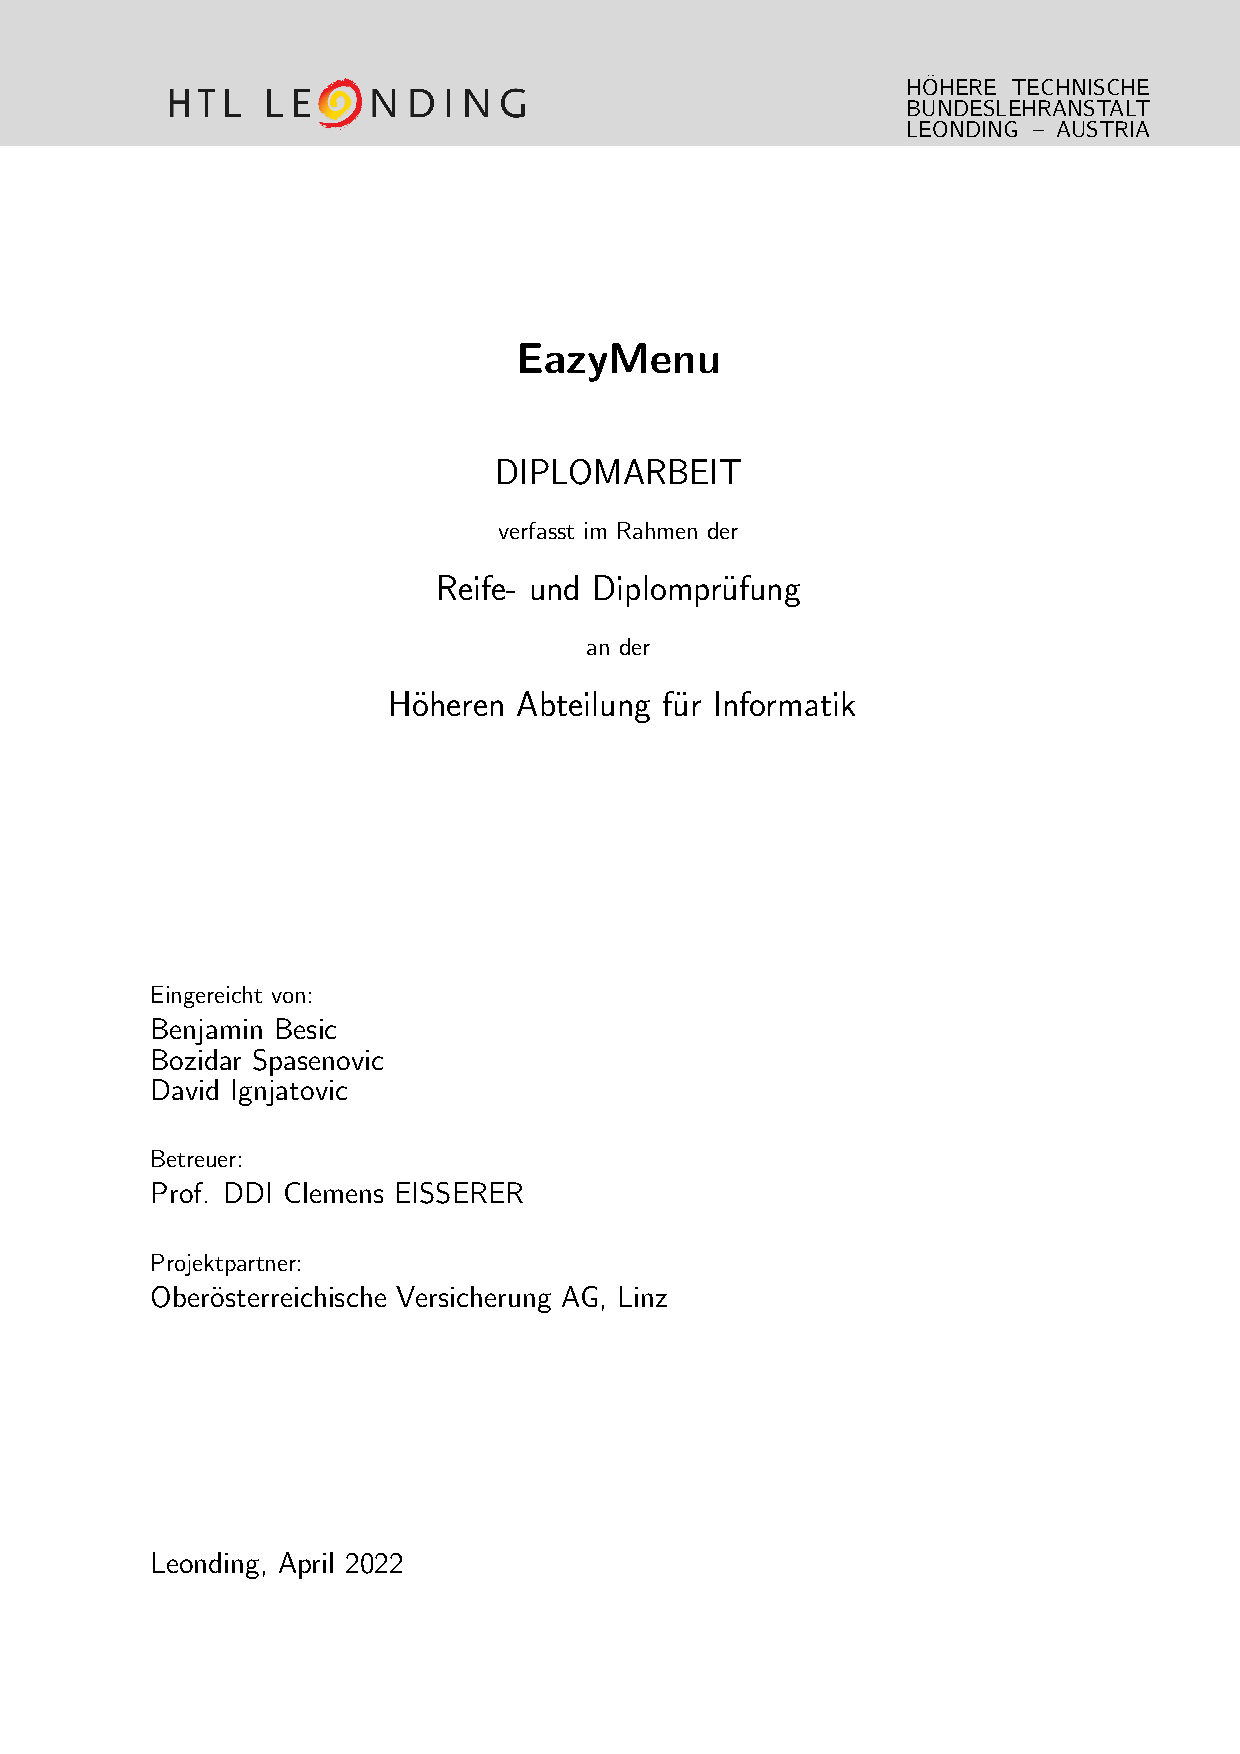
\includepdf{./titlepage/coversheet}
\pagenumbering{Roman}
\newpage
\thispagestyle{empty}
\vspace{3cm}
~ \\ \\
Ich erkläre an Eides statt, dass ich die vorliegende Diplomarbeit selbstständig und ohne fremde Hilfe verfasst, andere als die angegebenen Quellen und Hilfsmittel nicht benutzt bzw. die wörtlich oder sinngemäß entnommenen Stellen als solche kenntlich gemacht habe.

Die Arbeit wurde bisher in gleicher oder ähnlicher Weise keiner anderen Prüfungsbehörde vorgelegt und auch noch nicht veröffentlicht.

Die vorliegende Diplomarbeit ist mit dem elektronisch übermittelten Textdokument identisch.
\vspace{3cm}
% Hier kommt die Unterschrift drüber
\begin{tabbing}
Leonding, April 2022 \hspace{1cm} Benjamin Besic \& Bozidar Spasenovic \& David Ignjatovic
\end{tabbing}
\vspace{10cm}
Zur Verbesserung der Lesbarkeit wurde in diesem Dokument auf eine geschlechtsneutrale Ausdrucksweise verzichtet.
Alle verwendeten Formulierungen richten sich jedoch an alle Geschlechter.
\newpage
\setcounter{page}{1}

\begin{spacing}{1}
    \chapter*{Abstract}
\end{spacing}
\begin{wrapfigure}{r}{0.3\textwidth}
    \begin{center}
      
\includegraphics[width=0.4\textwidth]{pics/Logo-EazyMenue.png}
    \end{center}
\end{wrapfigure}
EazyMenu is an application for managing food orders in company canteens and was developed to replace an existing application used by Oberösterreichische Versicherung 
based on IBM Notes. 
This application was only accessible on the desktop and did not meet today's standards. 
EazyMenu instead allows employees to order a meal quickly and easily via their mobile phone or from a desktop. 
Meals can be categorized by tags. An algorithm then uses the tags to decide what meal should be suggested to an employee based on his previous orders. 
The cafeteria also has the ability to create new meals and manage them as well. 
It is also possible to print out an order overview with the most important information for a particular day.


\newpage

\begin{spacing}{1}
    \chapter*{Zusammenfassung}
\end{spacing}
\begin{wrapfigure}{r}{0.3\textwidth}
    \begin{center}
      
\includegraphics[width=0.4\textwidth]{pics/Logo-EazyMenue.png}
     \end{center}
\end{wrapfigure}
\author{David Ignjatovic}
EazyMenu ist eine Anwendung zur Verwaltung von Essensbestellungen in Firmenkantinen und wurde entwickelt, um eine Altapplikation der Oberösterreichische Versicherung auf Basis von IBM Notes abzulösen. 
Diese Altapplikation war nur auf dem Desktop zugänglich und entsprach nicht den heutigen Standards. 
Im Gegensatz dazu ermöglicht EazyMenu Mitarbeiterinnen und Mitarbeitern per Handy oder von einem Desktop aus schnell und einfach eine Mahlzeit zu bestellen. 
Dabei können Gerichte durch Tags kategorisiert werden. Ein Algorithmus entscheidet dann anhand der Tags, welche Mahlzeit einem Mitarbeiter auf Basis seiner bisherigen Bestellungen vorgeschlagen werden soll.
Auch die Kantine hat die Möglichkeit neue Mahlzeiten zu erstellen und diese auch zu verwalten. 
Es besteht auch die Möglichkeit eine Bestellübersicht mit den wichtigsten Informationen für einen bestimmten Tag auszudrucken.

\pagestyle{plain}

\renewcommand{\lstlistlistingname}{Quellcodeverzeichnis}

\tableofcontents
\newpage
\setcounter{RPages}{\value{page}}
\setcounter{page}{0}
\pagenumbering{arabic}
\pagestyle{scrheadings}

\begin{spacing}{1}
\chapter{Einleitung}\label{chapter:introduction}
\end{spacing}
\section{Ausgangsituation}
\author{Benjamin Besic}
Die Oberösterreichische Versicherung ist der Marktführer im Versicherungsbereich in Oberösterreich 
und beschäftigt in ihrer Zentrale in Linz über 500 Mitarbeiter.
Das Unternehmen besitzt eine Kantine, wo täglich 3 Hauptspeisen serviert werden. Zu jeder Hauptspeise gehört zusätzlich eine Vor- 
und Nachspeise.
\section{Ist-Zustand}
\author{Benjamin Besic}
Die derzeitige Bestellmöglichkeit funktioniert über eine simple Datenbankanwendung mit IBM Notes.
Dieses Programm ist auf jedem Rechner installiert und jeder Mitarbeitende ist mit seinen bzw. ihren Daten bereits eingeloggt.
Auf einem simplen Interface kann man zwischen den heutigen und zukünftigen Mahlzeiten wählen. Dazu kann man einen Zeitpunkt auswählen,
wann man eine Mahlzeit konsumieren will. 
Nach erfolgreicher Bestellung hat man eine kleine Übersicht über die vergangenen Bestellungen.
\section{Problemstellung}
\author{Benjamin Besic}
Das derzeitige Programm ist sehr veraltet und nicht besonders benutzerfreundlich. Außerdem
läuft das Programm lokal auf jedem Rechner und eine Bestellung unter Benutzung von mobilen Endgeräten ist nicht möglich.
Außerdem ist zu erwähnen ist, dass der Benutzer nur eine beschränkte Möglichkeit hat sein Bestellverhalten 
zu visualisieren bzw. zu analysieren.
\section{Aufgabenstellung}
\author{Benjamin Besic}
Die Aufgabenstellung war daher, eine Webanwendung zu entwickeln, die den Vorgänger ablöst
und ein modernes und benutzerfreundliches Interface hat. Zudem soll eine Bestellung über das Smartphone
möglich sein. Zusätzlich soll ein Empfehlungssytem entwickelt werden, dass einem ermöglicht Mahlzeiten zu 
bestellen, die auf einen abgestimmt sind. Außerdem soll es eine Einsicht über die Bestellhistorie geben
mit diversen Statistikelementen.
\section{Ziel(e)}
\author{Benjamin Besic}
\begin{itemize}
    \item Erleichterung des Bestellprozesses für den Benutzenden
    \item Flexible Bestellmöglichkeiten
    \item Der Benutzende hat bessere Einsicht über sein Bestellverhalten
\end{itemize}

\subsection{Zielgruppe}
Grundsätzlich ist das  Programm an die Mitarbeiter der OÖ Versicherung AG gerichtet. Doch das Projekt
könnte durchaus unter anderen Bedingungen für andere Firmen bzw. Einrichtungen umgesetzt werden.




\begin{spacing}{1}
\chapter{Planung}\label{chapter:planning}
\end{spacing}
\author{Benjamin Besic}
Der Anfang der Planung war die Besprechung des alten Programms und was an dem nicht passt bzw. verbessert gehört.

\section{Use Cases}

\subsection{Kantinenarbeiter}

\begin{compactitem}
    \item Neue Menüs anlegen
    \begin{compactitem}
        \item Ein Kantinenmitarbeiter kann für jeden Tag neue Menüs mit drei Hauptspeisen und deren Kategorien, einer Vorspeise und einer Nachspeise anlegen.
    \end{compactitem}
    \item Vorhandene Menüs editieren
    \begin{compactitem}
        \item Die Bezeichnungen der bereits erstellten Menüs sollen verändert werden können.
    \end{compactitem}
    \item Übersicht der täglichen Bestellungen
    \begin{compactitem}
        \item Die Kantinenmitarbeiter sollen eine Übersicht, der an einem bestimmten Tag bestellten Menüs haben. Diese inkludiert die zusammengefasste Bestellanzahl der verschiedenen Menüs und eine Liste von allen Bestellungen.
    \end{compactitem}
    \item Bestellungsübersicht drucken
    \begin{compactitem}
        \item Die Übersicht wie vorher beschrieben soll zu einem PDF-Objekt konvertiert werden und dementsprechend ausgedruckt werden können.
    \end{compactitem}
\end{compactitem}

\subsection{Mitarbeiter}

\begin{compactitem}
    \item Menüs bestellen
    \begin{compactitem}
        \item Ein Mitarbeiter hat eine Auswahl aller Menüs und kann für jeden Tag eine der drei Hauptspeisen auswählen. Nach der Auswahl kann er die Essenszeit auswählen, die Anzahl und nötige Kommentare hinzufügen.
    \end{compactitem}
    \item Menüs für andere Mitarbeiter bestellen
    \begin{compactitem}
        \item Ein Mitarbeiter kann den obrigen Bestellvorgang für einen anderen Mitarbeiter ausführen. 
    \end{compactitem}
    \item Übersicht aller Bestellungen
    \begin{compactitem}
        \item Als Mitarbeiter soll man alle seine vergangenen Bestellungen und deren Informationen in einer Übersicht einsehen können. Diese Übersicht kann filtriert werden.
    \end{compactitem}
    \item Bestellungen stornieren
    \begin{compactitem}
        \item In der oben genannten Übersicht soll man die Möglichkeit haben eine Bestellung auszuwählen und zu stornieren, wenn dies möglich ist.
    \end{compactitem}
    \item Bestellstatistiken einsehen
    \begin{compactitem}
        \item Ein Mitarbeiter soll Diagramme zur Verfügung haben, wo er sein Bestellverhalten einsehen kann.
    \end{compactitem}
\end{compactitem}
\pagebreak


\section{Datenmodell-Diagramme}
Der nächste Arbeitsschritt war die Entwicklung eines Datenmodells, welches die Basis der Programmlogik sein soll. Dieses wurde mit einem ERD-Diagramm erstellt.
\begin{figure}[htp]
    \centering
    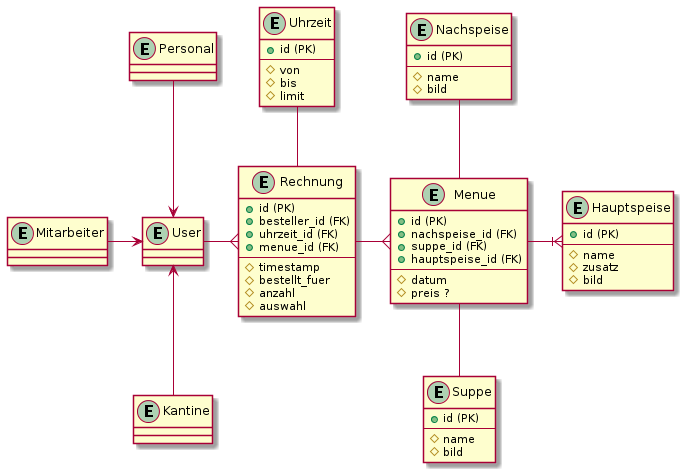
\includegraphics[scale=0.5]{pics/erd-alt.png}
    \caption{Erste Version des Datenmodells}
    \label{fig:impl:ERDold}
\end{figure}

\begin{figure}[htp]
    \centering
    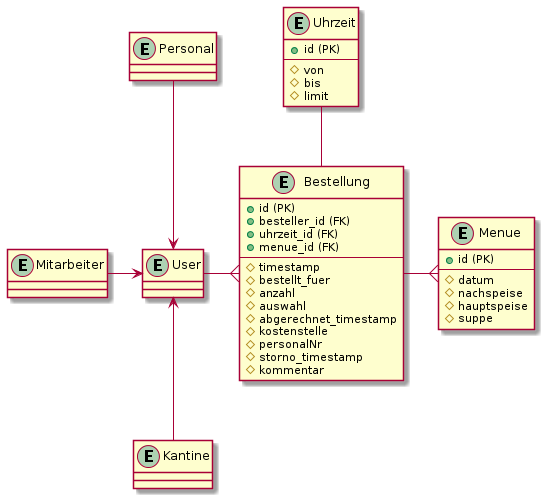
\includegraphics[scale=0.5]{pics/erd-aktuell.png}
    \caption{Finale Version des Datenmodells}
    \label{fig:impl:ERDnew}
\end{figure}
\pagebreak

\section{UI entwickeln}

Nachdem das Datenmodell feststand wurden UI-Prototypen entwickelt, die das Aussehen der Vue-App darstellen sollen.

\begin{figure}[htp]
    \author{Benjamin Besic}
    \centering
    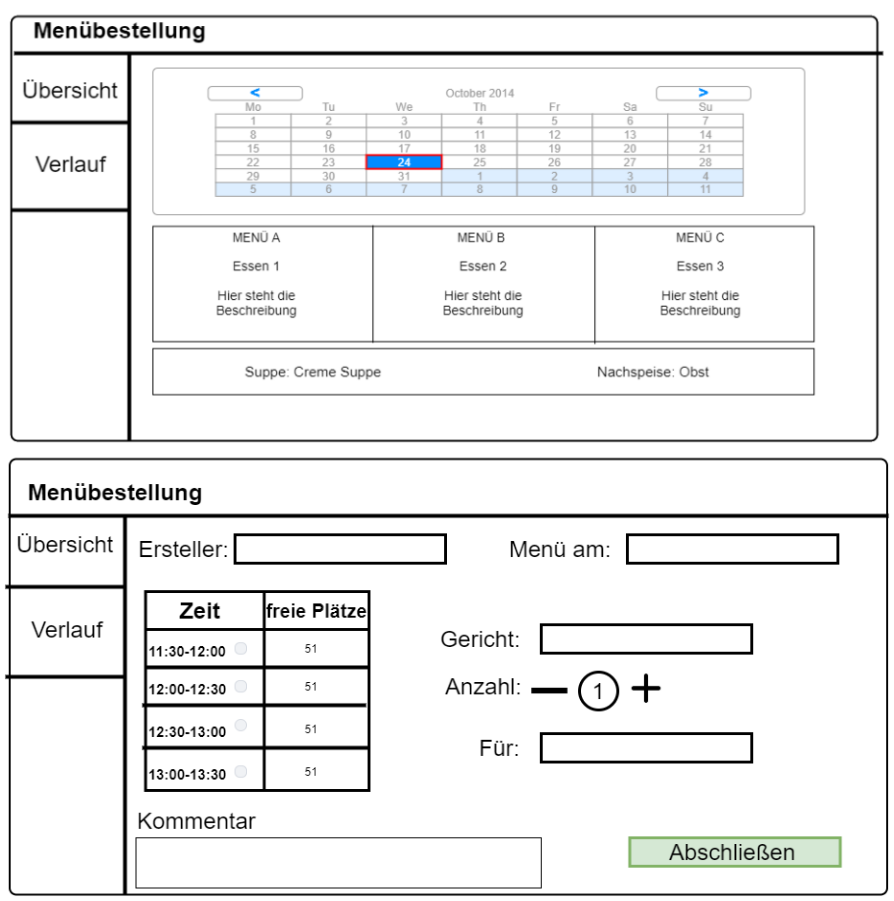
\includegraphics[scale=0.36]{pics/UI-Bestellung-Prototyp.png}
    \caption{UI-Prototypen für den Bestellvorgang}
    \label{fig:impl:UIPlanningBest}
\end{figure}

\begin{figure}[htp]
    \author{Benjamin Besic}
    \centering
    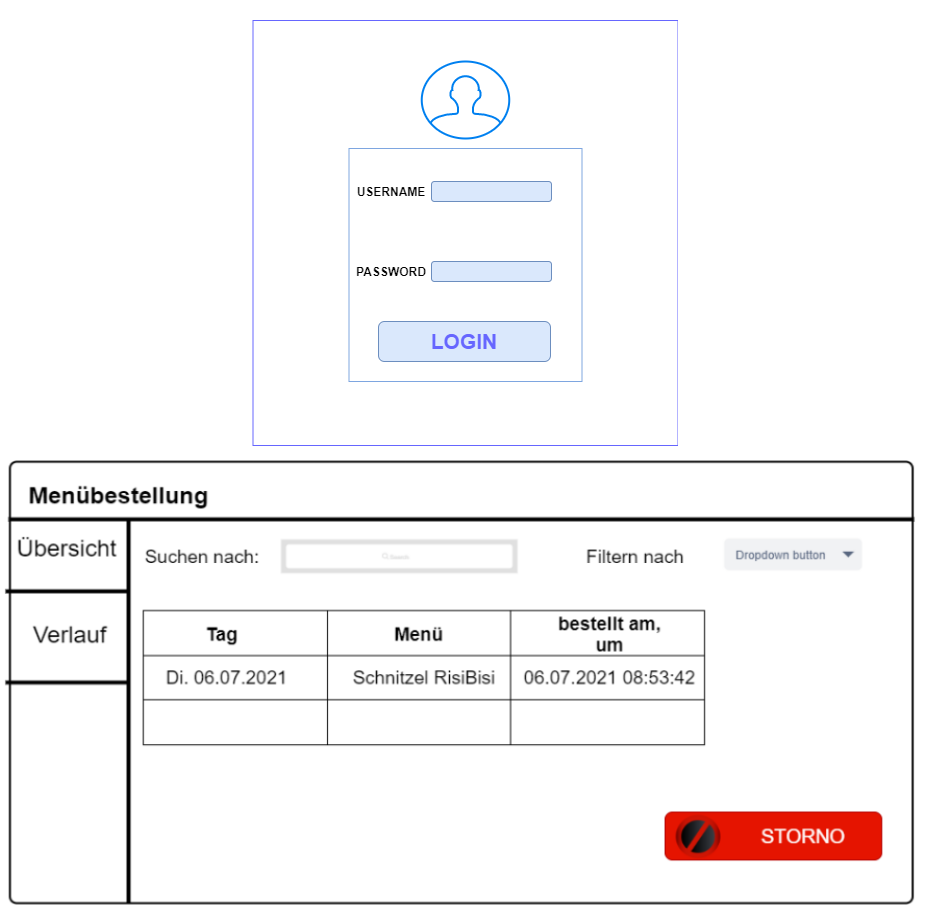
\includegraphics[scale=0.36]{pics/UI-Login-Uebersicht-Prototyp.png}
    \caption{UI-Prototypen für den den Login und die Übersicht}
    \label{fig:impl:UIPlanningLogUebersicht}
\end{figure}

\pagebreak

\section{Technologien}
Beim Entwickeln wurden folgende Technologien verwendet:
\begin{itemize}
    \item docker 3.1
    \item Vue.js 2.6.14
    \item quarkus 2.5.0.Final
    \item Jetpack Compose 1.0.1
    \item Keycloak 14.0.0
    \item Java OpenJDK-11
    \item Java EE 8
    \item JBoss Wildfly 7.3.4.GA
\end{itemize}

\begin{spacing}{1}
\chapter{State of Art}\label{chapter:state-of-art}
\end{spacing}
Die Oberösterreichische Versicherung hat das veraltete IBM-Notes Bestellsystem verwendet. Das hatte keine Möglichkeit Kategorien auszuwählen,
die Beestellübersicht mit Graphen und dem Vorschlagen des \textit{perfekten} Menüs für den Benutzer.

Die Webapp sollte nicht mit \textit{Lieferando},\textit{Mjam},\textit{Delivery Hero} oder \textit{Lieferheld} und weiteren verglichenn werden
da sie nur auf Gerichte der Kantine des Unternehemens spezifiziert ist.

\begin{spacing}{1}
\chapter{Verwendete Technologien}\label{chapter:tech}
\end{spacing}
\section{IntelliJ IDEA}
\author{Benjamin Besic}

IntelliJ IDEA ist eine der führenden Entwicklungsumgebungen für die Programmiersprache Java. Sie wurde vom Unternehmen Jetbrains im Jahre 2000 entwickelt.
\\* Außerdem bietet sie ebenfalls eine Programmierumgebung für Kotlin, Groovy, Scala und auch Android.
 Sie ist immer auf dem neusten Entwicklungsstand, wird laufend mit Updates versorgt und unterstützt die derzeit gängigen Programmiertools
wie Docker, Kubernetes, Maven, Datenbank-Tools, Git, Jakarta EE und viele weitere.
Es gibt eine kostenpflichtige Ultimate Version und eine Community Version, die kostenfrei zur Verfügung gestellt wird.
\\* IntelliJ zeichnet auch die Anzahl an Erweiterungen mittels Plugins aus. Die Umgebung besitzt auch eine
sehr intuitive Intelligenz, die es dem Entwickler sehr einfach macht damit zu programmieren. Diese Intelligenz beinhaltet z.B. Codevorschläge oder Vorschläge, um die Codequalität zu verbessern.
\cite{IntJ} \\*
Wir haben uns für die Verwendung entschieden, da wir damit viel Erfahrung hatten und die oben genannten Punkte
unterstützten unsere Entscheidung dabei.

\pagebreak
\section{Android Studio}
\cite{JetpackCompose-Overview}
\author{Bozidar Spasenovic}
Android Studio ist eine Entwicklungsumgebung für Android-Anwendungen. Es basiert auf IntelliJ.
\\* 
Neben dem leistungsstarken Code Editor werden noch mehr Funktionen bereitgestellt, um für die Produktivität zu verbessern. 
Android Studio funktioniert auf Windows, GNU/Linux, macOS und Chrome OS. Die erste Version kam nach zwei Jahren Entwicklungsdauer am 8. Dezember 2014 heraus.
Weiters beinhaltet es ein Gradle-build-system, viele verschiedene Androidemulatoren und ein Vorschaufenster mit der Anwendung.

\subsection{Apply Changes}
\cite{Android-Studio-ApplyChange}
Das ist eine sehr wichtiges Merkmal für alle Programmierer. Ab der Android Studio 3.5 Version ist es möglich, seinen Code
zur Laufzeit des Programmes zu ändern, ohne die Applikation zu schließen. Um dieses Merkmal benutzen zu können, muss man ein sogenanntes \textit{debug build variant} benutzen
und der Emulator muss die Version 8.0 oder höher haben.

Wenn man die Änderungen verwenden möchte hat man drei Möglichkeit:
\begin{itemize}
    \item Apply Changes and Restart Activity
    \item Apply Code Changes 
    \item Run 
\end{itemize}

Falls ein Problem auftaucht nachdem man \textit{Apply Changes and Restart Activity} oder \textit{Apply Code Changes} betätigt,
wird sofort vorgeschlagen die App mittels \textit{Run} zu starten. 

\subsection{Emulator}
Um eine App sehen zu können, benötigt man ein Emulator oder ein echtes Gerät. 
Der Android Emulator simuliert also nicht nur ein einzelnes Gerät sondern viele andere Versionen.
Somit kann man seine App auf mehreren Devices problemlos testen, auch wenn man nicht jedes besitzt.

Den Emulator kann genauso viel wie ein normales Handy. Anrufen, SMS, Standort sowie rotieren des Emulators ist kein Problem.
Einer der Vorteile zu einem echten Gerät ist die Schnelligkeit der Übertragungen von Daten. Android Studio bietet 
eine Vielzahl von Emulatoren für normale Handys, Tablets, Smart-Uhren und Android Fernseher. 



\section{Git}
\author{Benjamin Besic}
Git ist ein Versionskontrollsystem (oft abgekürzt durch VCS) für Entwickler. Es ist ein Open-Source System, das im Jahre 2005
von Linus Torvald entwickelt wurde. Laut einer Stack Overflow-Umfrage von Entwicklern nutzen über 87 \% der Entwickler Git.
\cite{GitKinsta}
\\* Zuallererst muss man den Begriff Versionskontrolle erklären, um Git zu verstehen.
\subsection{Versionskontrolle}
Diese dient dazu, um den originalen Quellcode effizient mit mehreren Personen editieren bzw. entwickeln zu können. 
\\* Die Entwickler arbeiten mit Verzweigungen und Zusammenführungen. Jeder Entwickler kann Änderungen sicher durchführen, ohne seine Kollegen dabei 
zu behindern. Diese Änderungen können dann, sobald sie funktionsfähig sind, wieder in den Hauptquellcode eingebunden werden.
Alle Änderungen sind nachvollziehbar und bei Bedarf kann man sie dann wieder zurücksetzen.
\cite{GitKinsta} \\*

\subsection{Git Funktionsweise}
Jeder Entwickler hat seine eigene Version des Projekts (Working Directory), die er frei bearbeiten kann. Diese bekommt man durch einen Klon des Projekts (\hyperref[sec:Clone]{Clone}). \\* Änderungen kann man aufteilen und 
in Paketen bereitstellen, nach dem man diese durch Commits trennt. Einen \hyperref[sec:Commit]{Commit} kann man benennen. \\*
Diese Commits kann man dann online veröffentlichen durch einen \hyperref[sec:Push]{Push}. Ein Push ist nur möglich, wenn man die aktuellste Version des Projekts
auf seinen Rechner gezogen hat (\hyperref[sec:Pull]{Pull}). 
Einem Push kann man einen bestimmten Zweig (\hyperref[sec:Branch]{Branch}) zuordnen. 
\begin{figure}[htp]
    \author{David Ignjatovic}
    \centering
    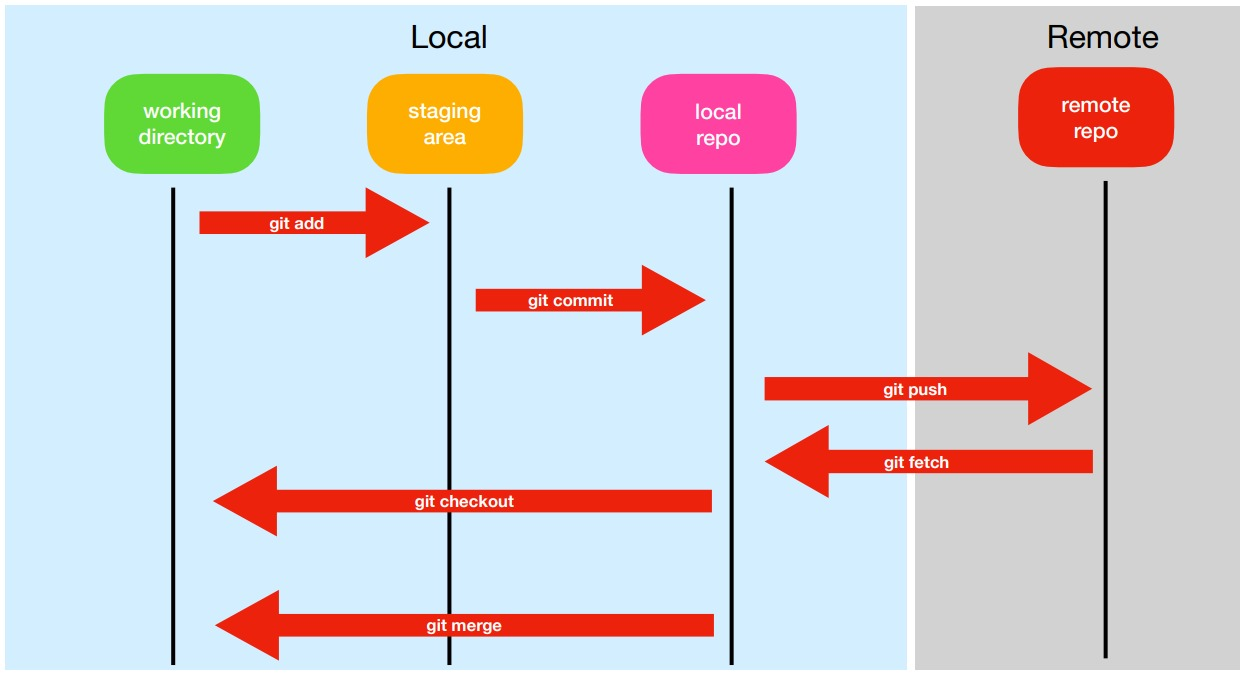
\includegraphics[scale=0.35]{pics/GitWorkflow.jpg}
    \caption{Darstellung des Git Workflows}
    \label{fig:impl:GitWorkflow}
\end{figure}
Diese Zweige dienen dazu, um das Projekt in verschiedene
unabhängige Teile zu trennen, falls man zum Beispiel an einer Demo Version weiterschreiben möchte. \\* Nach einem erfolgreichen Push sind die Änderungen
online auf dem Repository zu finden. Ein Repository ist der ``Ordner'', wo alle Dateien online gespeichert zu finden sind. 
\\* Ein Vorteil, den Git ebenfalls bietet ist, dass jeder Commit eine Version des Projekts ist, die man bis zum Zeitpunkt vom Commit herunterladen oder klonen kann.
Jedes Projekt kann privat oder öffentlich gemacht werden, sodass auch Personen, die keine Entwickler sind, darauf zugreifen können.
\cite{GitExpl} 



\subsection{Git Befehle}

\subsubsection{Clone}
\label{sec:Clone}
Es initialisiert ein Git Repository auf dem Rechner und ladet die zugehörigen Dateien runter.
Wenn man es nicht spezifisch angibt, klont es den Master Branch. Der Master Branch ist der Hauptzweig, eines jeden Git Projekts.
Innerhalb des erstellten Ordners können alle weiteren Git Befehle ausgeführt werden. \cite{GitCmnds}
\subsubsection{Commit}
\label{sec:Commit}
Ein Commit beschreibt Änderungen, die man im Projekt gemacht hat. Jeder Commit hat eine Bezeichnung, mit der der Entwickler die Änderungen,
die er gemacht hat beschreiben kann. Zu jedem Commit gehören auch die Dateien die dabei geändert bzw. hinzugefügt wurden.
\\* Der Commit speichert die Veränderungen, die seit dem letzten Commit gemacht wurden und dieser kann danach jederzeit abgerufen oder rückgängig gemacht werden.
Diese Änderungen bleiben aber zunächst nur lokal auf dem Rechner. \cite{GitCmnds}

\subsubsection{Push}
\label{sec:Push}

Ein Push dient dazu, um die lokalen Änderungen (Commits) zu veröffentlichen. Es kopiert den aktuellen, lokalen Stand und speichert diesen auf 
das vom Internet erreichbare Repository. \\* Einem Push kann ein Zweig (Branch) zugeordnet werden um die Änderungen zuzuordnen.
 \cite{GitCmnds}

\subsubsection{Pull}
\label{sec:Pull}
Der Pull Befehl kopiert die Inhalte vom öffentlichen Repository und fasst diese mit den lokalen Zustand auf dem 
Rechner zusammen (merge). Er dient dazu die aktuelle Version des Projekts auf den Rechner herunterzuladen.
\\* Falls es Konflikte zwischen der derzeitigen und neusten Version gibt, werden die Änderungen zusammengeführt. \cite{GitCmnds}

\subsubsection{Branch}
\label{sec:Branch}
Die Branch Befehle dienen dazu, um eine neue Abzweigung des Projekts (Branch) zu erstellen.
\\*
Branches erstellt man, wenn man an einer neuen Version des Projekts arbeitet und diese vom Hauptteil trennen will.
Meistens wird an neuen Funktionen gearbeitet, die später wieder in den Master Branch eingebunden werden.
\\* Der Vorteil daran ist, dass man an neuen Funktionalitäten experimentieren kann, ohne den Hauptentwicklungsstand zu 
beeinflussen. Branches können jederzeit gelöscht oder wieder ins Hauptprojekt integriert werden.
Es kann simultan am Master Branch und an Nebenzweigen gearbeitet werden durch trennen mit dem Push Befehl. \cite{GitExpl}

\begin{figure}[htp]
    \author{David Ignjatovic}
    \centering
    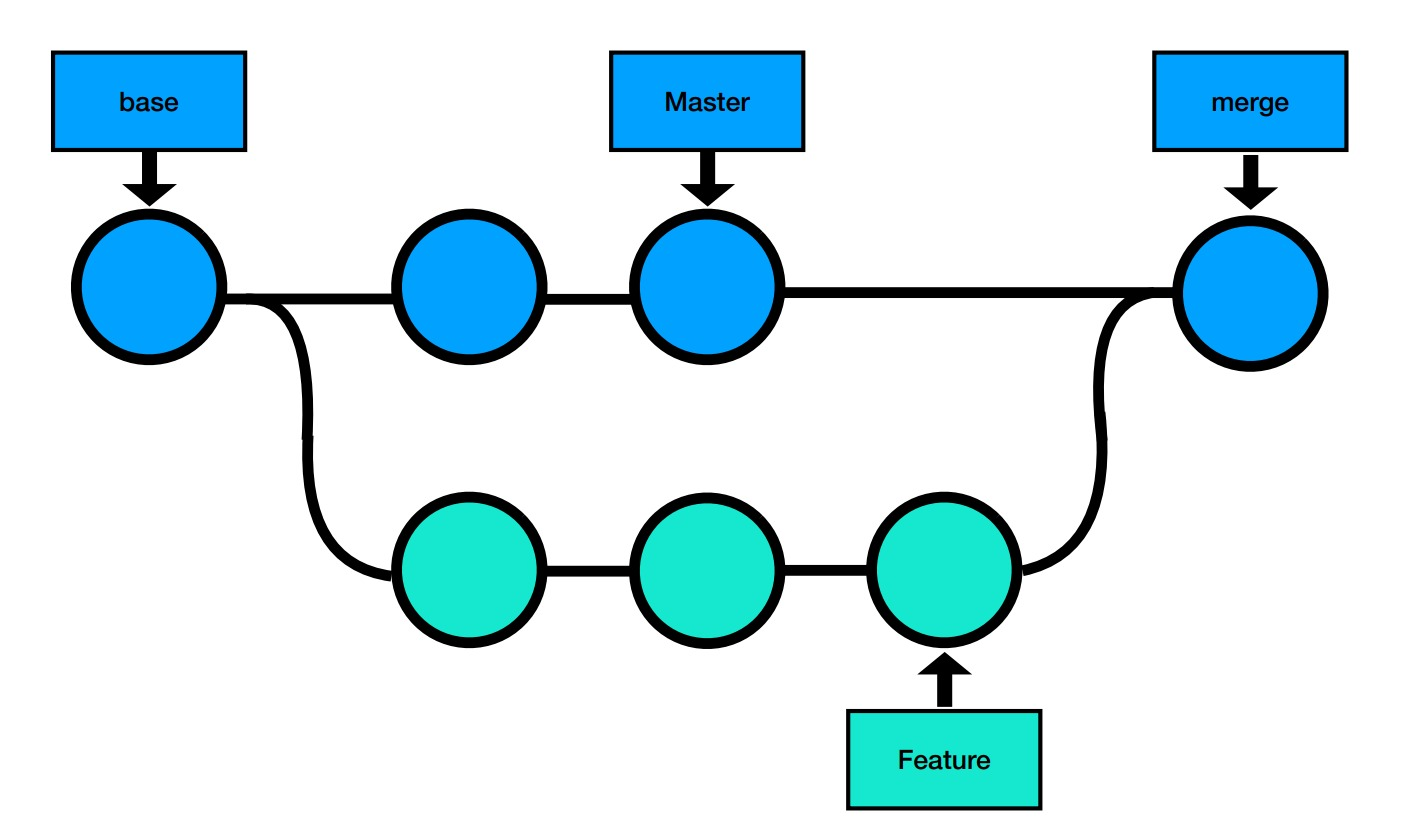
\includegraphics[scale=0.3]{pics/GitBranches.jpg}
    \caption{Darstellung von Branches in einem Repository}
    \label{fig:impl:GitBranches}
\end{figure}

\subsection{GitHub}
GitHub ist ein gewinnorientiertes Unternehmen, das einen auf Cloud basierten Git Repository Hosting-Service anbietet.
Es wurde im Februar 2008 gestartet und von Chris Wanstrath, PJ Hyett, Scott Chacon und Tom Preston-Werner entwickelt.
Es ist das beliebteste Tool um Softwareprojekte zu verwalten und wird von über 73 Millionen Entwicklern und über 4 Millionen Organisationen
benutzt. Es ist das größte und am meisten fortgeschrittene Entwicklungssystem, das es gibt. \cite{GitHub} \\*
Es vereinfacht die Nutzung von Git für Teams und auch Einzelpersonen. 
Jeder kann sich einen GitHub Account erstellen und direkt loslegen und seine Arbeiten auf Repositories veröffentlichen.
Es ist nicht nur für Code-basierte Projekte verwendbar sondern auch Websiten erstellen und das Schreiben von Büchern ist möglich.
\\*
Was GitHub ausmacht ist die Benutzerfreundlichkeit und die Integration von Git. Außerdem bietet Github viele andere Funktionen wie zum Beispiel ein Projekt Board an,
was es erleichtert innerhalb eines Teams, Probleme besser lösen zu können. In diesem Board können alle Probleme aufgelistet werden und dementsprechend können Teammitglieder zu bestimmten Problemen 
zugeteilt werden.   \\*
Es gibt ebenfalls Finanzierungspläne, die es vor allem Organisationen und Unternehmen leichter machen Unternehmensprojekte zu verwalten durch zusätzliche Funktionen. \cite{GitKinsta}
Diese Funktionen wären zum Beispiel:
\begin{itemize}
    \item Mehr Speicherplatz für das Repository
    \item Branches können bestimmten Nutzern zugeteilt werden 
    \item Es kann eine Prüfung durch Dritte bei Branchänderungen erforderlich gemacht werden
    \item Bessere Möglichkeit nachzuvollziehen, wer, was, wann gemacht hat durch detaillierte Logs
    \item Und viele weitere ...
\end{itemize}



\section{GitHub Actions}
\label{sec:GHAction}
\author{Benjamin Besic}

GitHub Actions ist eine von GitHub entwickelte Plattform, die das Automatisieren von verschiedenen Aspekten eines Softwareprojekts in Form von Pipelines ermöglicht.
Dabei handelt es sich um das Kompilieren, Testen und das Deployment eines Projekts. \\*
Es implementiert die beiden Methoden \hyperref[sec:CI]{CI} und \hyperref[sec:CD]{CD}. \cite{GHAction}

\subsection{CI und CD}
CI und CD sind zwei zusammenhängende Methoden, um Entwicklern das Programmieren an einem Projekt zu vereinfachen. Ebenfalls wird die Bereitstellung 
an den Kunden vereinfacht. \\*

\begin{figure}[htp]
    \centering
    \author{RedHat}
    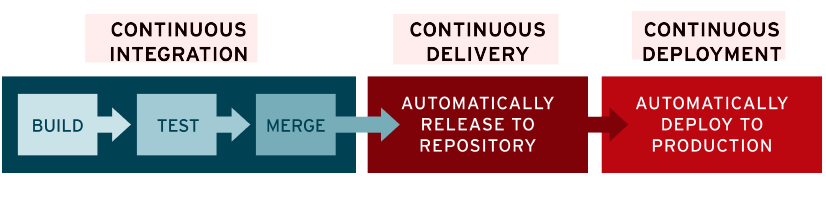
\includegraphics[scale=0.5]{pics/ci_cdi_grafik.png}
    \caption{Zusammenhang zwischen CI und CD}
    \small \url{https://www.redhat.com/cms/managed-files/ci-cd-flow-desktop_edited_0.png} 
    \label{fig:impl:CICD}
\end{figure}

\subsubsection{CI (Continuous Integration)}
\label{sec:CI}
CI steht für "Continuous Integration", dies beschreibt den Prozess der Automatisierung aus der Sicht eines Programmierers. \\*
Wenn mehrere Entwickler gleichzeitig an einem neuen Feature arbeiten, kann es passieren, dass der Code beim Zusammenführen oft die Funktionsfähigkeit des Programms beeinträchtigt.
CI soll dies verhindern, indem es einen automatisierten Prozess bereitstellt, der die Funktionsfähigkeit eines Programms validiert mittels Tests, nach jeder Zusammenführung.\\* Dies erlaubt 
es den Entwicklern, den Code öfter zusammenzuführen, sogar eine tägliche Zusammenführung ist dadurch manchmal möglich \cite{RHatCICD}

\subsubsection{CD (Continuous Delivery/Deployment)}
\label{sec:CD}
CD steht für ``Continuous Delivery'' bzw. ``Continuous Deployment'', dies sind zwei Konzepte die immer gemeinsam genutzt werden. \\*
Continuous Delivery sorgt dafür, dass Änderungen eines Entwicklers automatisch in ein Repository veröffentlicht werden. Danach können diese Änderungen sofort in einer Produktionsumgebung
dargestellt werden. \\*
Nach der Delivery kommt das Continuous Deployment, dies stellt dem Kunden finale Änderungen am Programm, durch einen automatisierten Prozess zur Verfügung.
Das heißt, nachdem die Entwickler zufrieden sind mit einer Version, können sie diese veröffentlichen und der Kunde kann das Programm dann benutzen.\cite{RHatCICD}
\pagebreak

\begin{figure}[htp]
    \centering
    \author{Percy Bolmer}
    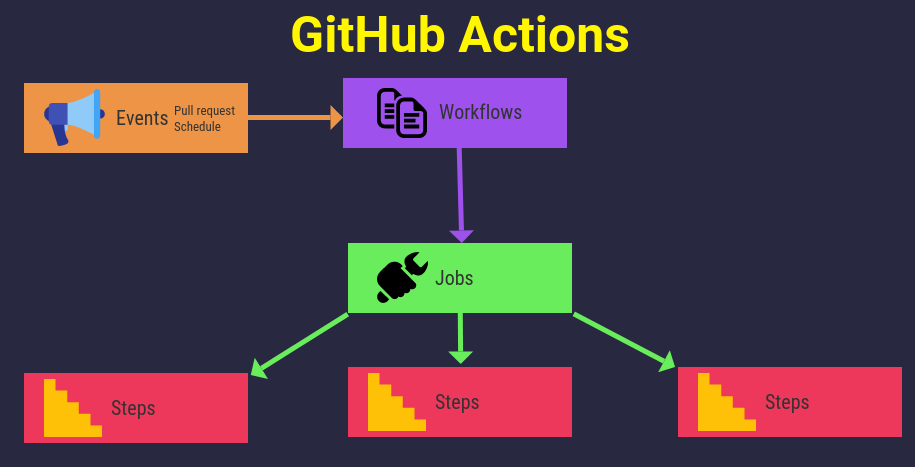
\includegraphics[scale=0.4]{pics/gh_actions_grafik.png}
    \caption{Ablauf von Github Actions}
    \small \url{https://miro.medium.com/max/1400/1*8Agtv-SaM-zw_GLzPI7p5w.png} 
    \label{fig:impl:GHActionAb}
\end{figure}

\subsection{Workflows}
GitHub Actions benutzt Workflows, um Arbeitsschritte, die zusammenhängen, gemeinsam auszuführen. Zum Beispiel gibt es Workflows zum Deployen, nur zum Testen oder um eine Dokumentation hochzuladen.\\*
Ein Workflow ist ein automatisierter Prozess, der einen oder mehrere Jobs ausführt.
Diese werden mittels eines .yaml-File beschrieben. Ein Workflow wird durch ein bestimmtes Event ausgeführt, z.B. ein Push auf den main-Branch. Mann kann es aber auch manuell oder nach einem
bestimmten Zeitplan ausführen. \cite{GHAction}

\begin{lstlisting}[language=yaml,caption=Ausschnitt eines Workflow Files]
# Workflow Bezeichnung
name: Publish EazyMenue Frontend and Backend

# Definiert wann der Workflow ausgefuehrt wird 
on:
  # Trigger wenn ein Push auf den main Branch erfolgt
  push:
    branches: ['main']

# Jobs die nacheinander oder parallel ausgefuehrt werden
jobs:
  build_backend:
    name: Build backend
\end{lstlisting}

\subsection{Event}
Ein Event ist eine Aktivität, die einen Workflow ausführt. Er dient als sogenannter Trigger.
Ein Event könnte z.B. ein Push auf einen Branch sein oder ein Pull Request etc.\cite{GHAction}

\subsection{Jobs}
Ein Job hat mehrere Steps (Stufen), die nacheinander ausgeführt werden. Ein Step kann z.B. ein Shellscript File sein, ein
Login in ein anderes Repository oder eine vordefinierte Action. Der Jobs fasst diese Steps zusammen und die Steps können untereinander die selben Ressourcen nutzen.\cite{GHAction}

\begin{lstlisting}[language=yaml,caption=Ausschnitt eines Jobs]
    build_backend:
    name: Build backend
    # Der Job wird in einem Ubuntu Container ausgefuehrt
    runs-on: ubuntu-latest
    env:
    # Unter env kann man sich Variablen definieren
      IMAGE_NAME: eazy-menue-backend
    defaults:
      run:
      # Es wird der backend-Ordner aus dem Repo genommen
        working-directory: ./eazy-menue-backend
    steps:
      - name: Check out the repo
        uses: actions/checkout@v2
      - name: Package
        run: mvn package -DskipTests
      - name: Build image
        run: docker build . -f src/main/docker/Dockerfile.jvm --tag $IMAGE_NAME
\end{lstlisting}

\subsection{Actions}
Die GitHub Actions Plattform stellt verschiedene vordefinierte Actions zur Verfügung.
Eine Action führt eine bestimmte komplexe Aufgabe aus, die auch oft benutzt wird in Workflows. Diese Actions helfen dabei,
um die Redundanz von bestimmtem Code bzw. Codeblöcken zu vermeiden.
Actions umfassen z.B.: ein Repository pullen oder sich bei einem Dienst zu authentifizieren.\\*
Es ist auch möglich selber Actions zu schreiben, falls man keine passende auf dem GitHub Marketplace findet.\cite{GHAction}

\section{Github Packages}
\author{Benjamin Besic}
GitHub Packages, entwickelt von GitHub, ist ein Dienst, der es ermöglicht Software-Pakete hochzuladen und diese privat oder öffentlich zu nutzen.
Dies beinhaltet Softwarecontainer und Dependencies. \\*
Das Ziel von GitHub Packages ist es den Code und die Software selbst auf einer Plattform zusammen zu Verfügung stellen zu können.
Der ganze Entwicklungsprozess ist somit auf GitHub zentralisiert. Zusammen mit \hyperref[sec:GHAction]{GitHub Actions} kann man die Veröffentlichung
komplett automatisieren. \\*
Es stellt Package Registries (Sammlungen) für die gängigsten Package Manager wie npm, RubyGems, Apache Maven, Docker (Docker Images), 
NuGet und Gradle zur Verfügung. \cite{GHPack}

Nützliche Funktionen von GitHub Packages sind:
\begin{itemize}
    \item Rechte: Man kann bestimmen, wer die Packages ändern bzw. wer diese sehen und benutzen darf.
    \item Sichtbarkeit: Man kann einstellen ob das Package nur privat oder öffentlich nutzbar ist.
\end{itemize}

\subsection{Github Container Registry (ghcr.io)}
Die GitHub Container Registry (ghcr) ist aus den Packages entstanden, um eine eigene Plattform für Softwarecontainer zu haben, die zu GitHub gehört.
Somit wird GitHub noch mehr in die Entwicklung integriert. \\*
Man kann es mit DockerHub vergleichen, eine Plattform um Docker Images hochzuladen und an einem Ort zu sammeln. 
Es besteht ebenfalls die Möglichkeit, Docker Images auf das ghcr hochzuladen, anstatt DockerHub zu benutzen. \\*
Es hat dieselben Rechte- und Sichtbarkeitsfunktionen wie oben genannt. Darüber hinaus kann man auch verschiedene Versionen eines Images und Statistiken
über die Nutzung einsehen.\cite{GHContReg} 


\section{Java}
\author{David Ignjatovic} 

Die relativ junge Programmiersprache Java, welche 1995 entwickelt wurde, weckte schon von Beginn an das Interesse der Programmiergemeinschaft. \cite{Java} \\*
Die Programmiersprache Java ist Teil der Java-Technologie. 
Sie besteht aus dem sogennaten Java Development Kit (JDK). Die JDK wird dann verwendet um Java-Programme zu erstellen und die Java Runtime Environment (JRE) um diese
auszuführen.    
Die Programmiersprache selbst sollte aber nicht gleichgesetzt werden mit der Java-Technologie. \cite{JavaSprache}

\subsection{Hello World}
\author{David Ignjatovic} 
\begin{lstlisting}[language=Java,caption=Java File HelloWorld,label=lst:impl:foo]
public class HelloWorld {
    public static void main (String[] args){
            // Ausgabe Hello World!
            System.out.println("Hello World!");
    }
}
\end{lstlisting}

\subsection{Java Runtime Environment }
\author{David Ignjatovic} 

Java Runtime Environment (JRE) führt Software aus, die in der objektorientierten Programmiersprache Java geschrieben ist. 
Denn bei Java benötigt der Computer im Vergleich zur Programmiersprache C eine Laufzeitumgebung „Java Runtime Environment“ für das Betriebssystem, um Java-Programme ausführen zu können. \cite{JRE}

\subsection{Java Virtual Machine}
\author{David Ignjatovic} 

Java Virtual Machine (JVM) ist eine virtuelle Maschine, welche plattformunabhängige Anwendungen ermöglicht.
Die Plattformunabhängigkeit wird in Java durch das Zusammenspiel zweier Programme gelöst: \\*
Der Compiler wandelt den Quelltext, also die .java-Dateien, in einen sogenannten Java-Bytecode um. Der Interpreter (Virtual Machine) führt dann den Java-Bytecode aus. \cite{JVM}

\subsection{Java Byte-Code}
\author{David Ignjatovic} 

Bytecode in Java ist der Grund dafür, dass Java plattformunabhängig ist. Sobald ein Java-Programm kompiliert wird, wird der Bytecode generiert. 
Genauer gesagt ist ein Java-Bytecode ein Maschinencode in Form einer .class-Datei.

\section{JUnit}
\author{David Ignjatovic} 

JUnit ist ein Test Framework welches von Erich Gamma und Kent Beck entwickelt wurde. \cite{JUnit}
Damit man ganz einfach einen beliebigen Java Code überprüfen und zu testen kann, verwenden wir JUnit. \\*

Um JUnit zu verwenden, brauchen wir, wie schon erwähnt, einen beliebigen Java Code, welchen der Programmierer geschrieben hat. 
Mithilfe von sogenannten Unit Tests werden dann einzelne Testfälle von verschiedenen Klassen getestet.\\*

Beispiel für einen Unit Test (assertEquals): 

\begin{lstlisting}[language=Java,caption=Java File JUnit 1,label=lst:impl:foo]
    @Test
    public void t02_MenueTest_CreateMenueShouldBeSchnitzel(){
        Menue menue = new Menue();
        menue.setMainDish("Schnitzel");

        assertEquals(menue.getMainDish(),"Schnitzel");
    }
\end{lstlisting}

Beispiel für einen Unit Test (assertNotEquals): 

\begin{lstlisting}[language=Java,caption=Java File JUnit 2,label=lst:impl:foo]
    @Test
    public void t03_MenueTest_CreateMenueShouldNotBeSuppe(){
        Menue menue = new Menue();
        menue.setMainDish("Schnitzel");

        assertNotEquals(menue.getMainDish(),"Suppe");
    }
\end{lstlisting}


Die Akuelle JUnit Version, welche wir verwenden, heißt JUnit 5. Diese Version setzt sich aus mehreren Modulen zusammen. JUnit 5 besteht aus JUnit Platform + JUnit Jupiter + JUnit Vintage.

\section{Karate}
\author{David Ignjatovic} 

Karate wird verwendet, um Enpoints testen zu können. Die Syntax ist sehr einfach und leserlich für Menschen, die wenig bis keine Programmierkenntnisse haben.
Karate selbst testet nicht nur Enpoints, sondern erstellt auch HTML Reports, welche alle Testfälle dokumentiert und anzeigt. \\*

Einzelne Testfälle bezeichnet man in Karate als Scenarios. In diesen Scenarios werden dann CRUD Operationen getestet. Den Path der Abfrage und die einzelnen 
Parameter werden in den Scenarios mitgegeben, aber auch was für ein Response code zurückkommen soll.



\section{Java EE}
\author{David Ignjatovic} 

Die Enterprise Edition der Java Plattform (JEE), ist eine Spezifikation der Java-Plattform. 
Der wichtigste Bestandteil von Java EE sind die Webanwendungen. Um solch eine Anwendung ausführen zu können, wird eine Applikationsserver verwendet, welcher 
in mehrere Systeme unterteilt wird, die auch Container genannt werden. Für eine Webanwendung reicht meistens ein einzelner Web-Container aus. \\*

Die erste Version von Java EE, welche damals noch Java2EE genannt wurde, erschien 1990. Im Jahr 2003 wurde der Name der Plattform auf Java EE geändert.
Die erste völlig ausgebaute Version von Java EE, welche wir bis heute noch kennen, erschien im Mai 2006 und trug die Versionsnummer 5. 
2009 folgte die Version 6 und 2013 die Version 7.

Wie schon bereits erwähnt, wird zum Ausführen einer Java EE Webanwendung ein Applikationsserver verwendet. 
Die am häufigsten verwendeten Applikations-Server sind unter einer freien Lizenz verfügbar (sogenannte Open-Source-Software).
Beispiele für solche Servere währen Apache Geronimo und GlassFish. 
Als Alternative zu einem vollständigen Applikationsserver können auch Programme verwendet werden, welche nur einen Web-Container implementieren.
Diese Web-Container werden oft auch als Servlet- oder JSP-Container bezeichnet und sind meistens dafür ausrecheichend. Der bekannteste Web-Container ist Apache Tomcat.

\cite{JavaEE}

\section{Quarkus}
\author{David Ignjatovic} 

Quarkus ist ein Cloud-nativer Stack welcher von Red Hat entwickelt wurde. Es basiert auf den Jakarta EE- und Micro Profile-Standards. 
Eine Quarkus-Applikation hat gegenüber einem Konkurrenzprodukt eine deutlich kürzere Startzeit und einen erheblich geringeren Speicherbedarf, was ein großer Vorteil ist für das Serverless Computing.  \cite{Quarkus} \\*

Mit Quarkus hat man die Möglichkeit, Applikationen für die moderne, Cloud-native Welt zu erstellen. 
Es ist ein Kubernetes-natives Java-Framework, welches auf GraalVM und HotSpot angepasst wurde. \\*   

Im März 2019 wurde Quarkus, nach mehr als einem Jahr interner Entwicklung, der Open-Source-Community vorgestellt

\subsection{Java EE vs. Quarkus}
\author{David Ignjatovic} 

Der größte Unterschied zwischen Java EE und Quarkus ist, dass man bei Quarkus keinen Application Server benötigt. 
Ein weiter Vorteil wäre, dass bei Quarkus keine war-File erstellt wird, sondern eine jar-File, welche sehr klein ist. 
In diesem jar-File befinden sich auch noch die einzelnen Libaries, welche für die Webanwendung verwendet werden. \\*

Bei Java EE wird eine war-File erstellt. Noch dazu befinden sich auf dem JEE-Application Server schon viele Libraries die schon vorinstalliert sind. 
Der größte Nachteil von Java EE ist, dass man auch für kleine Anwendung einen ganzen Application Server braucht. \\*

Im Großen und Ganzen kann man sagen, dass Quarkus hier besser ist, da es sehr praktisch und schnell ist. 
Noch dazu ist Quarkus relativ neu und kann sich im Laufe der Jahre noch umso mehr verbessern. \\*

Am Anfang g haben wir Java EE gewählt, da es vom Auftraggeber vorgesehen war. Mit Java EE haten wir einige Probleme wie zum Beispiel die Zeit zum deployen. 
Mit Quarkus aber haben wir uns sehr viel Zeit gespart und konnten dadurch auch mehr Zeit in andere Sachen investieren wie zum Beispiel in das Testen.

Die Konfiguration bei Quarkus war auch um einiges einfacher als bei Java EE. Bei Quarkus findet die Konfiguration in den sogenannten \textbf{Application.Properties} statt.
Bei Java EE war die Konfiguration auf dem Application Server. Hier gab es nicht nur eine File zum konfigurieren sondern mehrere .xml Files. 
Das war ebenso noch ein Grund weshalb wir uns zum Schluss doch noch für Quarkus entschieden haben.


\subsection{JPA}
\author{David Ignjatovic} 

Java Persistence API (JPA) ist eine API welche für Datenbankzugriffe und für das objektrelationale Mapping verwendet wird. 
Objektrelationales Mapping (ORM) zeigt eine objektorientierte Sicht auf Tabellen und Beziehungen in relationalen Datenbank-Management-Systemen an.  \\*

Enterprise Applikationen führern üblicherweise viele Operationen auf Datenbanken durch.
Durch die Hilfe von JPA (Java Persistance API) wird der Aufwand reduziert, welcher benötigt wird, um mit der Datenbank zu kommunizieren. \\* \cite{JPA}

JPA wurde von JSR 220 Expert Group entwickelt und im Mai 2006 erstmals veröffentlicht.


\subsection{Hibernate}
\author{David Ignjatovic}

Hibernate wird oft als Object Relational Mapping Tool bezeichnet. Es ist ein Framework zur Abbildung von Objekten in einer relationaler Datenbank für die Programmiersprache Java.
Hibernate implementiert die Java Persistence API (JPA) und bietet Funktionalitäten wie zum Beispiel abfragen auf einer Datenbank mit der sogenannten Hibernate Query Language (HQL). \\*

Es wurde von JBoss im Jahr 2001 entwickelt und veröffentlicht. Somit ist auch Hibernate in dem JBoss Applikations-Server integriert .\cite{Hibernate}

\section{JBoss}
\author{David Ignjatovic}

JBoss ist ein Tochterunternehmen von Red Hat, welches Unterstützung für die gleichnamige Server-Plattform (JBoss Application Server) 
und zugehörige Services unter der Marke JBoss Enterprise Middleware Suite (JEMS) bietet. \cite{JBoss}

\subsection{JBoss Application Server}

Der JBoss Application Server ist eine J2EE-Plattform. Mithilfe von J2EE werden standardisierte, modulare Komponenten verwendet.
JBoss ist ebenfalls innerhalb des Amazon Cloud-Services EC2 verfügbar. \cite{JBoss}

\subsection{Panache}
\author{David Ignjatovic}

Panache ist eine Quarkus-spezifische Bibliothek, welche die Entwicklung einer Hibernate-basierten Persistenzschicht vereinfacht. 
Panache ersetzt den größten Teil des Boilerplate-Codes mit einfachen Methoden die man in die Quarkus Anwendung implementieren kann. 
Methoden wie create, update, and remove aber auch eigene Abfragen auf der Datenbank werden von Panache zur Verfügung gestellt. \\* \cite{Panache}


\section{Maven}
\author{David Ignjatovic}

Apache Maven ist ein leistungsfähiges Werkzeug, welches immer wieder vorkommende Prozeduren automatisiert und vereinfacht. 
Es wird oft als \textbf{Build Management System} bezeichnet und ist Teil vom \textbf{Software Configuration Management (SCM)}.  \\* \cite{Maven}

Neben Maven gibt es auch noch ANT, welches eher kommandoorientiert arbeitet. Maven ist eher strategisch orientiert, realisiert mehr Abstraktionen, wird deklarativer gesteuert, 
berücksichtigt Abhängigkeiten besser und ist besonders für aufwändigere Multimodulprojekte geeignet. \cite{Maven}

\section{Cypress}
\author{Bozidar Spasenovic}
\cite{Cypress-Docu}
Cypress ist eine JavaScript Framework, welches 2020 auf den Markt kam. Der CEO von Cypress ist Drew Lanham.
Da es kostenlos für jeden ist, hat Cypress somit eine gute Position unter den Entwicklern eingenommen.
Mit Cypress ist es hat man die Möglichkeiten seine Webapplikation zu bestimmten Anwendungsfällen zu testen.
Ein Anwendungsfall wäre eine Bestellung aufzugeben, eine vorhandene Bestellung löschen oder einzelne Menüs zu erstellen und kategorisieren.


Mit Cypress ist es möglich solche Beispiele aufzuzeichnen und es mehrere Male abspielen zu lassen. Somit wird der Input vom User 
von Cypress übernommen. 

Die Vorteile davon sind:
\begin{itemize}
    \item schnelles Testen
    \item Inputfehler vermeiden
    \item leicht konfigurierbar
    \item Fehleranalyse leichter
\end{itemize}

Cypress bietet aber noch mehr Funktionen an. Man kann sehen was der nöchste Schritt ist, somit kann man es auch Debuggen.
Es ist aber auch oft von Vorteil wenn man eine Bildschirmaufnahme oder Fotos hat. Somit ist man ständig in der Lage einen 
Fehler nachzuvollziehen.

Es gibt drei Arten von Tests:

\begin{itemize}
    \item End-To-End
    \item Integration
    \item Unit
\end{itemize}



\pagebreak
\section{Keycloak}
\author{Benjamin Besic}
Keycloak ist eine Open-Source Software, die Single-Sign-On mit Identity und Access Management für moderne Applikationen bereitstellt. Der erste Release war 2014 als Wildfly Community Projekt, seit 2018 aber steht es unter der Verwaltung von RedHat. \cite{KeycloakWiki}  \\* 
Es hat mehrere Distributionen und ist mit einer Vielzahl von Frameworks und Tools kompatibel bzw. bietet es eine Unterstützung dafür an. Zu diesen Frameworks zählen z.B.: Quarkus, Angular, Vue.js, Spring, usw. \cite{KeyCloakDZone}

\subsection{Distributionen}
\subsubsection{Server}
Die Standalone-Applikation ist downloadbar als .zip auf der Keycloak Seite. Es gibt zwei Versionen vom Server, zu einem die Wildy Application Server Version und auch eine Version, die über Quarkus läuft.
\subsubsection{Docker Image}
Genau so wie beim Server gibt es auch hier zwei verschiedene, offizielle Docker-Images, eines, das auf dem Wildfly Server basiert und eines, das auf Quarkus basiert.
\subsubsection{Operator}
Dies ist eine Distribution für Kubernetes und OpenShift, basierend auf der Operator SDK. \cite{KeyCloakDZone}
\subsection{IAM (Identity Access Management)}
\label{sec:IAM}
Eine der Hauptfunktionen von Keycloak ist das IAM. \\*
IAM oder auch IdM (Identity Management) ist ein Framework, das zum Authentifizieren von Benutzern und deren Rechten genutzt wird. \\*
Es prüft ob der Benutzer Zugang zu bestimmten Bereichen, Dateien und anderen Ressourcen hat, auf die er zugreifen will. Es prüft auch, wer diese Rechte verändern darf.
IAM-Systeme stellen auch nützliche Admin-Tools zur Verfügung, um z.B. Nutzerrechte zu ändern oder die Aktivität von Benutzern zu verfolgen. \cite{KeycloakMakeIT} \\*
IAM hat vier Hauptfunktionen:
\begin{itemize}
    \item \textbf{Die Identitäts-Funktion: }Es umfasst die Erstellung von Identitäten (Benutzern) sowie das Managen und Löschen von diesen.  
    \item \textbf{Die User Zugriff-Funktion (log-on): } Dies umfasst ein Interface, in dem der Benutzer seine Zugriffsdaten eingeben (übermitteln) kann.
    \item \textbf{Die Service-Funktion: } Für Benutzer und deren Geräte stellt das System personalisierte, rollenabhängige, multimedia, online und on-demand Services zur Verfügung. \cite{KeycloakMakeIT}
\end{itemize}

\subsection{Single Sign-On (SSO)}
\label{sec:SSO}
SSO ist eine Variante der Zugangskontrolle, deren sich Keycloak bedient. \\*
Es ist für mehrere und zusammenhängende Softwaresysteme gedacht, wo der Benutzer nur einmal sein Passwort und Benutzernamen eingeben muss, um auf alle Systeme zugreifen zu können,
ohne sich dazwischen neu identifizieren zu müssen.\\* SSO wird typischerweise ermöglicht mit LDAP (Lightweight Directory Access Protocol). Bei Websites funktioniert das Ganze über Cookies, die gespeichert bleiben 
und die Seiten müssen eine gleiche, übergeordnete DNS Domain haben.\\* 
Authentifizierungsschemas, die dies unterstützen sind: OAuth, OpenID, OpenID Connect und Facebook Connect. Diese ermöglichen das Einloggen über mehrere verschiedene Websites mit den selben Anmeldedaten.\cite{KeycloakMakeIT}
\subsubsection{Vorteile von SSO}
\begin{itemize}
    \item Reduziert das Risiko beim Verwenden von Drittanbieter-Websites
    \item Reduziert die Passwortschwäche von den verschiedenen User und Passwort Kombinationen
    \item Reduziert die Zeit, die man für das Eingeben der verschiedenen Identitäten braucht
    \item Reduziert IT-Helpdesk Anrufe wegen Passwörtern, dadurch werden auch die IT-Kosten reduziert \cite{KeycloakMakeIT}
\end{itemize}

\subsection{OAuth 2.0}
Es ist möglich mit Keycloak den Standard OAuth 2.0 umzusetzen. \\*
OAuth 2.0 ist ein offener Standard, der im Oktober 2012 als Überarbeitung des Standards OAuth veröffentlicht wurde. \\*
Er behandelt ausschließlich den autorisierten Zugriff eines Benutzers auf eine Ressource. Wichtig zu beachten ist, dass er die Identität nicht überprüft. \\*
Ein Anwendungsfall von OAuth wäre einen Client zu verwenden, um Neuigkeiten auf einem Social-Media Profil zu veröffentlichen. Der Client holt die Autorisierung dazu aus der Social-Media Plattform. \cite{OAuthIonos} \cite{KeycloakCodeCentric}
\pagebreak

\subsubsection{Ablauf von OAuth 2.0}
\begin{figure}[htp]
    \centering
    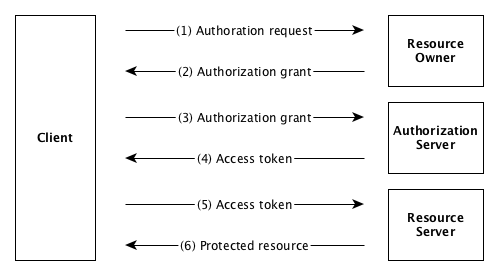
\includegraphics[scale=0.8]{pics/Ablauf_OAuth2.png}
    \caption{Ablauf des OAuth 2.0 Protokolls}
    \small \url{https://miro.medium.com/max/1400/1*1McvnvrW6wh37ECYpmTSxw.png} 
    \label{fig:impl:OAuth2Protocoll}
\end{figure}

Diese Grafik beschreibt den Weg, den der Client geht, um sich die Rechte auf die bestimmte Ressource (z.B. Veröffentlichung eines Beitrags) zu sichern. \\*
Wie man an der Grafik erkennen kann, übergibt OAuth 2.0 beim Kommunizieren nicht direkt den Benutzernamen und das Passwort des Benutzers. 
Als Kommunikationsgrundlage dient ein Access-Token, dieser kann jeder Zeit ungültig gemacht werden, somit verliert der Client auch die Rechte auf die Ressource. \cite{KeycloakCodeCentric}

\subsection{OpenID Connect (OIDC)}
Mit Keycloak ist es ebenfalls möglich OIDC umzusetzen bzw. zu benutzen. \\*
OpenID Connect ist ein Authentifizierungs- und Autorisierungsprotokoll, das im Februar 2014 von der OpenID Foundation veröffentlicht wurde.
Es erweitert die Funktionalität von OAuth 2.0 und benutzt dazu auch JWT (JSON Web Tokens). \\*
OpenId Connect soll die zentrale Stelle zur Verwaltung eines Benutzerprofils sein. Somit läuft auch jeder Authentifizierungsprozess über diesen ab.
Der Browser soll quasi die zentrale Komponente im Internet darstellen und jede Website benutzt die selbe OIDC Authentifizierung. Somit bleiben einem mehrere Benutzeraccounts erspart. \cite{KeycloakCodeCentric}
\pagebreak

\subsubsection{Ablauf von OIDC}
\begin{figure}[htp]
    \centering
    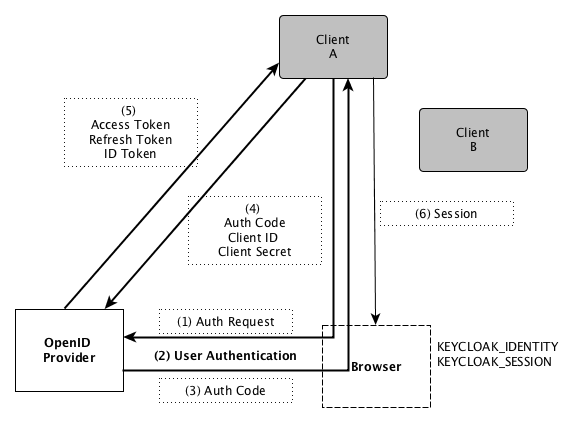
\includegraphics[scale=0.6]{pics/Ablauf_OIDC.png}
    \caption{Ablauf des OIDC Protokolls}
    \small \url{https://blog.codecentric.de/files/2016/08/openidconnect1.png} 
    \label{fig:impl:OIDCProtocoll}
\end{figure}

Der Browser leitet den Benutzer anfangs zum OpenID Provider hin. Der Benutzer authentifiziert sich dann beispielsweise mit Name und Passwort .
Danach bekommt der Client einen Auth-Code, dieser wird dann zum Access, Identity und Refresh Token umgewandelt.
Der Client wird durch Keycloak verifiziert, indem er vorher bei Keycloak mit einem Secret und einer ID konfiguriert wurde. Dies verhindert, dass kein willkürlicher Client diese Information erhalten kann.
In dem ganzen Prozess muss aber sichergestellt sein, dass jede Komponente das Secret sicher bewahren kann.
Zu allerletzt setzt der Browser dann die Session vom Benutzer und diese bleibt auch. \cite{KeycloakCodeCentric}

\subsubsection{Unterschied zu OAuth 2.0}
Der initiale Ablauf ähnelt dem von OAuth 2.0, doch der große Unterschied liegt in den Tokens.
Bei OIDC wird ein JWT (Json Web Token) übergeben. Dieser enthält Informationen zur Identität und zu den Attributen des Benutzers.
Diese können dann von der Applikation benutzt werden. \cite{KeycloakCodeCentric}


\subsection{Features}
\subsubsection{Multiple Protocols Support}
Gerade unterstützt Keycloak drei verschiedene Authentifizierungsprotokolle: OpenID Connect, OAuth 2.0 und SAML 2.0 \cite{KeyCloakDZone}
\subsubsection{SSO (Single Sign-On)}
\hyperref[sec:SSO]{Siehe hier}
\subsubsection{Admin Konsole}
Keycloak stellt eine web-basiertes Interface zur Verfügung, wo der Admin seine Konfigurationen intuitiv vornehmen kann. \cite{KeyCloakDZone}
\subsubsection{User Identity und Accesses}
\hyperref[sec:IAM]{Siehe hier}
\subsubsection{External Identity Source Sync}
Wenn man ein eigene User-Datenbank  hat, kann man diese mit Keycloak verbinden und synchronisieren. Standardmäßig unterstützt es LDAP und Active Directory, diese sind aber
erweiterbar durch selbstgeschriebene Extensions. Dies kann man mit der Keycloak User-Storage API machen. Es garantiert aber nicht, dass Keycloak alle Funktionen aufweist,
die auch die Datenbank hat. \cite{KeyCloakDZone}
\subsubsection{Identity Brokering}
Keycloak kann auch als Proxy zwischen den Usern und einem oder mehreren externen Identity Provider fungieren. Diese können im Admin Panel editiert werden. \cite{KeyCloakDZone}
\subsubsection{Social Identity Providers}
Zusätzlich erlaubt Keycloak die Benutzung von Social Identity Providern. Es hat eine eingebaute Unterstützung für Google, Twitter, Facebook, Stack Overflow, diese müssen aber 
im Admin Panel manuell konfiguriert werden. Die volle Liste der kompatiblen Social Identity Provider kann in der Keycloak Dokumentation gefunden werden. \cite{KeyCloakDZone}
\subsubsection{Anpassung von Seiten}
Keycloak erlaubt eine Anpassung aller Seiten, die dem User angezeigt werden (z.B. Login-Page). Die Seiten sind im FTL Format geschrieben, somit kann man klassisches HTML und CSS zum Editieren verwenden.
Auch Javascript steht zur Verfügung, damit ist der Anpassungsspielraum sehr groß. \cite{KeyCloakDZone}
\pagebreak

\subsection{Funktionsweise}
\begin{figure}[htp]
    \centering
    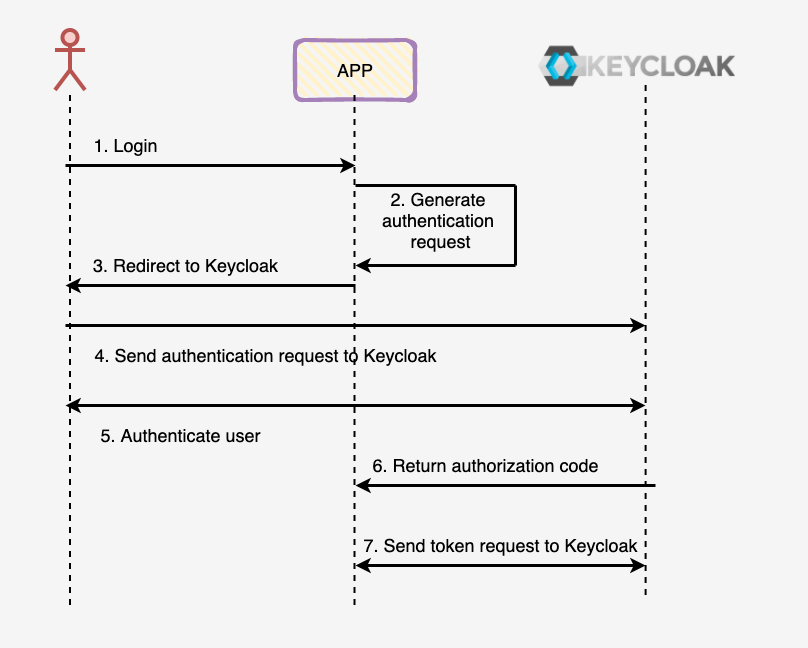
\includegraphics[scale=0.55]{pics/Keycloak-Funktionsweise2.png}
    \caption{Keycloak Funktionsweise}
    \small \url{https://miro.medium.com/max/1400/1*1McvnvrW6wh37ECYpmTSxw.png}
    \label{fig:impl:KeycloakFunc}
\end{figure}

Keycloak speichert sich einen Public Link der Applikation. Wenn dieser Link von einem User geöffnet wird, leitet Keycloak diesen zu einer Keycloak Authentication Page weiter.
Nach dem erfolgreichen Einloggen leitet Keycloak den User dann zu dem eigentlich gewünschtem Link weiter und gibt einen Token mit Zeitstempel mit.
Die Applikation kann dann den Token verwenden um den User und seine Rechte zu identifizieren. \cite{KeycloakMakeIT} \\*
\textbf{Bei der Funktionsweise sind wichtige Begriffe nötig:}

\subsubsection{Realm}
Ein Realm kann man sich als Vermieter vorstellen, der einen Bereich zur Verfügung stellt. Dieser sogenannte Realm ist vollkommen isoliert (im Sinne von Usern, Konfigurationen, Rollen, etc.)
von anderen Realms. \\* Aus diesem Grund kann man einen internen Realm für z.B. Mitarbeiter machen und einen externen für z.B. Kunden. Somit sind die beiden von einander getrennt. \cite{KeyCloakCodex}

\subsubsection{Client}
Clients sind die Anwendungen, die eine Authentifizierung von Keycloak fordern, also z.B. eine Webapp. Diese können aber auch mobile oder native Applikationen sein.
Sie können jeder Servicetyp sein wie REST API's, gRPC oder WebSockets, die nur eine simple Authentifizierung und Rollenvergabe mittels Access Tokens benötigen. \cite{KeyCloakCodex}

\subsubsection{Rollen}
Eine Rolle repräsentiert eine Rolle in der Organisation bzw. in der Applikation. Ein User kann z.B. eine Admin-Rolle bekommen und somit alles an der Applikation konfigurieren.
Wenn man dies nicht will kann man Rollen und deren Spielraum eingrenzen, sodass die Applikation nicht willkürlich verändert wird. \\*
Keycloak unterstützt ebenfalls zusammengesetzte Rollen. Diese Funktion sollte man aber vorsichtig behandeln, da diese die Komplexität der Applikation erhöht und diese somit schwerer zu pflegen ist. \cite{KeyCloakCodex}

\subsubsection{User}
Der User ist der eigentliche Benutzer der Applikation. Dieser kann dementsprechend zu einem Realm gehören und seine eigenen Rechte haben.
Dieser identifiziert sich durch den Client und seine Rollen im Realm werden der Applikation mitgegeben.


\section{Oracle Datenbank}
\author{David Ignjatovic}
Oracle Database ist ein relationales Datenbankmanagementsystem, auch genannt RDBMS, welches von der Firma Oracle hergestellt worden ist. 
Oracle ist einer der bekanntesten und auch meist verwendeten Datenbanken. Die Firma Oracle wurde am 17. August 1977 Lawrence Joseph Ellison in der Bronx, New York City, gegründet.
Die erste Version von Oracle Database kam 1979 auf den Markt. \cite{OracleDB} \\*

Die Oracle Database nutzt wie die meisten relationale Datenbanken, SQL als Programmiersprache (Structured Query Language).
SQL wird in der Oracle Database verwendet, um Aktionen durchzuführen, Datenbankstrukturen zu schaffen, Datensätze zu verwalten oder enthaltene Daten abzurufen. 
PL/SQL, welche eine Oracle-eige Sprache ist, ist wiederum eng verknüpft mit SQL und bietet die Möglichkeit, SQL um Oracle-Programmiererweiterungen zu ergänzen. 
Oracle verwendet Zeilen- und Spaltentabellen zur Strukturierung der Datenbanken, in denen Datenpunkte über Attribute verbunden sind \cite{OracleDB} \\*

Wichtige Oracle-Database-Werkzeuge währen Oracle SQL Developer und Oracle Data Modeler. \\*

Mit dem Oracle SQL Developer kann man leicht Datenbankabfragen auf einer graphischen Oberfläche tätigen. Noch dazu kann man PL/SQL Prozeduren erstellen oder generieren lassen.
Der Oracle Data Modeler wird hauptsächlich zum Erstellen von Datenbankmodellen oder Entity-Relationship-Modellen verwendet. Zum Schluss hat man dann die Möglichkeit ein Skript 
zu generieren welches dann alle Tabellen erstellt und auch die dazu modellierten Beziehungen erstellt.

\section{SQL}
\author{David Ignjatovic}

SQL steht für Structured Query Language und ist eine Datenbanksprache zur Erstellung von Datenbankstrukturen in relationalen Datenbanken 
aber auch zum Bearbeiten und Abfragen von Daten. Die Datenbanksprache basiert auf der relationalen Algebra. Die Syntax ist einfach und an die englische Sprach angelehnt. 

Mit Abfragen werden Daten in einer Datenbank abgerufen. \cite{SQL}

\subsection{SQL - Select}

Der Select Befehl in der Datenbanksprache, ist sozusagen der Grundstein für SQL-Abfragen.  \\*

\begin{lstlisting}[language=SQL,caption=Sql Select,label=lst:impl:foo]
SELECT t.Spaltenname1, t.Spaltenname2 FROM Tabellenname t
\end{lstlisting}

Wenn man den Select Befehl mit einem \textbf{WHERE} erweiter, kann man die Datenbank abfrage umso genauer gestallten. Es werden sommit nur spezielle Daten abgefragt. \\*

\begin{lstlisting}[language=SQL,caption=Sql Select Where,label=lst:impl:foo]
SELECT t.Spaltenname1, t.Spaltenname2 FROM Tabellenname t WHERE t.Spaltenname1 = 1
\end{lstlisting}


Die wichtigsten SQL-Comands lauten:
\begin{itemize}
  \item SELECT - extrahiert Daten aus der Datenbank
  \item UPDATE - aktualisiert Daten in der Datenbank
  \item DELETE - löscht Daten aus einer Datenbank
  \item INSERT INTO - fügt neue Daten in die Datenbank ein
  \item CREATE DATABASE - erstellt eine neue Datenbank
  \item ALTER DATABASE - modifizert eine Datenbank
  \item CREATE TABLE - erstelt eine neue Tabelle
  \item ALTER TABLE - modifiziert eine Tabelle
  \item DROP TABLE - löscht eine Tabelle
  \item CREATE INDEX - erstellt einen Index
  \item DROP INDEX - löscht den Index
\end{itemize}

\section{Vue.js}
\author{Benjamin Besic}
Vue.js ist ein JavaScript-Webframework, das zum Erstellen von Single-Page-Webanwendungen dient. 
Es wurde von einem kleinen Team im Jahre 2014 entwickelt mit dem ursprünglichem Autor Evan You.\\* Vue ist relativ neu und die große Stärke
von Vue ist die einfache Lernkurve, die Vielseitigkeit und die Leichtgewichtigkeit. Man benötigt Kenntnisse in JavaScript, HTML, CSS und schon kann man loslegen
mit deren ausführlich dokumentierten Guide\cite{VueGuide}. \cite{VueWissen} \cite{VueWiki}\\*

\subsection{Vue Funktionsweise}

\subsubsection{Model-View-Viewmodel (MVVM) Pattern }
Vue.js benutzt das MVVM Pattern. Das Pattern trennt die Darstellung von der Logik der Benutzer-UI's.
Dazu ist ein Datenbindungsmechanismus vorausgesetzt. Dadurch können sich Entwickler und Interfacedesigner trennen und ihre Aufgaben im Projekt 
aufteilen. \\*
Dieses Pattern wurde 2005 von John Gossman veröffentlicht. \cite{MVVM}

\begin{figure}[htp]
    \centering
    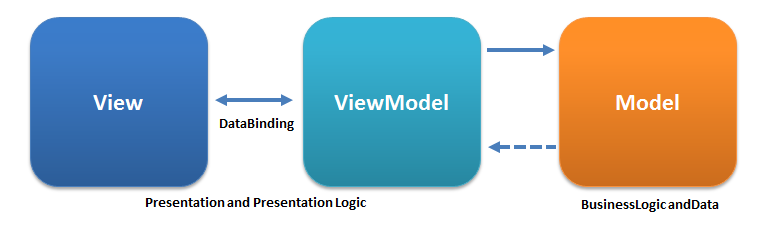
\includegraphics[scale=0.7]{pics/MVVMPattern.png}
    \caption{Darstellung von Branches in einem Repository}
        \small \url{https://upload.wikimedia.org/wikipedia/commons/8/87/MVVMPattern.png}
    \label{fig:impl:MVVM}
\end{figure}

\begin{itemize}
    \item \textbf{View:} Enthält alle Elemente die durch die Benutzeroberfläche angezeigt werden. Es bindet sich an das ViewModel, welches die Eigenschaften der View bestimmt.
    \item \textbf{ViewModel:} Es enthält die Logik des UI's. Es tauscht sich mit dem Model aus und benützt seine Methoden und Dienste. Gleichzeitig
          gibt es der View Eigenschaften, die dem Model entsprechen. Es bindet Daten mit der View und sich selbst (DataBinding).
    \item \textbf{Model:} Diese Schicht enthält alle Daten die der Benutzer manipuliert oder aufruft. Es enthält die gesamte Geschäftslogik.\cite{MVVM}
\end{itemize}

\clearpage

\subsubsection{Vue Instance}

Jede Vue Applikation beginnt mit der Erstellung einer Vue Instanz.

\begin{lstlisting}[language=JavaScript,caption=Vue Instanz,label=lst:impl:foo]
    var vm = new Vue({
        // options
    }) 
\end{lstlisting}

Die Variable vm steht für ViewModel, was unsere Vue Instanz darstellt. Man kann jeder Instanz Optionen zuweisen, um sie zu konfigurieren.
Diese Instanz wird auch als Root Instanz bezeichnet und bildet den Stamm eines Baumes mit Komponenten. 

\begin{figure}[htp]
    \centering
    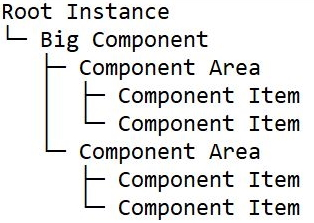
\includegraphics[scale=1]{pics/RootComponentTree.JPG}
    \caption{Der Stammbaum einer Root Instanz}
    \label{fig:impl:RootComponentTree}
\end{figure}
Zu einer Instanz gehört auch der data-Bereich. Dieser beherbergt alle Properties einer
Instanz und diese Properties reagieren auf Veränderungen von Werten. Noch dazu kann jede Instanz Methoden haben. \\*
Jede Instanz hat auch seine Lifecycle Hooks, dies sind Methoden, die zu bestimmten Zeitpunkten einer Instanz ausgeführt werden. \cite{VueGuideInstance}
Diese sind:
\begin{itemize}
    \item \textbf{created}
    \item \textbf{mounted}          
    \item \textbf{updated} 
    \item \textbf{destroyed} 
\end{itemize}
\clearpage

\subsubsection{Lifecycle Diagram}
Das Diagramm hier stellt den Ablauf einer Erstellung einer neuen Vue Instanz dar.

\begin{figure}[htp]
    \centering
    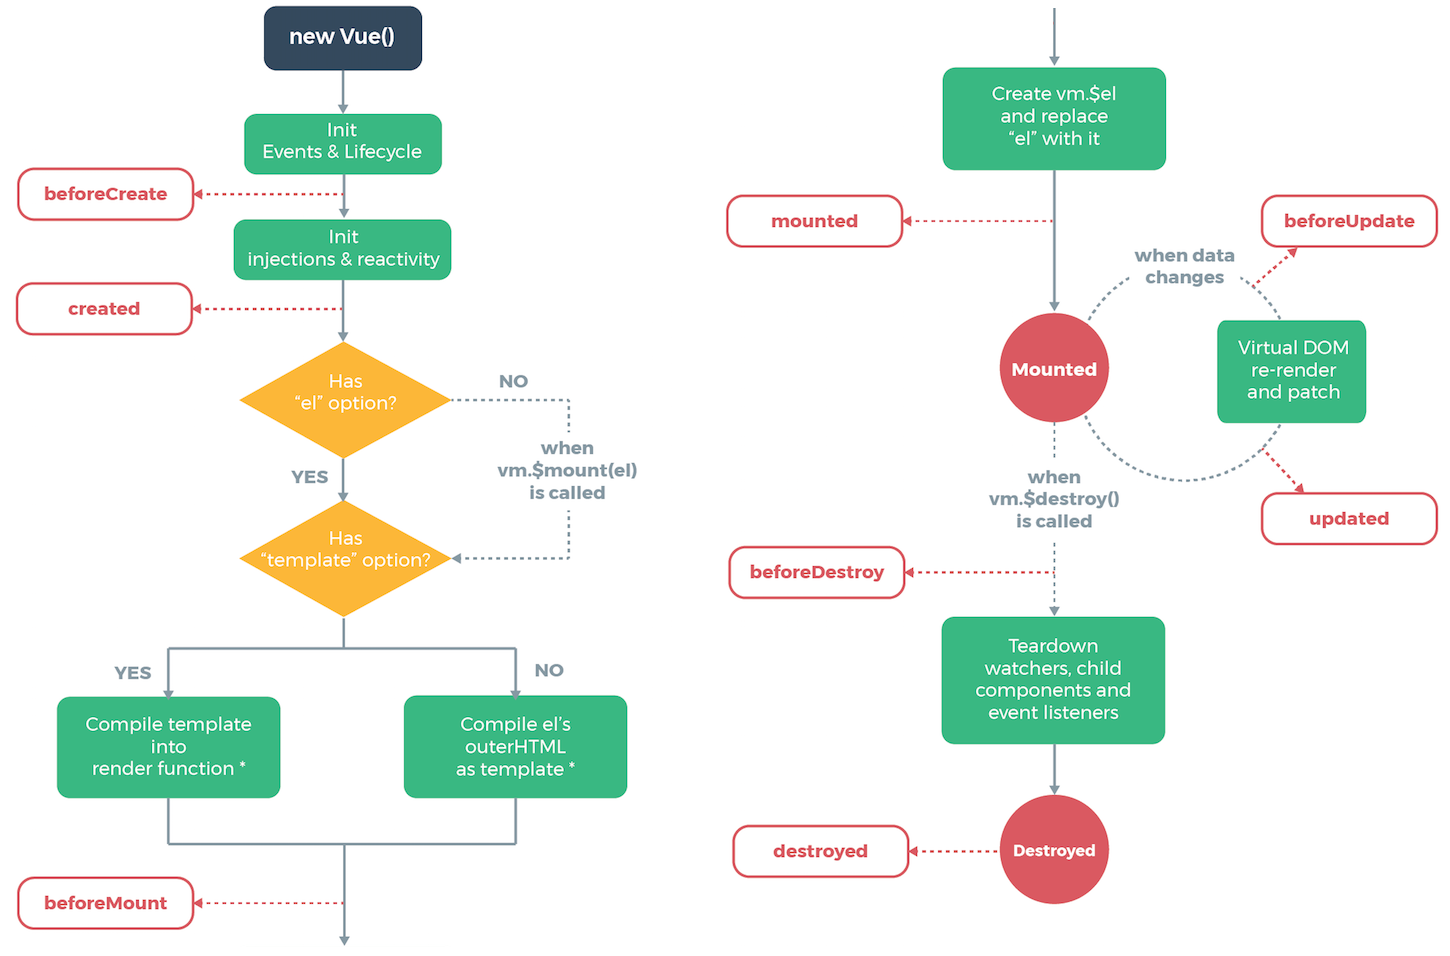
\includegraphics[scale=0.3]{pics/VueInstanceLifeCycle.png}
    \caption{Diagramm des Ablaufs einer Vue Instanz}
        \small \url{https://www.oreilly.com/library/view/full-stack-vuejs-2/9781788299589/assets/9f308e86-bbbe-489c-9f93-06abe2675081.png}
    \label{fig:impl:VueInstanceLifeCycle}
\end{figure}


\subsubsection{Vue Components}
Komponenten sind wiederverwendbare Vue Instanzen mit einem eigenen Namen. Diese Komponenten können mittels HTML-Tags in anderen Komponenten verwendet werden.
Eine Vue.js Seite ist meistens in mehrere Komponenten aufgeteilt, um größere Bereiche auf der Seite zu trennen und übersichtlicher zu gestalten. Diese können miteinander 
kommunizieren und Daten austauschen, um z.B. Daten, die ständig verändert werden ordentlich darzustellen.\cite{VueGuideComponents} \\*
\begin{figure}[htp]
    \centering
    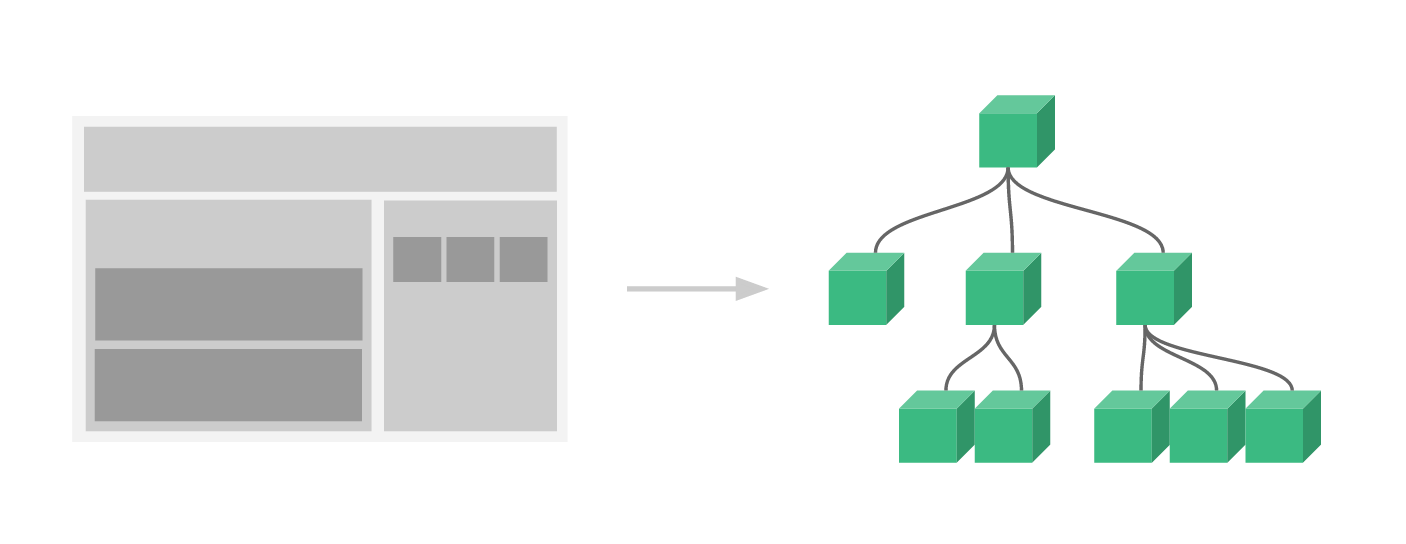
\includegraphics[scale=0.3]{pics/NestedComponentsTree.png}
    \caption{Darstellung von vernetzten Komponenten innerhalb einer Webpage}
        \small \url{https://vuejs.org/images/components.png?_sw-precache=b5c08269dfc26ae6d7db3801e9efd296}
    \label{fig:impl:NestedComponentsTree}
\end{figure}
Die folgende Grafik veranschaulicht den Component Tree, der zeigt, wie die Single-Page Anwendung umgesetzt ist. 
Die grünen Boxen zeigen die miteinander vernetzten Komponenten, jeder Komponent kann mehrere Unterkomponenten haben, je nach Einteilung der Webseite.
\subsection{Angular vs. Vue}
\subsubsection{Marktstatistik}
\textbf{Angular:}
\begin{itemize}
    \item Angular wird eher für Seiten benutzt mit hohen Aufrufzahlen \cite{AngularUsage}
    \item Nachdem was bekannt ist, benutzen unter 0.4\% aller Webseiten Angular \cite{UsageJSLibs}   
    \item Angular wird von 22.96\% Entwicklern weltweit verwendet \cite{AngVsVueSIM}
\end{itemize}

\textbf{Vue:}
\begin{itemize}
    \item Es gibt mehr als 2.071.882 Millionen Webseiten, die Vue benutzen
    \item Der Marktanteil von Vue bei Webseiten mit hohen Aufrufzahlen, beträgt nicht mehr als 0.8\% \cite{AngVsVueSIM}       
\end{itemize}
\subsubsection{Vor- und Nachteile}
Von der Lernkurve her ist Vue deutlich im Vorteil, da es einfacher zu verstehen ist als Angular. Angular benötigt viel Einarbeitungszeit, bis man die Funktionsweise
verstanden hat. Angular ist eher für umfangreiche Projekte gedacht, währenddessen Vue auf geringe Größe und hohe Performance abzielt. \\*
In Angular sind die Logik und das Aussehen strikt getrennt, währenddessen in Vue alles in einem File zu finden ist und mehr an HTML erinnert durch die Scripts, die man schreibt.
Ein Vorteil von Angular ist die Implementierung von Typescript, was eine Weiterentwicklung von JavaScript ist, die versucht die Macken von JavaScript zu verbessern.\\* 
Was noch zu erwägen ist ist, dass Angular bei Entwicklern weiter verbreitet ist als Vue und es oft Features oder Plugins gibt, die in Angular selbstverständlich sind, aber in Vue nicht aufzufinden sind.
Dies sollte sich aber im Laufe der Zeit verbessern. \\*  Generell kann man sagen, dass das Programmieren mit Angular eher and die Programmierung mit Java erinnert mit den Objekten, Abhängigkeiten,
Konstruktoren und so weiter. Während Vue an das Programmieren von Websites mittels HTML und JavaScript erinnert. \cite{AngVsVueHOST}
\subsubsection{Warum Vue?}
Unsere Entscheidung Vue zu nehmen ist einerseits von der Firma beeinflusst worden, da sie es vorgeschlagen haben und es bei ihnen das gängige Framework ist.\\*
Andere Faktoren waren noch, dass wir Angular in der Schule oft verwendet haben und wollten durch Vue eine andere Methode ausprobieren, um Webanwendungen zu erstellen.
Vue ist die bessere Wahl für den Umfang unserer Webanwendung gewesen und die bessere Performance in Vue ist wichtig, damit die Bestellungen reibungslos ablaufen können im Echtbetrieb.

\section{HTML}
\author{Benjamin Besic}
HTML genannt HyperText Markup Language, ist eine einheitliche, textbasierte Auszeichnungssprache für Webdokumente. HTML definiert ganz allgemein gesehen die Struktur eines Dokuments. 
Am 13.März 1989 wurde am CERN in Genf das Konzept HTML von Tim Berners-Lee vorgeschlagen, um eine einheitliche Methode zu finden Dokumente öffentlich zu übermitteln. Seitdem ist HTML  einer Grundbausteine des World Wide Webs geworden. \\*
HTML basiert auf sogenannten Tags, die verschiedene Inhalte auf der Website definieren sollten. Diese basieren auf einer bestimmten Syntax, um das Schreiben zu vereinheitlichen. \\*
Es ist im Grunde eigentlich keine klassische Programmiersprache, sondern eine statische Sprache, die zur Definierung benutzt wird, auch genannt deklarative Programmiersprache.  
Das HTML Gerüst wird von einem Browser eingelesen und dieser generiert dann auf der Basis des HTML Files eine Website. \cite{HTMLTut} \cite{HTMLSeoKueche}

\begin{lstlisting}[language=HTML,caption=HTML File Grundgerüst,label=lst:impl:foo]
<!DOCTYPE html>
<html>
    <head>
        <title> Titel der Webseite </title>
    </head>
    <body>
        <h1> Ueberschrift </h1>
    </body>
</html>
\end{lstlisting}

Wie man im Beispiel sieht, gibt es bei Tags einen Anfang und ein Ende und der Inhalt dazwischen wird dargestellt.
Es gibt auch Tags ohne Ende, sogenannte inhaltsleere Tags.
Doch HTML wird meist nie allein verwendet, erst in der Kombination mit CSS, Bootstrap und JavaScript kann man eine gute Website erstellen.

\section{CSS}
\author{Benjamin Besic}
CSS (Cascading Style Sheets) ist die Sprache, die benutzt wird, um eine HTML Seite visuell zu gestalten. CSS ist wie HTML keine Programmiersprache, sie wurde dafür entwickelt um das Aussehen von HTML Seiten einheitlich zu verändern.\\*
Eine CSS-Datei wird durch einen Tag mit dem zugehörigen HTML Dokument verbunden und dadurch werden die Änderungen angewendet. \cite{CSSMozilla}

\begin{figure}[htp]
    \centering
    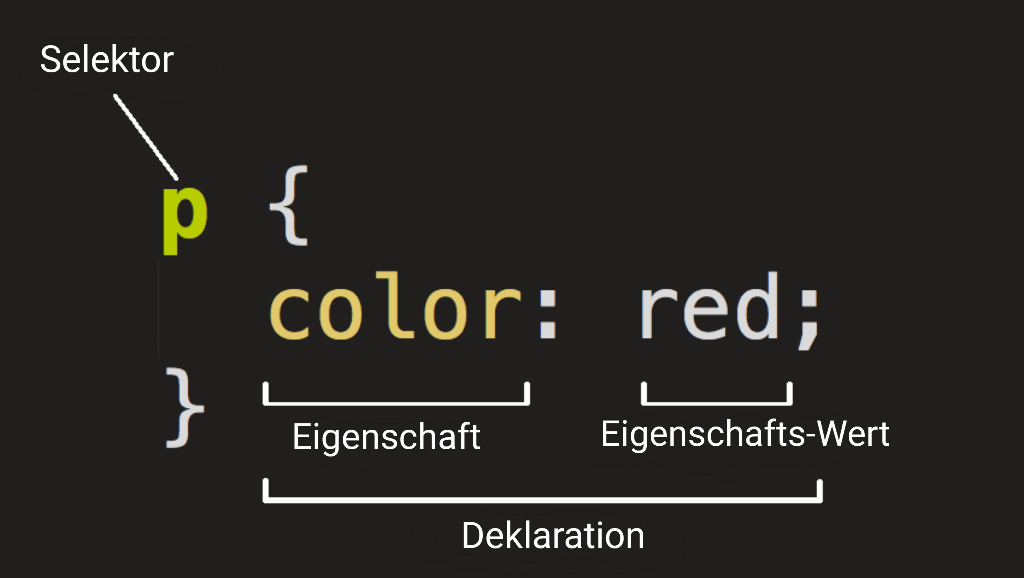
\includegraphics[scale=0.3]{pics/CSSRegel.png}
    \caption{Aufbau einer CSS-Regel}
        \small \url{https://media.prod.mdn.mozit.cloud/attachments/2017/09/27/15467/3889d04d90c10b27e863c6850d588c43/css-example.png}
    \label{fig:impl:CSSRule}
\end{figure}

Die Struktur von CSS-Dateien wird durch Regeln beschrieben. Jede Regel hat einen Selektor, der auf ein zugehöriges HTML Tag zugreift.
Innerhalb der Deklaration wird dann der Wert einer bestimmten Eigenschaft gesetzt (mehrere Eigenschaften sind möglich).
Es gibt eine große Auswahl von Eigenschaften wie z.B.: Schriftfarbe, Textart, Positionierung, etc. \cite{CSSMozilla}

\section{JavaScript}
\author{Benjamin Besic}
JavaScript ist eine leichtgewichtige Skriptsprache, die 1995 vom Softwareunternehmen Netscape entwickelt worden ist, um die Möglichkeiten von HTML und CSS zu erweitern.
Bekannt ist sie hauptsächlich als Sprache für Webseiten geworden, jedoch wird sie auch in vielen Umgebungen außerhalb des Browsers oft benutzt, wie z.B. Servern. 
\\* Sie unterstützt objektorientierte, imperative als auch deklarative Programmierung (funktionales Programmieren). JavaScript folgt dem Standard ECMAScript, welchen alle Browser unterstützen. 
JavaScript dient dazu auf Webseiten Benutzerinteraktionen auszuwerten, Inhalte zu verändern, nachzuladen oder zu generieren.  \\*
Jedoch sollte man JavaScript nicht mit der Programmiersprache Java verwechseln. Beide sind verschiedene Handelsmarken der Firma Oracle und ähneln einander höchstens, was die Syntax betrifft.
\cite{JSWiki} \cite{JSMozilla}
\section{JSON Web Token (JWT)}
\author{Benjamin Besic}
JSON Web Token ist ein nach RFC 7519 genormter Standard, um Daten sicher zwischen zwei Parteien auszutauschen. Es wird in der Form eines JSON-Objektes übertragen.
Die Information, die der Token enthält kann verifiziert werden, weil es eine digitale Unterschrift enthält. Der Token selbst kann entweder mit einem geheimen Schlüssel (HMAC-Algorithmus) oder einem private/public Schlüsselpaar (RSA oder ECDSA) verschlüsselt werden.\\*
Beliebte Anwendungsfälle des Tokens sind Authentifizierung und Datenaustausch. Der Token selbst enthält Informationen über den Absender und ob er die nötigen Zugriffsrechte hat.
\cite{JWTIO} \cite{JWTIONOS}
\subsection{Aufbau eines JWT}
Ein signierter JWT besteht aus 3 Teilen, getrennt durch einen Punkt. Jeder dieser Teile wird mit Base64 kodiert. \\*
Jeder JWT hat auch eine Gültigkeitsdauer, wenn diese abgelaufen ist, gilt ein Token als ungültig.
\clearpage
\begin{figure}[htp]
    \centering
    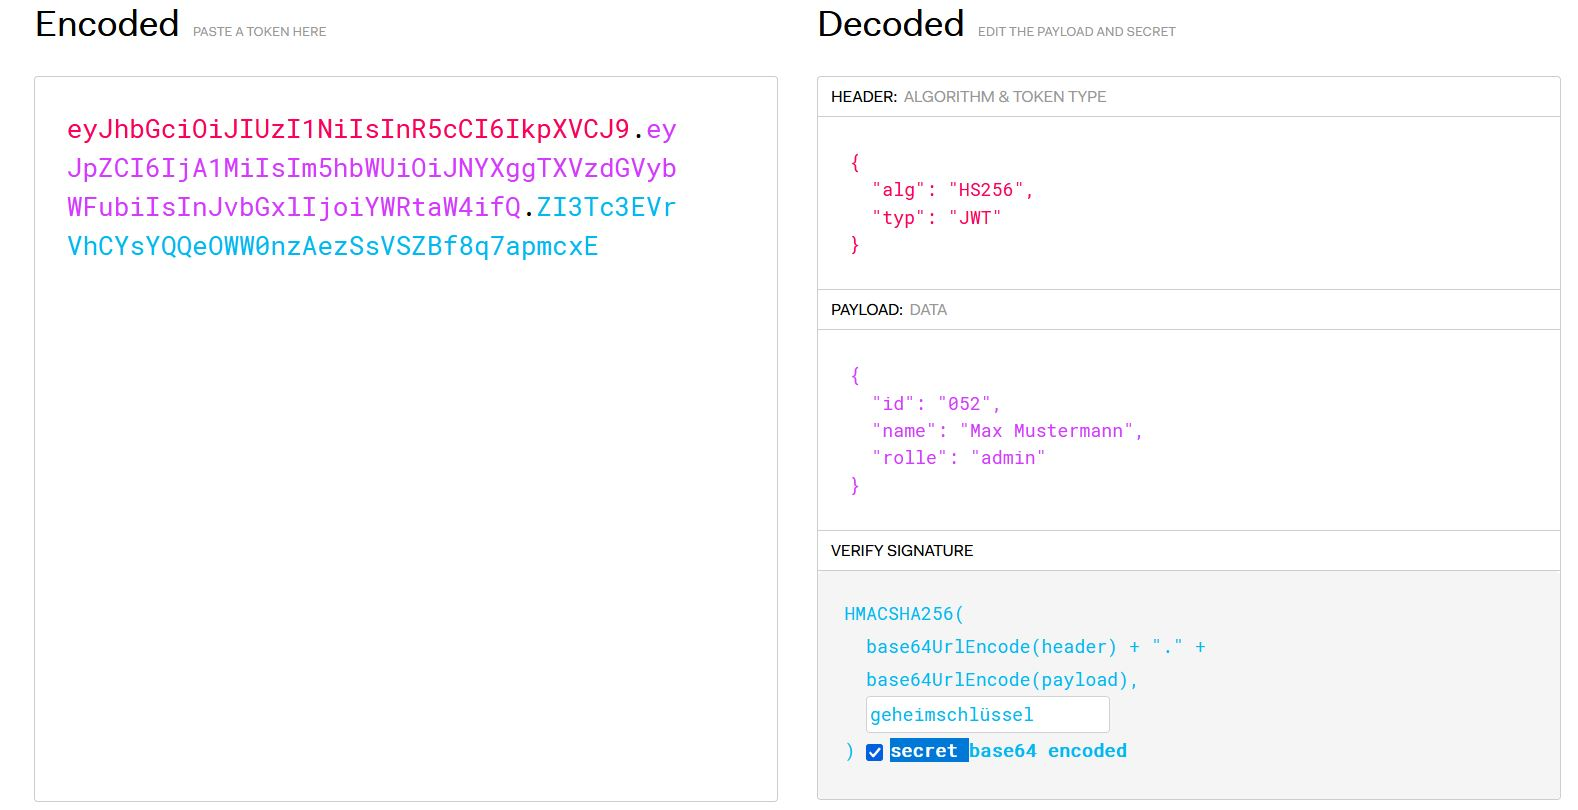
\includegraphics[scale=0.4]{pics/JWT.JPG}
    \caption{Aufbau eines JSON Web Tokens (Ausschnitt von jwt.io)}
        \small \url{https://jwt.io/}
    \label{fig:impl:JWT}
\end{figure}

\subsubsection{Header}
Der Header besteht meist aus zwei Teilen und liefert Informationen über den Typ des Tokens und den verwendeten Signatur- bzw. Verschlüsselungsalgorithmus.
\begin{itemize}
    \item Der ``typ''-Wert beschreibt den IANA Medientypen des Tokens, oft wird ``application/jwt'' verwendet.
    \item Der ``alg''-Wert gibt an welcher Algorithmus zum Signieren des Tokens verwendet wurde. Es ist auch möglich keine Verschlüsselung anzugeben, was jedoch nicht zu empfehlen ist. \cite{JWTIONOS}     
\end{itemize}
\subsubsection{Payload}
Der Payload ist der Teil des Tokens, der die tatsächlichen Daten bzw. Informationen enthält, die übermittelt werden sollen.
Sie werden als Key-/Value-Paare bereitgestellt, diese Werte werden bei JWT als Claims bezeichnet. \cite{JWTIONOS}  Davon gibt es drei verschiedene Arten:
\begin{itemize}
    \item \textbf{Registrierte Claims} sind standardisiert und im JWT Claim Register festgelegt. Es wird empfohlen diese zu verwenden.
    \item \textbf{Öffentliche Claims} sind nach belieben definierbar.
    \item \textbf{Private Claims} sind für Informationen gedacht, die speziell auf die Anwendung angepasst sind wie z.B. "Benutzer-ID". \cite{JWTIONOS} 
\end{itemize}

\subsubsection{Signature}
Diese wird durch Base64-Kodierung des Headers, des Payloads und der angegebenen Signaturmethode erzeugt. Der Aufbau ist definiert nach dem RFC 7515 Standard, auch genannt JWS (JSON Web Signature).
Damit die Signatur funktioniert, muss man einen geheimen Schlüssel verwenden, der nur dem Ursprung bekannt ist. \cite{JWTIONOS} 

\subsection{Sicherungsverfahren}
\subsubsection{Keine Sicherung}
Wenn die Daten keiner Verschlüsselung bedürfen, kann im Header "none" angegeben werden. In diesem Fall wird keine Signatur generiert, dadurch fällt auch der Signature-Teil weg. \\*
Ohne Sicherung lässt sich die Nachricht nach einer Base64-Entschlüsselung klar und deutlich lesen. Der Absender oder ob die Nachricht im Laufe verändert worden ist, ist nicht mehr verifizierbar.\cite{JWTIONOS} 
\subsubsection{Signatur (JWS)}
Im Normalfall reicht es nur zu prüfen, ob die Daten vom richtigen Absender kommen und ob Veränderungen geschehen sind. Die JWS (JSON Web Signature) führt diese Überprüfungen aus. 
\\* Bei diesem Verfahren lässt sich die Payload nach Base64-Entschlüsselung klar und deutlich lesen. \cite{JWTIONOS}
\subsubsection{Signatur (JWS) und Verschlüsselung (JWE)}
Es ist möglich zusätzlich zum JWS noch eine JWE (JSON Web Encryption) zu benützen. JWE verschlüsselt den Inhalt des Payloads, diese werden danach mit JWS signiert.
Um die Inhalte dann zu entschlüsseln wird noch ein Kennwort oder ein privater Schlüssel angegeben. \\*
Damit ist der Absender verifiziert, die Nachricht authentisch und der Payload ist nicht lesbar nach einer Base64-Entschlüsselung. \cite{JWTIONOS}


\section{Progressive Web App(PWA)}
Webanwendung werden mit Hilfe von HTML, CSS und Javascript wntwickelt. 
Das in Verbindung mit dem Progressive Enhancement, was für die Lauffähigkeit einer Webseite in jedem Browser verantwortlich ist, wird eine PWA genannt. 

Der Service-Worker arbeitet mit HTTPS und führt konstant einen Web-Browser im Hintergrund.
Dank ihm hat die PWA Zugriff auf Caching und kann Offline verwendet werden. 
Weiter noch stellt der Service-Workerr die Funktionalität der Push-Notification bereit.  


Vorteile sind die Kostenreduktion in der Entwicklung da man nur eine PWA benötigt, die man auf Android, IOS und Windows benützen kann.
Weiters kann man die PWA so konfigurieren, dass sie wie eine echte Applikation ausschaut.


\section{Google Charts}
\cite{Google-Charts}
Google Charts ist eine leicht verwendbare Möglichkeit, Werte in verschiedenen Darstellungen anzuzeigen.
Es gibt 18 verschiedene Arten von Diagrammen. Aber die meist benützen sind:

\begin{itemize}
    \item Histogram
    \item Bar Charts
    \item Donut Chart
    \item Collumn Chart
    \item Pie Chart
    \item Area Chart
\end{itemize}
Zu jedem Diagramm gibt es auch eine \textit{options}-Variable, welche das modifizieren ermöglicht.
Man kann somit die Höhe, Breite, den Titel und die einzelnen Farben angeben.
\linebreak
Viele solcher Features sind kostenpflichtige Angelegenheiten. Google Charts sind kostenfrei.

\section{Jetpack Compose}
\cite{Jetpack-Compose}
\author{Bozidar Spasenovic}
Jetpack Compose ist seit Juli 2021 in der ersten stabilen Version verfügbar. Es ist ein "Werkzeugkasten" zum Bauen von Android Applikationen.
Es vereinfacht und beschleunigt den Anwendungsentwicklungsprozess. Da man mit wenig Code schnell viele Ansichten erstellen kann, ist die Fehlerqoute dementsprechend niedrig.
Man kann zwischen drei Ansichten auswählen, welche Code, Split oder Design wären. Diese vereinfachen parallele Arbeiten sehr. 
Die App wird aber nicht nach jeder Änderung neu gebaut, was wiederum die Schnelligkeit des Arbeiten beeinflusst. Damit die Applikation eine schöne Oberfläche hat, stellt
Jetpack Compose mehrere Themes zur Verfügung. Noch dazu kann man diese dann auch selbst konfigurieren, indem man Items hinzufügt oder löscht.
Jetbrains hat in Planung eine plattformübergreifendes Open-source Projekt zu starten, damit man Desktop Anwendungen genau so schnell und einfach erstellen kann. 

\subsection{Wichtig zu wissen!}
\cite{Jetpack-Compose-Docu}
Um mit Jetpack Compose coole Applikationen entwerfen zu können, muss man die Anfangsschritte verstanden haben.

\begin{itemize}
    \item Jetpack Compose wird mithilfe von \textit{Android Studio} programmiert.
    \item Jetpack Compose basiert 100 Prozent auf Kotlin. 
    \item Laufzeit und Speichernutzung der App verbessern.
\end{itemize}

\subsection{Applikationsgröße}
Jede Applikation benötigt Speicher. Aber wie schafft man es den Speicher einer App zu minimieren. 
Auf den Speicher haben Bibliotheken einen großen einfluss. 

\subsection{Applikationsbauzeit}
\cite{Jetpack-Compose-Build}
Man kann mit einem einfachem Kommando die \textit{Build Time} herausfinden.
\begin{lstlisting}
    ./gradlew --profile --offline --rerun-tasks --max-workers=4 assembleDebug
\end{lstlisting}

\begin{itemize}
    \item \textit{--profile} ermöglicht das Profilieren
    \item \textit{--offline} verweigert das benützen von Abhängigkeiten aus dem Internet
    \item \textit{--rerun-tasks} wird verwendet um \textit{Gradle} um alle Prozesse zu wiederholen
    \item \textit{--max-workers=4} beschreibt die Anzahl der parallelen Prozesse \cite{Gradle-Max-Worker}
    \item \textit{assembleDebug} erstellt eine \textit{debug.apk} von der App
\end{itemize}


\subsection{Entwurf}
Jeder Entwurf sollte schön und benutzerfreundlich ausschauen. Somit kann man mit \textit{Theming} ein solches erstellen.
Dazu verwendet man meistens \textit{Material Theming}. Natürlich kann man aber auch eigene Entwürfe erstellen und verwenden.
Um Daten anzeigen lassen zu können, sollte man sich mit dem Thema \textit{Data Binding} auseinander gesetzt haben.
Dazu kommen noch die die Möglichkeiten Animationen, Grafiken und Gästen in die App einzubauen.


\subsection{Data Binding}
Data Binding ist eine sehr wichtige Funktion im Programmieren mit einer Benutzeroberfläche. Es wird verwendet um das Backend 
zu informieren, falls sich ein Wert ändert. Durch das Data Binding kann man also Aktivitäten und Aktionen kontrollieren und ausnutzen.
Um eine Variable binden zu können, muss man \textit{mutableStateOf} benutzen. 


\pagebreak
\section{Kotlin}
\cite{Kotlin1}
\cite{Kotlin2}
\author{Bozidar Spasenovic}
Kotlin ist eine universelle und statisch typisierte Open-Source-Programmiersprache, die ursprünglich für die Java Virtual Machine und Android entwickelt wurde.
Es konzentriert sich auf Interoperabilität, Sicherheit, Übersichtlichkeit und Werkzeugunterstützung. Als build-script wird Gradle verwendet.

2017 wurde sie zu einer offiziellen Sprache zur Entwicklung von Android-Applikationen. Deswegen wird Kotlin auch Programmiersprache der Zukunft betitelt wenn man sie mit Java vergleicht.
Lambdafunktionen werden deutlich reduziert und somit auch leichter in der Praxis als in Java. 
Da Kotlin sehr kompatibel mit Java ist, können beim Testen die Frameworks und Bibliotheken von Java sehr weiterhelfen.  
Ursprünglich hat man den Kotlin Code in Bytecode übersetzt und diesen dann in der JVM laufen gelassen. 
Aber den Code kann man aber auch in Javascript umschreiben lassen und somit für Web Anwendungen verwenden.

Einer der Hauptvorteile von Kotlin sind die Unterstützungen für Multiplatform-Programmierung.
Die Felxibilität sowie die Vorteile der nativen Programmierung bleiben erhalten, es reduziert sich aber 
der Umfang des Schreibens sowie des Programmiercodes.


\subsection{Die Unterteilung der Multiplatform von Kotlin?}

Man unterteilt in drei Abschnitte, mit \textit{Common Kotlin} als Kern.

\begin{itemize}
    \item JVM Code mit Kotlin/JVM
    \item JS Code mit Kotlin/JS
    \item Native Code mit Kotlin/Native
\end{itemize}

Der Kern \textit{Common Kotlin} beinhaltet das  Nötigste für das Programmieren. Wie zum Beispiel wichtige Bibliotheken
und basis Tools.


\pagebreak

\section{XML}
\cite{XML1}
\cite{XML2}
\author{Bozidar Spasenovic}
XML steht für eXtensible Markup Language und ist ein textformbasiertes Datenformat.
Das Wort eXtensible heißt übersetzt erweiterbar und soll die Erweiterungsmöglichkeiten der Sprache beschreiben.
Sie wurde im Jahre 1996 entwickelt und wurde zwe Jahre später zum W3C-Standard. 
Sie ist sehr leicht einsetzbar in verschiedene Anwendungen da sie keine Lizenz benötigt.
Viele Tools heutzutage erleichtern aber auch die Bearbeitung von XML-Dateien.
Ein Vorteil ist, dass man die Daten im XML als Textformat abspeichert, was heißt das XML auch plattformunabhängig ist.
Wie in HTML, gibt es auch hier sogenannte Tags, die aber selbst zu kofigurieren sind. 
Der große Vorteil von XML ist das es sehr leicht lesbar ist, sowohl von Mensch als auch von Machine.
Es wird in Android verwendet um das Layout jeder Aktivität des Android zu entwerfen und erleichtert die Datenübertragung zwischen Anwendungen.




\section{Docker}
\author{Bozidar Spasenovic}
Docker ist eine in GO programmierte Softwareplattform, die den Prozess des Erstellens, Ausführens und Verwaltens von Apps umfasst.
Dies geschieht durch Virtualisierung des Betriebssystems, auf dem es installiert ist und ausgeführt wird. 
\subsection{Docker Compose}
\cite{Docker-Compose}
Compose ist ein Tool zum Definieren und Ausführen von Docker-Anwendungen mit mehreren Containern. 
Um Container ausführen zu können, werden compose-files geschrieben um Docker-Anwendungen zu starten.
Die Compose-File ist eine \textit{.YAML} File, in der die konfiguration statt findet. 
Anschließend erstellen und starten Sie mit einem einzigen Befehl alle Dienste aus Ihrer Konfiguration.


\subsection{Verwendung}

Man setzt die Umgebung der App mit einer Dockerfile.
Danach wird die \textit{docker-compose.yaml} file erstellt, welche die einzelnen Dienste startet.

Starten mit -> docker-compose up \linebreak
Killen/Beenden mit -> docker-compose down




\section{OKHttp}
\cite{OkHttp}
\author{Bozidar Spasenovic}
OkHttp ist ein HTTP-Client, der standardmäßig effizient ist.
Dank der HTTP/2-Unterstützung ist es möglich alle Anfragen an einen Host zu schicken. 
Response Caching hilft zur Vermeidung von wiederholten Anfragen.
\linebreak  
OkHttp hilft bei Verbindungsproblemen indem man alternative Adressen benutzt und unterstürzt weiters noch TLS-Funktionen.
Der Client wird sich lautlos von Verbindungsproblemen erholen, sprich er bleibt bei Verbindungsproblemen noch vorhanden.
\linebreak
Falls ein Dienst mehrere IP-Adressen verfügt, wird sich der Client automatisch alternative Adressen aussuchen und mit denen
die Aufrufe noch einmal versuchen.
Das braucht man häufig für IPv4 und IPv6, weil die in redundanten Rechenzentren behütet werden. 


Es kann so konfiguriert werden, dass es auf eine breite Konnektivität zurückgreift.
Der Client ist sehr gut für die Verwendung von blockierte synchrone und nicht blockierte asynchrone Aufrufe 

\subsection{Was braucht man wenn man OKHttp benutzen will?}
OkHttp funktioniert ab der Android 5.0 aufwärts und Java 8. 
Es hängt von Okio und der Kotlin Standardbibliothek ab.   

\subsubsection{Kotlin Standardbibliothek}
\cite{Kotlin-Standartbibliothek}
Damit man überhaupt mit Kotlin programmieren kann, bietet die Standartbibliothek \textit{kotlin-stdlib} viele Packages an.
Standartgemäß bietet diese die einzelnen Datentypen wie zum Beispiel:

\begin{itemize}
    \item String
    \item Char
    \item Boolean
    \item Int
    \item Any
    \item etc.
\end{itemize}

Mit den mitgelieferten Packages wie zum Beispiel kotlin.io kann man ganz übliche Input/Output Funktionen verwenden.
Mit dem Package kotlin.collection werden Schleifen zu Verfügung gestellt.

Wenn man die neueste Version von OkHttp sucht, ist man auf Maven Central genau richtig.
Diese fügt man dann im build.gradle file ein und nach einem neu laden des Scriptes kann man es auch schon verwenden.

\pagebreak

\section{Retrofit}
\cite{Retrofit}
\author{Bozidar Spasenovic}

Retrofit ist ein REST-Client für Java und Android.
Es wird verwendet, um Requests zu empfangen, senden, antworten und erstellen von HTTP-Anforderungen.
Noch dazu wird die IP-Adressen ausgewechselt, wenn eine Verbindung zu einem Webdienstfehler besteht.
Über einen REST-basierten Webdienst wird es sehr einfach Daten hochzuladen oder auch abzurufen. 

\subsection{Verwendung}
Wenn man Retrofit benützen möchte, muss man darauf achten immer eine \textit{HTTP}-Annotation über die jeweilige Methode
zu schreiben. Die verfügbaren Annptationen lauten:

\begin{itemize}
    \item HTTP
    \item GET
    \item POST
    \item PUT
    \item DELETE
    \item OPTIONS
    \item HEAD
\end{itemize}


Zu den Annotationen kann man natürlich einen zugehörigen Pfad der Methode angeben.

\textit{@POST("persons/person")}

Man kann auch jeweilige \textit{Query}-Parameter mitgeben.

\textit{@POST("persons/person?id=1")}

Um einen Body übergeben zu können, schreibt man vor dem Methodenparameter \textit{@Body}.

\textit{
@POST("person/new")
Call<Person> addPerson(@Body Person person);
}



\section{Gradle}
\cite{Gradle1}
\cite{Gradle2}
\author{Bozidar Spasenovic}
Gradle ist ein 2007 entwickeltes Build-Management-Automatisierungs-Tool, welches auf Java basiert.
Man kann es mit Apache Maven und Ant vergleichen.
Es hat die Flexibilität von Apache Ant und die simple Bedingungsmöglichkeit von Maven.
Der Unterschied zu den  Maven-Projektdefinitionen ist, dass man Gradle-Scripts gleich ausführen kann.
 Gradle unterstütz neben Java noch die Programmiersprachen Groovy und Kotlin.
DAG wird verwendet, um die Tasks in richtiger Reihenfolge zu dirigieren.
Heutzutage hat Gradle eine eigene Maschine für das Verwalten der einzelnen Abhängigkeiten, aber es begann mit Apache Ivy.
Seit Mitte 2013 ist Android hinzugekommen. Seitdem wurde das Tool weitgehend erweitert, um den Aufbau sogenannter „nativer“ Systeme zu unterstützen, welche nicht auf Java basieren.
Gradle wird von sehr großen Unternehmen verwendet wie zum Beispiel LinkedIn, Netflix, Adobe und vielen weiteren.

Inwiefern man das Gradle Script verändern möchte, kann man auswählen zwischen
\begin{itemize}
    \item Plugins
    \begin{figure}[htp]
        \author{Bozidar Spasenovic}
        \centering
        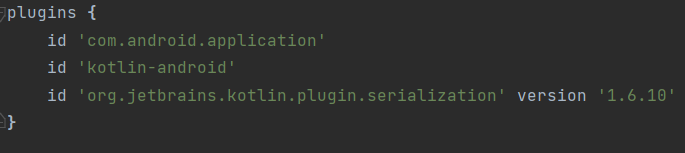
\includegraphics[scale=0.80]{pics/gradle-plugins.PNG}
        \caption{Gradle-Plugin}
        \label{fig:impl:gradle-plugin}
    \end{figure}   
    \item Default Android
    \begin{figure}[htp]
        \author{Bozidar Spasenovic}
        \centering
        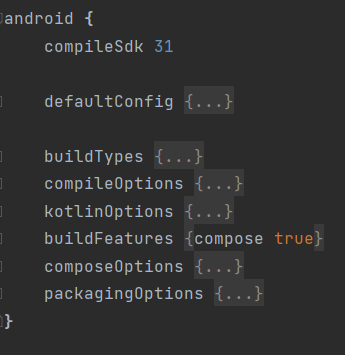
\includegraphics[scale=0.80]{pics/gradle-android.PNG}
        \caption{Gradle-Android}
        \label{fig:impl:gradle-android}
    \end{figure}   
    \item Dependencies
    \begin{figure}[htp]
        \author{Bozidar Spasenovic}
        \centering
        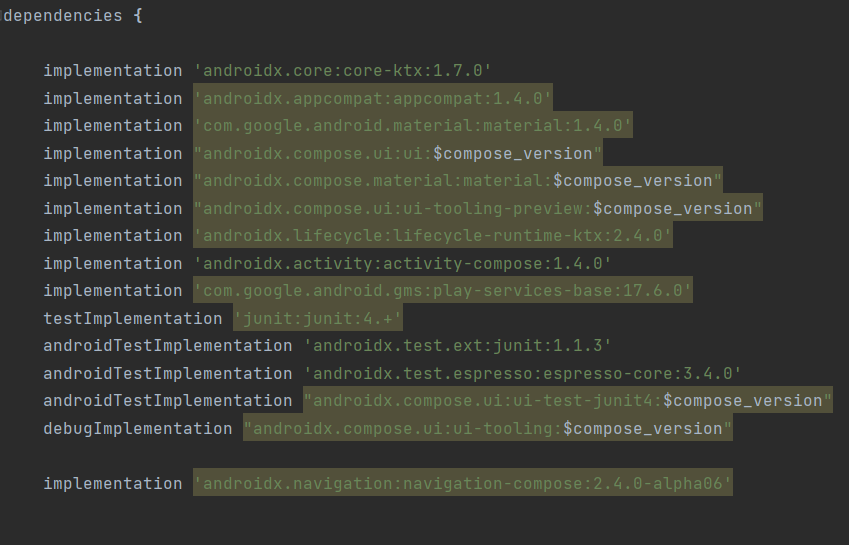
\includegraphics[scale=0.50]{pics/gradle-dependencies.PNG}
        \caption{Gradle-Dependencies}
        \label{fig:impl:gradle-Dependencies}
    \end{figure}   
\end{itemize}





\pagebreak



\section{Asciidoc}
\author{David Ignjatovic}

AsciiDoc ist ein Textformat, welcher hauptsächlich für Dokumentationen, Webpages, Blog und vieles mehr verwendet mit.
Da AsciiDoc ein plain-text Format ist und nicht wie die meisten Anwendungen für Textverarbeitungen Binärformate sind, wird es auch als Docs-as-Code bezeichnet.

AsciiDoc wurde entwickelt, um Dokument so zu schreiben als währen sie normale Textdokumente. Da das Design von AsciiDoc schon inkludiert ist,
muss man nicht einstellen wie die einzelnen Schriftgrößen für Überschriften sind. Somit ist man mit AsciDoc viel schneller als mit einer Anwendung,
welche in Binärform ist.

\section{Asciidoctor}
\author{David Ignjatovic}

Asciidoctor ist eine open source Textverarbeitung, welche AsciiDoc Text in Formate wie HTML 5, PDF und weiter, umwandelt.

Asciidoctor selbst ist in Ruby entwickelt worden. Um aber Asciidoctor zu verwenden braucht man kein Ruby. Mittels AsciidoctorJ
kann man ganz einfach Asciidoctor auf einer JVM ausführen.

\pagebreak

\section{Swagger}
\author{David Ignjatovic} 

Swagger ist ein Open-Source Werrkzeug welches verwendet wird um HTTP-Webservices zu entwerfen, dokumentierten aber auch zu benutzen. Um einen leichten überblick über seine 
ganzen Endpoints zu haben, wird Swagger verwendet, da es ganz schnell und einfach zum verwenden ist. \\*

Damit man Swagger in einem Quarkus Backend verwedet, muss mann in den Application.Properties folgende Zeile eintragen:

\textbf{quarkus.swagger-ui.always-include=true}

Die Sagger Page wird dann unter folgender URL abgerufen: 

\textbf{\textit{http://localhost:8080/q/swagger-ui/ }}

Wie schon erwähnt, kann man bei der Swagger Page alle Requests sehen die verwendet werden. 

\begin{figure}[htp]
    \author{David Ignjatovic}
    \centering
    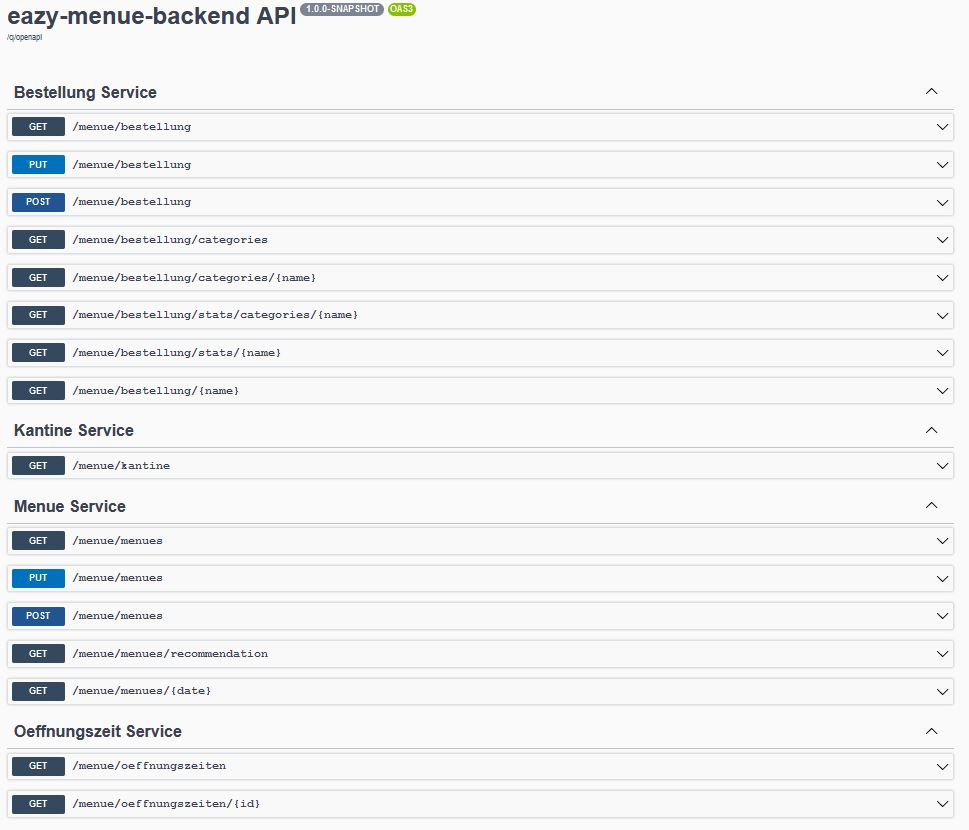
\includegraphics[scale=0.60]{pics/swagger.jpg}
    \caption{SwaggerUI}
    \label{fig:impl:swagger}
\end{figure}

Noch dazu kann man mit Swagger auch einzelne Data Transfer Objects veranschaulichen, welche in den Requests verwendet wird.

\begin{figure}[htp]
    \author{David Ignjatovic}
    \centering
    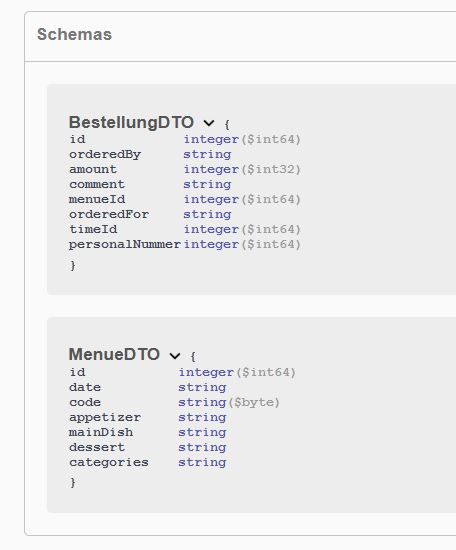
\includegraphics[scale=0.40]{pics/swagger-schema.jpg}
    \caption{SwaggerUI}
    \label{fig:impl:swagger-schema}
\end{figure}







\begin{spacing}{1}
\chapter{Implementierung}\label{chapter:implementation}
\end{spacing}
\section {Systemarchitektur}
\author{Benjamin Besic}

\begin{figure}[htp]
    \centering
    \author{David Ignjatovic}
    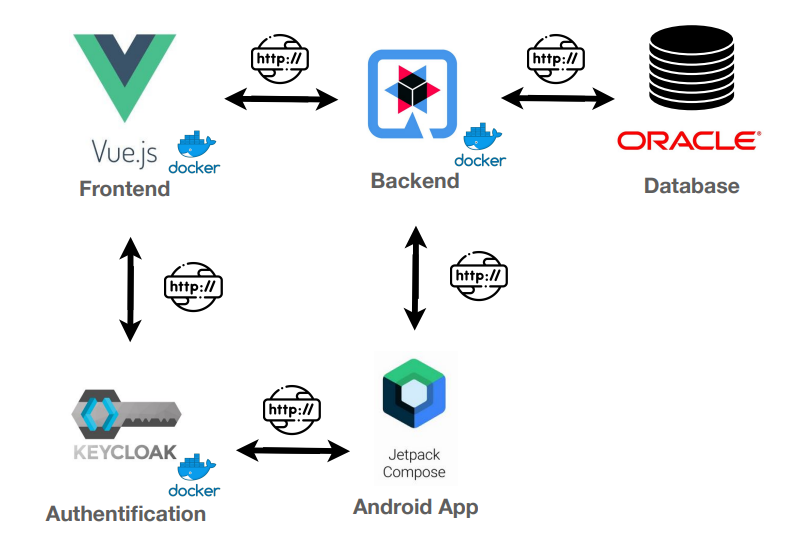
\includegraphics[scale=0.7]{pics/final-sys-arc.PNG}
    \caption{Systemarchitektur des Programms}
    \label{fig:impl:SysArc}
\end{figure}

Der Systemarchitektur kann man entnehmen, dass das Quarkus Backend die zentrale Stelle für alle anderen Technologien bildet.
Das Backend stellt mit Hilfe der Datenbank alle Daten zur Verfügung mittels REST. \\*
Der Keycloak Server sichert die beiden Frontends ab und sorgt dafür, dass keine ungewollten Zugriffe entstehen.
Vue.js benützt dafür ein Keycloak Package, dass eine leichte Integration erlaubt. Die Android App hingegen arbeitet mittels REST Requests mit Keycloak zusammen,
da es zum jetzigen Zeitpunkt keine offizielle Erweiterung für Jetpack Compose gibt.

\subsection{Technologien}

Beim Entwickeln wurden folgende Technologien verwendet:
\begin{itemize}
    \item docker 3.1
    \item Vue.js 2.6.14
    \item quarkus 2.5.0.Final
    \item Jetpack Compose 1.0.1
    \item Keycloak 14.0.0
    \item Java OpenJDK-11
    \item Java EE 8
    \item JBoss Wildfly 7.3.4.GA
\end{itemize}

\section{Datenmodell}
\author{David Ignjatovic}

Ein Datenmodell wird als Darstellung der relevanten Objekte eines Projektes verwendet. 
Unser Datenmodell ist im Großen und Ganzen immer gleichgeblieben. Für den Algorithmus aber haben wir es aber erweitern müssen.

\subsection{Use Cases}

\subsubsection{Kantinenarbeiter}

\begin{compactitem}
    \item Neue Menüs anlegen
    \begin{compactitem}
        \item Kantinenmitarbeitende können für jeden Tag neue Menüs mit drei Hauptspeisen und deren Kategorien, einer Vorspeise und einer Nachspeise anlegen.
    \end{compactitem}
    \item Vorhandene Menüs editieren
    \begin{compactitem}
        \item Die Bezeichnungen der bereits erstellten Menüs sollen verändert werden können.
    \end{compactitem}
    \item Übersicht der täglichen Bestellungen
    \begin{compactitem}
        \item Die Kantinenmitarbeitenden sollen eine Übersicht, der an einem bestimmten Tag bestellten Menüs haben. Diese inkludiert die zusammengefasste Bestellanzahl der verschiedenen Menüs und eine Liste von allen Bestellungen.
    \end{compactitem}
    \item Bestellungsübersicht drucken
    \begin{compactitem}
        \item Die Übersicht wie vorher beschrieben soll zu einem PDF-Objekt konvertiert werden und dementsprechend ausgedruckt werden können.
    \end{compactitem}
\end{compactitem}

\subsubsection{Mitarbeiter}

\begin{compactitem}
    \item Menüs bestellen
    \begin{compactitem}
        \item Ein Mitarbeiter hat eine Auswahl aller Menüs und kann für jeden Tag eine der drei Hauptspeisen auswählen. Nach der Auswahl kann er die Essenszeit auswählen, die Anzahl und nötige Kommentare hinzufügen.
    \end{compactitem}
    \item Menüs für andere Mitarbeiter bestellen
    \begin{compactitem}
        \item Ein Mitarbeiter kann den obrigen Bestellvorgang für einen anderen Mitarbeiter ausführen. 
    \end{compactitem}
    \item Übersicht aller Bestellungen
    \begin{compactitem}
        \item Als Mitarbeiter soll man alle seine vergangenen Bestellungen und deren Informationen in einer Übersicht einsehen können. Diese Übersicht kann filtriert werden.
    \end{compactitem}
    \item Bestellungen stornieren
    \begin{compactitem}
        \item In der oben genannten Übersicht soll man die Möglichkeit haben eine Bestellung auszuwählen und zu stornieren, wenn dies möglich ist.
    \end{compactitem}
    \item Bestellstatistiken einsehen
    \begin{compactitem}
        \item Ein Mitarbeiter soll Diagramme zur Verfügung haben, wo er sein Bestellverhalten einsehen kann.
    \end{compactitem}
\end{compactitem}

\subsection{Planung}
\author{Benjamin Besic}
Einer der ersten Arbeitsschritte war die Entwicklung eines Datenmodells, welches die Basis der Programmlogik sein soll. Dieses wurde mit einem ERD-Diagramm erstellt.
\begin{figure}[htp]
    \centering
    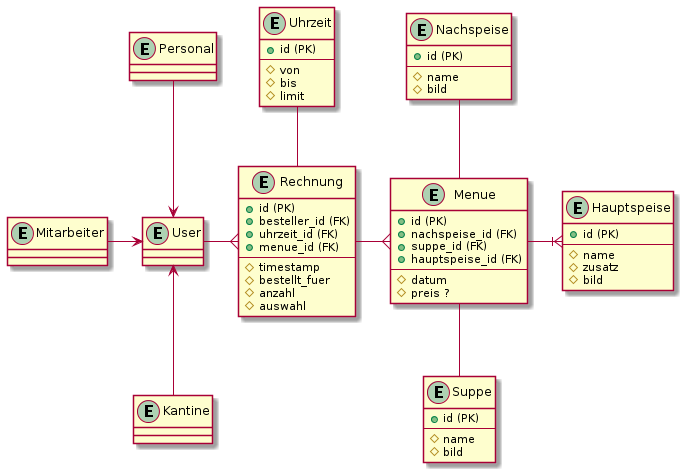
\includegraphics[scale=0.4]{pics/erd-alt.png}
    \caption{Erste Version des Datenmodells}
    \label{fig:impl:ERDold}
\end{figure}

Die erste Version wurde von unserem Team entwickelt, aus den Erfahrungen und Informationen, die wir im Unterricht gesammelt haben. \\*
An dieser Version merkt man, dass die meisten Teile in einzelne Tabellen aufgeteilt wurden. Dies sorgt für Flexibilität und Wiederverwendung von einem Menü, da die einzelnen
Speisen aufgeteilt sind.
Am Anfang war geplant, dass jede Speise auch ein Bild hat, damit der Mitarbeiter weiß, wie die Speise auch wirklich aussieht.\\*
Ebenfalls erkennt man, dass es eine User-Klasse gibt, da Mitarbeiter, Personal und Kantine gleiche Eigenschaften miteinander teilen wie zum Beispiel Vor- und Nachname.\\*


\begin{figure}[htp]
    \centering
    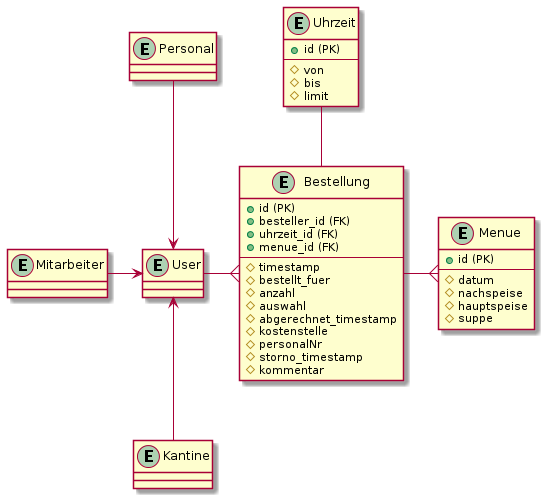
\includegraphics[scale=0.5]{pics/erd-aktuell.png}
    \caption{Finale Version des Datenmodells}
    \label{fig:impl:ERDnew}
\end{figure}

Die finale Version des Datenmodells übernimmt das meiste der ersten Version, jedoch wurde es nach Absprache mit unserer Partnerfirma überarbeitet, um deren Anforderungen mehr zu entsprechen.\\*
Eine wichtige Änderung ist, dass die Menue-Klasse alle Speisen enthält und diese als einfacher Text gespeichert werden. Der Grund dafür ist, dass die Kantine
immer die Menüs händisch eingibt und eine Auswahl von vorhandenen Speisen würde nur den Speicheraufwand unnötig erhöhen. Es kommt eher selten vor, dass die selben Speisen nacheinander kommen.\\*
Was vorher gefehlt hat war der Kommentar und die Möglichkeit die Stornierung eines Menüs nachzuvollziehen. Wenn ein Menü storniert wird, wird es nicht gelöscht, sondern es wird nur 
das Stornodatum gesetzt. Es ist wichtig, dass auch stornierte Bestellungen in der Datenbank bleiben. \\*
Ebenfalls wurde die Abrechnung eines Menüs in der ersten Version nicht berücksichtigt. Die Kosten für das Menü werden dem Mitarbeiter vom Gehalt abgezogen und dies erfolgt anhand 
von den Daten in der Datenbank.


\subsection{Entitäten}
\author{David Ignjatovic}

Eine Entität ist ein bestimmtes Objekt mit den jeweiligen Atributen. Atribute sind die Eigenschaften eins Objektes.
Unser Projektes beinhaltet 5 Entitäten:

\begin{itemize}
  \item Bestellung
  \item Categories
  \item Kantine
  \item Menue
  \item Oeffungszeit
\end{itemize}

\subsection{Bestellung} 

Die Entität \textbf{Bestellung} enthält die wichtigsten Informationen über einen Mitarbeiter und die dazu ausgewählte Mahlzeit.
Zur Identifikation einer Bestellung verwenden wir eine Id welche generiert wird. \\*

In der Bestellung wird angegeben von wem die Bestellung bestellt wurde und ob der Mitarbeiter es auch für sich selbst bestellt hat oder für jemand anderen. 
Jeder Mitarbeiter der Firma hat auch eine Personalnummer. Bei jeder Bestellung gibt es die Möglichkeit einen Kommentar abzugeben. Dieser wird an die Kantine mitgegeben. Natürlich hat man auch die Möglichkeit 
eine Mahlzeit öfters zu bestellen. Somit hat jeder Mitarbeiter die Möglichkeit eine Bestellanzahl mitzugeben. Für das Bestellen, Bearbeiten aber auch das Stornieren wird immer die jetzige Uhrzeit mitgegeben. \\*

Das wichtigste in der Bestellung ist die Mahlzeit und für wann es bestellt wurde. Dafür verwenden wir die zwei Klassen, Oeffnungszeit und Menue. \\*


\definecolor{dkgreen}{rgb}{0,0.6,0}
\definecolor{gray}{rgb}{0.5,0.5,0.5}
\definecolor{mauve}{rgb}{0.58,0,0.82}

\lstset{frame=tb,
  language=Java,
  aboveskip=3mm,
  belowskip=3mm,
  showstringspaces=false,
  columns=flexible,
  basicstyle={\small\ttfamily},
  numbers=none,
  numberstyle=\tiny\color{gray},
  keywordstyle=\color{blue},
  commentstyle=\color{dkgreen},
  stringstyle=\color{mauve},
  breaklines=true,
  breakatwhitespace=true,
  tabsize=3
}

\subsection{Categories}

Die Entität \textbf{Categories} ist ein Enum, welches wir hauptsächlich für unseren Algorithmus verwenden. Es besteht aus 4 Einträgen: \\*


\begin{itemize}
    \item Vegetarisch
    \item Vegan
    \item Schwein
    \item Rind
    \item Huhn
    \item Pute
    \item Salat
    \item Nudel
    \item Süß
    \item Fisch
    \item Sonstiges
\end{itemize}

Die einzelnen Kategorien beschreiben eine Mahlzeit. Sommit kann man ganz einfach zwischen einzelnen Mahlzeiten unterscheiden und sie auch gruppieren.


\subsection{Kantine}

In der Entitäten \textbf{Kantine} befinden sich die wichtigsten Informationen über eine Kantine wie zum Beispiel ob eine Kantine offen hat oder zurzeit geschlossen ist. 
Eine kleine Beschreibung über die Kantine und über das Service ist ebenso enthalten. \\*

\pagebreak

\subsection{Menue}

In der Entität \textbf{Menue} stehen die wichtigsten Informationen über ein Menü. Ein Menü beinhaltet eine Vorspeise, Hauptspeise, Nachspeise und ein Dessert. 
Noch dazu findet man in der Entität ein Datum, um zuzuordnen wann das Menü bestellt worden ist. \\*

Neben dem Bestelldatum beinhaltet die Entität Menue auch noch weitere Timestamps.
Die verwendeten Timestamps werden verwendet, um zu speichern, wann ein Menü erstellt wurde oder wann ein Menü geändert wurde. 
Natürlich wird auch mitgespeichert, von wem diese Änderungen durchgeführt worden sind. \\*


Die bereits oben genannten Kategorien finden wir in der Entität \textbf{Menue}. 
Diese werden verwendet, um einzelne Menüs zu unterscheiden und mit Hilfe der Kategorien und unserem Algorithmus kann man einfach hervorwagen welche Mahlzeit zu welchem Mitarbeiter am besten passt. \\*

Für jedes Menü wird auch die dazu ausgewählte Kantine mitgespeichert. So weiß man, zu welcher Kantine der Mitarbeiter gehen muss, um sein Menü zu bekommen. \\*



\subsection{Oeffnungszeit}

Die Entitäten \textbf{Oeffnungszeit} zeigt an, ob ein Kantinenraum in Verwendung ist und ob die maximale Anzahl an Sitzplätzen schon belegt ist. 
Das Zeitfenster, welches beschreibt wann gegessen wird, wird ebenso mitgespeichert. \\*

Um zu wissen, welcher Kantinenraum gemeint wird, wird auch die verwendete Kantine mitgespeichert. \\*

\pagebreak

\section{REST-Schnittstellen}

\colorlet{punct}{red!60!black}
\definecolor{background}{HTML}{EEEEEE}
\definecolor{delim}{RGB}{20,105,176}
\colorlet{numb}{magenta!60!black}

\lstdefinelanguage{json}{
    basicstyle=\normalfont\ttfamily,
    numbers=left,
    numberstyle=\scriptsize,
    stepnumber=1,
    numbersep=8pt,
    showstringspaces=false,
    breaklines=true,
    frame=lines,
    backgroundcolor=\color{background},
    literate=
     *{0}{{{\color{numb}0}}}{1}
      {1}{{{\color{numb}1}}}{1}
      {2}{{{\color{numb}2}}}{1}
      {3}{{{\color{numb}3}}}{1}
      {4}{{{\color{numb}4}}}{1}
      {5}{{{\color{numb}5}}}{1}
      {6}{{{\color{numb}6}}}{1}
      {7}{{{\color{numb}7}}}{1}
      {8}{{{\color{numb}8}}}{1}
      {9}{{{\color{numb}9}}}{1}
      {:}{{{\color{punct}{:}}}}{1}
      {,}{{{\color{punct}{,}}}}{1}
      {\{}{{{\color{delim}{\{}}}}{1}
      {\}}{{{\color{delim}{\}}}}}{1}
      {[}{{{\color{delim}{[}}}}{1}
      {]}{{{\color{delim}{]}}}}{1},
}

\subsection{Allgemein}

In den folgenden Beispielen läuft unser Server lokal auf dem Port 8080. Die URL über die unser
Server erreicht werden kann, lautet: \textbf{\textit{http://localhost:8080/menue}}.

\subsection{Bestellung}

\subsubsection{Bestellungen von einem Mitarbeiter}

Um zu sehen welche Bestellungen ein Mitarbeiter hat, muss der Pfad \textbf{\textit{/bestellung/<username>}} aufgerufen werden. 
Hierbei handelt es sich um eine GET-Methode die mittels Path Parameter die Bestellungen eines bestimmten Mitarbeiters zurück gibt.
Wenn ein Mitarbeiter gefunden wurde und dieser auch mindestens eine Bestellung hat wird der Status 200 zurückgegeben. \\*

Das Reslutat für den Mitarbeiter \textbf{spabo} sieht folgendermassen aus:


URL: GET \colorbox{white}{\lstinline[basicstyle=\ttfamily\color{black},language=html]| http://localhost:8080/menue/bestellung/spabo|}


Output:

\begin{lstlisting}[language=json,firstnumber=1]
{
    "createdAt": "2021-11-26T15:33:33.62898Z[UTC]",
    "id": 1315,
    "menueDate": "2021-11-29",
    "menueName": "Spaghetti",
    "orderedFor": "spabo",
    "timeWindow": "11:15 - 11:45"
}
\end{lstlisting}

Die Bestellungen wird nach dem Datum, an dem eine Bestellungen angelegt wurde, sortiert. Somit werden immer die neusten Bestellungen gleich am Anfgang angezeigt.

\pagebreak

\subsubsection{Anzahl der Bestellungen pro Wochentag eines Mitarbeitern}

Wenn man sehen will, wie oft ein Mitarbeiter pro Wochentag ein Menue bestellt hat, muss der Pfad \textbf{\textit{/bestellung/stats/<username>}} aufgerufen werden.
Es werden alle Wochentage angezeigt an denen ein Mitarbeiter eine Bestellung getätigt hat. Wenn mindestens ein Wochentag mit einer Bestellung zur verfügung steht, 
wird der Status 200 zurückgegeben.

Das Reslutat für den Mitarbeiter \textbf{besbe} sieht folgendermassen aus:


URL: GET \colorbox{white}{\lstinline[basicstyle=\ttfamily\color{black},language=html]|http://localhost:8080/menue/bestellung/stats/besbe|}


Output:

\begin{lstlisting}[language=json,firstnumber=1]
[
    {
    "amount": 2,
    "weekday": "Montag"
    },
    {
    "amount": 1,
    "weekday": "Mittwoch"
    },
    {
    "amount": 1,
    "weekday": "Donnerstag"
    },
    {
    "amount": 0,
    "weekday": "Dienstag"
    }
]
\end{lstlisting}

\pagebreak

\subsubsection{Alle Kategorien}

Damit man alle Kategorien sehen kann, die eine Mahlzeit beschreibt, muss der Pfad  \textbf{\textit{/bestellung/categories}} aufgerufen werden.
Wichtig ist es, dass man hier keinen Namen als Parameter übergibt. \\*

Anhand der Kategorien, wird mit Hilfe eines Algorithmus enschieden, welche Mahlzeit am besten zu einem Mitarbeiter passt. Es wird darauf geschaut, welche Kategorie
am häufigsten vorkommt.

Die verwendbaren Kategorien sehen folgendermassen aus:

URL: GET \colorbox{white}{\lstinline[basicstyle=\ttfamily\color{black},language=html]|http://localhost:8080/menue/bestellung/categories|}

Output:

\begin{lstlisting}[language=json,firstnumber=1]
[
    "Vegetarisch",
    "Vegan",
    "Schwein",
    "Rind",
    "Huhn",
    "Pute",
    "Salat",
    "Nudel"
    "Fisch",
    "Sonstiges"
]
\end{lstlisting}

Das wird hauptsächlich verwendet, um bei dem Frontend alle Kategorien anzuzeigen die für eine bestimmte Mahlezeit dazugehören.

\pagebreak

\subsubsection{Alle Kategorien von einem bestimmten Mitarbeiter}

Um zu sehen welche Kategorien ein Mitarbeiter bestellt hat, muss der Pfad \textbf{\textit{/bestellung/categories/<username>}} aufgerufen werden.

Wenn ein User keine Bestellungen getätigt hat, werden auch keine Kategorien zurückgegeben. In dem folgenden Beispiel kann man aber sehen, wie das Reslutat
für den Mitarbeiter \textbf{spabo} aussieht:

URL: GET \colorbox{white}{\lstinline[basicstyle=\ttfamily\color{black},language=html]|http://localhost:8080/menue/bestellung/categories/spabo|}

Output:

\begin{lstlisting}[language=json,firstnumber=1]
[
    "Vegetarisch",
    "Nudel",
    "Vegan",
    "Schwein",
    "Salat",
    "Pute"
]
\end{lstlisting}

\subsubsection{Alle Bestellungen an einem bestimmten Tag}

Damit die Kantine sehen kann, welche Bestellungen an welchen Tagen zugewissen worden sind, muss der Pfad \textbf{\textit{/bestellung?date=datum}} aufgerufen werden.

Es kann aber auch sein, das es an bestimmten Tagen keine Bestellungen gibt. Deshalb werden auch keine Ergebnisse zurückgegeben.

Um aber zu veranschaulichen, wie manche Bestellungen an einem bestimmten Zeitpunkt zurückgegeben werden, verwenden wir das den \textbf{16.03.2022}.

URL: GET \colorbox{white}{\lstinline[basicstyle=\ttfamily\color{black},language=html]|http://localhost:8080/menue/bestellung?date=2022-03-16|}

Output:

\begin{lstlisting}[language=json,firstnumber=1]
[
    {
        "code": "A",
        "date": "2022-03-16",
        "menue": "Schnitzel",
        "menueCounter": 1,
        "orderedFor": "spabo",
        "personalNumber": 1023,
        "timewindow": "11:15 - 11:45"
    },
    {
        "code": "C",
        "date": "2022-03-16",
        "menue": "Eisbergsalat",
        "menueCounter": 1,
        "orderedFor": "spabo",
        "personalNumber": 1023,
        "timewindow": "12:00 - 12:30"
    },
    ...
    ]
\end{lstlisting}


\subsubsection{Bestellung erstellen}

Wenn ein User eine Bestellung aufgeben will, muss der Pfad \textbf{\textit{/menue/bestellung}} aufgerufen werden. 
Mithilfe der id, die man von dem vorherigen Request bekommen hat, kann man ganz einfach seine Bestellung abgeben. \\*

Ein Beispiel für eine Bestellung sieht folgendermassen aus:

\begin{lstlisting}[language=json,firstnumber=1]
    {
        "orderedBy":"spabo",
        "amount":"1",
        "comment":"",
        "menueId":707,
        "orderedFor":"spabo",
        "timeId":6,
        "personalNummer":1023
    }
\end{lstlisting}

Wenn die Betellung erfolgreich war, wird der Status 200 zurückgegeben.


\subsubsection{Bestellung stornieren}

Um eine Betellung zu stornieren, muss der Pfad \textbf{\textit{/menue/bestellung}} aufgerufen werden. Wie auch bei dem Erstellen einer Bestellung wird 
mit Hilfe einer id die Bestellung zugeordnet. \\*

In unserer Datenbank wird die Bestellung nicht direkt gelöscht sondern überschrieben. Sie wird also auf gelöscht gesetzt, jedoch nicht aus der Datenbank gelöscht.

Wenn die Bestellung erfolgreich storniert wurde, wird die Antwort \textit{Order with id <is> was cancelled!} zurückgegeben.

\subsection{Menue}

\subsubsection{Alle Menüs}

Um sehen zu können, welche Menüs es überhapt schon gab, muss der Pfad \textbf{\textit{/menues}} aufgerufen werden. 

Ein Beispiel für ein Menue sieht folgendermassen aus:

URL: GET \colorbox{white}{\lstinline[basicstyle=\ttfamily\color{black},language=html]|http://localhost:8080/menue/menues|}


\begin{lstlisting}[language=json,firstnumber=1]
[
    {
        "appetizer": "Suppe",
        "categories": "Vegan;Vegetarisch;Salat",
        "code": "C",
        "date": "2022-03-22",
        "dessert": "Milka",
        "id": 706,
        "mainDish": "Kartofell Salat"
    },
    {
        "appetizer": "Suppe",
        "categories": "Vegan;Vegetarisch;Salat",
        "code": "C",
        "date": "2022-03-22",
        "dessert": "Milka",
        "id": 705,
        "mainDish": "Kartofell Salat"
    },
    ...
]
\end{lstlisting}

\subsubsection{Menü erstellen}

Damit die Kantine ein Menü erstellen kann, wird ein POST-Request an den Pfad \textbf{\textit{/menue/menues}} geschickt.

Da eine Bestellung aus genau 3 Menues besteht, werden auch 3 POST-Requests abgeschickt. Die werte werden in Form eines JSON Objekt abgeschickt.

Ein Beispiel für eine Bestellung sieht folgendermassen aus:

URL: POST \colorbox{white}{\lstinline[basicstyle=\ttfamily\color{black},language=html]|http://localhost:8080/menue/menues/|}


JSON Objekt für Menue A:

\begin{lstlisting}[language=json,firstnumber=1]
{
    "id":null,
    "date":"2022-03-22",
    "code":"A",
    "appetizer":"Suppe",
    "mainDish":"Pasta",
    "dessert":"Milka",
    "categories":"Rind;Nudel"
}
\end{lstlisting}

JSON Objekt für Menue B:

\begin{lstlisting}[language=json,firstnumber=1]
{
    "id":null,
    "date":"2022-03-22",
    "code":"B",
    "appetizer":"Suppe",
    "mainDish":"Lachs",
    "dessert":"Milka",
    "categories":"Fisch"
}
\end{lstlisting}

JSON Objekt für Menue C:

\begin{lstlisting}[language=json,firstnumber=1]
{
    "id":null,
    "date":"2022-03-22",
    "code":"C",
    "appetizer":"Suppe",
    "mainDish":"Kartofell Salat",
    "dessert":"Milka",
    "categories":"Vegan;Vegetarisch;Salat"
}
\end{lstlisting}

Wie man sehen kann, werden die Kategorien in einem String übergeben. Die Kategorien werden dann getrennt und als Enum gespeichert.

\subsubsection{Menü verändern}

Wie auch bei dem Erstellen eines Menüs, wird der Pfad \textbf{\textit{/menue/menues}} aufgerufen. 

Wie schon erwähnt, besteht eine Bestellung aus genau 3 Menüs, deswegen werden auch 3 PUT-Requests abgeschickt.

Ein Beispiel für eine Bestellung sieht folgendermassen aus:

URL: PUT \colorbox{white}{\lstinline[basicstyle=\ttfamily\color{black},language=html]|http://localhost:8080/menue/menues/|}

JSON Objekt für Menue A:

\begin{lstlisting}[language=json,firstnumber=1]
{
    "id":null,
    "date":"2022-03-22",
    "code":"A",
    "appetizer":"Suppe",
    "mainDish":"Pasta",
    "dessert":"Milka",
    "categories":"Rind;Nudel"
}
\end{lstlisting}

JSON Objekt für Menue B:

\begin{lstlisting}[language=json,firstnumber=1]
{
    "id":null,
    "date":"2022-03-22",
    "code":"B",
    "appetizer":"Suppe",
    "mainDish":"Lachs",
    "dessert":"Milka",
    "categories":"Fisch"
}
\end{lstlisting}

JSON Objekt für Menue C:

\begin{lstlisting}[language=json,firstnumber=1]
{
    "id":null,
    "date":"2022-03-22",
    "code":"C",
    "appetizer":"Suppe",
    "mainDish":"Kartofell Salat",
    "dessert":"Milka",
    "categories":"Vegan;Vegetarisch;Salat"
}
\end{lstlisting}

\subsubsection{Menü-Vorschlag (Recommendation)}

Wenn ein Mitarbeiter nicht weiß, welche Mahlezeit er wählen soll, wird mithilfe eines Recommender entschieden, welche Mahlzeit am besten dem 
User passt.  

Um die passende Mahlezeit zu bekommen, muss der Pfad \textbf{\textit{/menue/menues/recommendation}} aufgerufen werden.

Der Algorithmus sieht folgendermassen aus:

URL: PUT \colorbox{white}{\lstinline[basicstyle=\ttfamily\color{black},language=html]|http://localhost:8080/menue/menues/recommendation|}

\begin{lstlisting}
    public Menue  getRecommendation(String name, String date){
        List<String> categories = bestellungRepository.getALlCategoriesByUsername(name);
        List<Menue> menues = getMenuesByDate(date);
        Menue recommendedMenue = null;

        for (String category : categories){
            if(recommendedMenue != null){
                break;
            }
            for (Menue m : menues){
                if(recommendedMenue != null){
                    break;
                }

                String[] categorieOfMenue = m.getCategories().split(";");

                for (String c : categorieOfMenue){
                    if (category.equals(c)){
                        recommendedMenue = m ;
                        break;
                    }
                }
            }
        }
        return recommendedMenue;
    }
\end{lstlisting}

Um herausfinden zu können welche Mahlzeit optimal wäre, werden mit Hilfe des Algorithmus alle Kategorien des Users aus der Datenbank gehollt. 
Jeder User der eine Bestellung getätigt hat, hatte die höglichkeit zu sehen, welche Kategorien die Mahlzeit auch besitzt. Sommit kann man leicht herauszufinden
welche Kategorien auch am häufigsten in der Bestellhistorie vorkommen. \\*

Unser Algorithmus würde nicht funktionieren, gäbe es keine Bestellungen oder Mahlzeiten würden keine Kategorien besitzten. 
In anderen Worten, desto mehr Bestellungen man hat, umso genauer wird die recommendation. \\*

Die Kategorien werden in der Datenbank als string gespeichert die mit einem Strichpunkt geteilt werden. Hat man also bei einer Mahlzeit mehr als eine Kategorie,
so wird dieser als string mit einem oder mehreren Strichpunkten gespeichert. \\*

Hier ein paar Beispiele:

\textit{Schnitzel mit Pommes} = \textbf{"Schwein"}

\textit{Eisbergsalat} = \textbf{"Vegan;Vegetarisch"}

\textit{Nudelsalat mit Hühnerfleisch} = \textbf{"Nudel;Salat;Huhn"}

\subsubsection{Alle Menüs an einem bestimmten Tag}

Um alle Menüs an einem bestimmten Tag zu bekommen, wird der Pfad \textbf{\textit{/menue/menues/<date>}} aufgerufen.

Ein Beispiel für paar Menüs, welche am 12.08.2021 bestellt worden sind, sieht folgendermassen aus:

URL: PUT \colorbox{white}{\lstinline[basicstyle=\ttfamily\color{black},language=html]|http://localhost:8080/menue/menues/2021-12-08|}


\begin{lstlisting}[language=json,firstnumber=1]
{
    [
        {
            "appetizer": "Nudelsuppe",
            "categories": "Schwein",
            "changedAt": "2021-12-07T19:29:08.840936Z[UTC]",
            "changedBy": "IF170009:IF170009:beni",
            "code": "A",
            "createdAt": "2021-12-07T18:37:30.322514Z[UTC]",
            "createdBy": "IF170009:beni",
            "date": "2021-12-08",
            "desert": "Obst",
            "id": 499,
            "kantine": {
            "canteenDesc": "Betriebskueche",
            "changedAt": "2021-11-25T21:29:47.471379Z[UTC]",
            "changedBy": "IF170009:beni",
            "createdAt": "2021-11-25T21:29:47.471196Z[UTC]",
            "createdBy": "IF170009:beni",
            "id": 3,
            "serviceDesc": "Mittagstisch - CORONA LIGHT",
            "status": "A"
            },
            "mainDish": "Schweineschnitzel"
        },
        {
            "appetizer": "Nudelsuppe",
            "categories": "Rind;Nudel",
            "changedAt": "2021-12-07T19:29:08.995487Z[UTC]",
            "changedBy": "IF170009:IF170009:beni",
            "code": "B",
            "createdAt": "2021-12-07T18:37:30.490055Z[UTC]",
            "createdBy": "IF170009:beni",
            "date": "2021-12-08",
            "desert": "Obst",
            "id": 500,
            "kantine": {
            "canteenDesc": "Betriebskueche",
            "changedAt": "2021-11-25T21:29:47.471379Z[UTC]",
            "changedBy": "IF170009:beni",
            "createdAt": "2021-11-25T21:29:47.471196Z[UTC]",
            "createdBy": "IF170009:beni",
            "id": 3,
            "serviceDesc": "Mittagstisch - CORONA LIGHT",
            "status": "A"
            },
            "mainDish": "Lasagne"
        },
        ...
    ]
}
\end{lstlisting}

Hier sieht man die wichtigsten Daten wie zum Beispiel die Vorspeise, Hauptspeise, Nachspeise und Desert welche von dem jeweiligem Mitarbeiter bestellt worden sind. 
Auch Daten wie die Bestellzeit und in welcher Kantine gegessen wird wird auch mitgegeben.

\subsubsection{Alle aktiven Essenszeiten}

Um zu sehen ob noch freie Sitzplätze zur Verfügung stehen, wird der Pfad \textbf{\textit{/menue/oeffnungszeiten}} aufgerufen. 

In unserer Kantine gibt es 4 Zeiten an denen man essen gehen kann. Diese dauern immer eine halbe Stunde und haben eine Zwischenpause von 15 min. 
Pro Essenszeit können maximal 20 Personen in dem Saal essen.

Ein Beispiel für die Öffnungszeiten und für die freien Plätze sieht folgendermassen aus:

URL: PUT \colorbox{white}{\lstinline[basicstyle=\ttfamily\color{black},language=html]|http://localhost:8080/menue/menues/2021-12-08|}


\begin{lstlisting}[language=json,firstnumber=1]
{
    [
        {
            "chosen": false,
            "freeSeats": -1,
            "id": 6,
            "maxSeats": 20,
            "time": "11:15 - 11:45"
        },
        {
            "chosen": false,
            "freeSeats": -1,
            "id": 7,
            "maxSeats": 20,
            "time": "12:00 - 12:30"
        },
        {
            "chosen": false,
            "freeSeats": -1,
            "id": 8,
            "maxSeats": 20,
            "time": "12:45 - 13:15"
        },
        {
            "chosen": false,
            "freeSeats": -1,
            "id": 9,
            "maxSeats": 20,
            "time": "13:30 - 14:00"
        }
    ]
}
\end{lstlisting}

\section{Authentifizierung}

\section {Interface Webapp}
\author{Benjamin Besic}
\subsection{Planung}

Nachdem das Datenmodell feststand wurden UI-Prototypen entwickelt, die das Aussehen der Vue-App darstellen sollen.

\begin{figure}[htp]
    \author{Benjamin Besic}
    \centering
    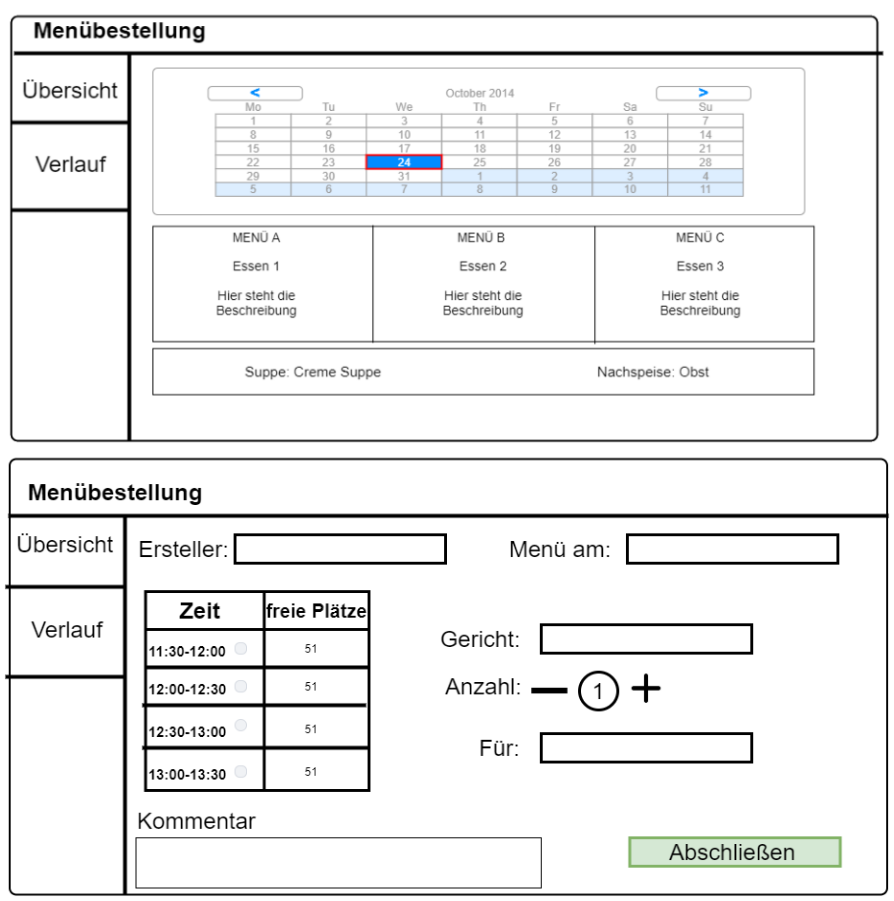
\includegraphics[scale=0.3]{pics/UI-Bestellung-Prototyp.png}
    \caption{UI-Prototypen für den Bestellvorgang}
    \label{fig:impl:UIPlanningBest}
\end{figure}

\subsubsection{Bestellvorgang}
Beim Entwickeln stehen die Benutzerfreundlichkeit und das Aussehen auf mobilen Geräten an erster Stelle. Anhand dessen ist die Navigationsleiste am Wichtigsten.
Diese soll den Benutzer auf alle Sichten führen können und dem Benutzer ermöglichen, sich auszuloggen. \\*
Der Kalender muss übersichtlich sein und die Tage, an denen Bestellungen nicht möglich sind, sollten ausgeblendet sein. Ebenfalls soll auch in die Vergangenheit geschaut werden können.\\*
Um den Rest des Platzes auszunutzen wurde eine Menüauswahlt geplant, die soviel wie möglich Information darstellen kann, ohne den Benutzer zu überfordern.
Nach langem Überlegen wurden die drei Menüs groß als Kästen dargestellt, um soviel wie möglich innerhalb dieser darstellen zu können.
Die Vor- und Nachspeise ist kleiner dargestellt, da man keine Entscheidung darüber machen kann.\\*
Die Sicht nachdem man sich ein Menü ausgewählt hat, soll so kompakt wie möglich sein, da auch die mobile Ansicht ohne Probleme nutzbar sein soll.
Alle Informationen, die vom Benutzer eingegeben werden müssen, sollen in der Form eines Formulars angezeigt werden und andere Informationen wie Ersteller und Gericht 
werden automatisch eingesetzt.
\begin{figure}[htp]
    \author{Benjamin Besic}
    \centering
    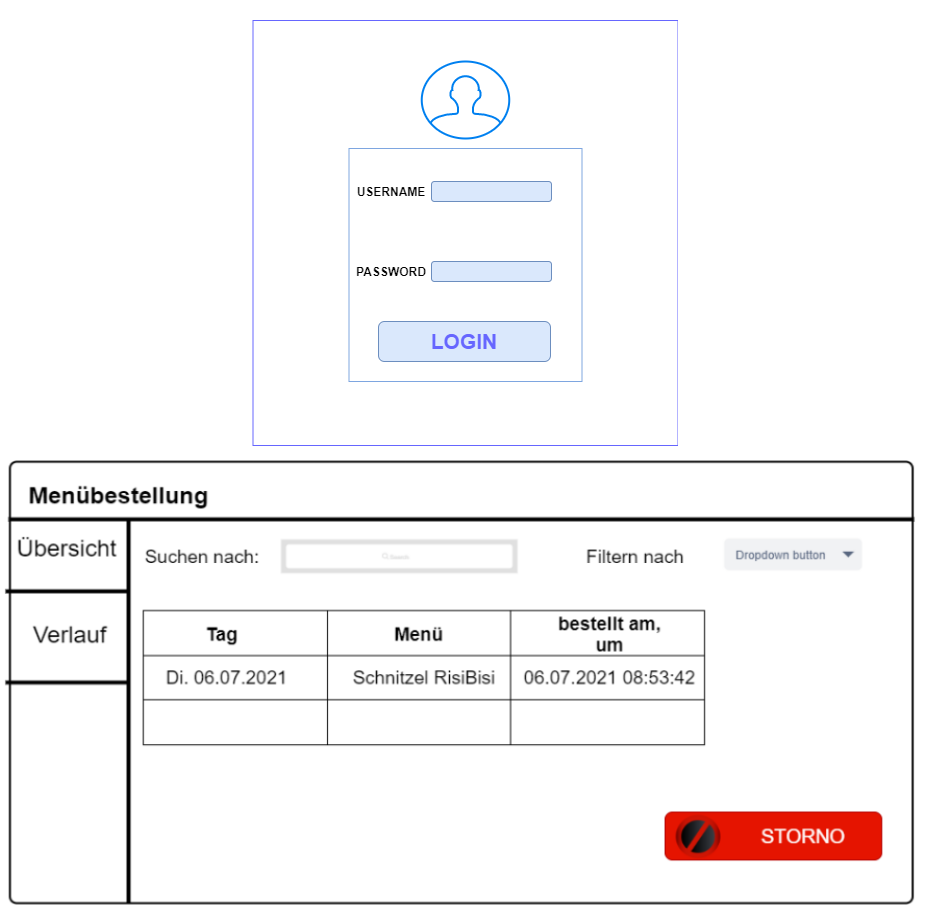
\includegraphics[scale=0.36]{pics/UI-Login-Uebersicht-Prototyp.png}
    \caption{UI-Prototypen für den den Login und die Übersicht}
    \label{fig:impl:UIPlanningLogUebersicht}
\end{figure}

\subsubsection{Login und Übersicht}
Der Login soll einladend sein, hat aber keinen besonderen Anforderungen zu entsprechen \\*
Die Übersicht über die bereits bestellten Menüs soll dem Benutzer alle wichtigen Informationen auf einen Blick geben.
Das Stornieren soll ebenfalls simpel gehalten werden, damit der Benutzer nicht darüber nachdenken muss.
Der Benutzer soll auch eine Möglichkeit haben die Bestellungen zu filtern, um bestimmte Zeitpunkte bzw. Menüs einfacher zu finden.


\subsection{Login}
Beim Aufrufen der Webapp wird man zunächst zu der Login-Seite weitergeleitet. Wie diese fungiert, sieht man in der nächsten Abbildung. \\*
Der Login dient in erster Hinsicht dazu, um festzustellen ob der Benutzer ein Mitarbeiter oder Kantinenmitarbeiter ist.
Denn nach dem Login wird man entweder zur Mitarbeiter-Ansicht oder Kantinenmitarbeiter-Ansicht weitergeleitet. \\*

\begin{figure}[htp]
    \centering
    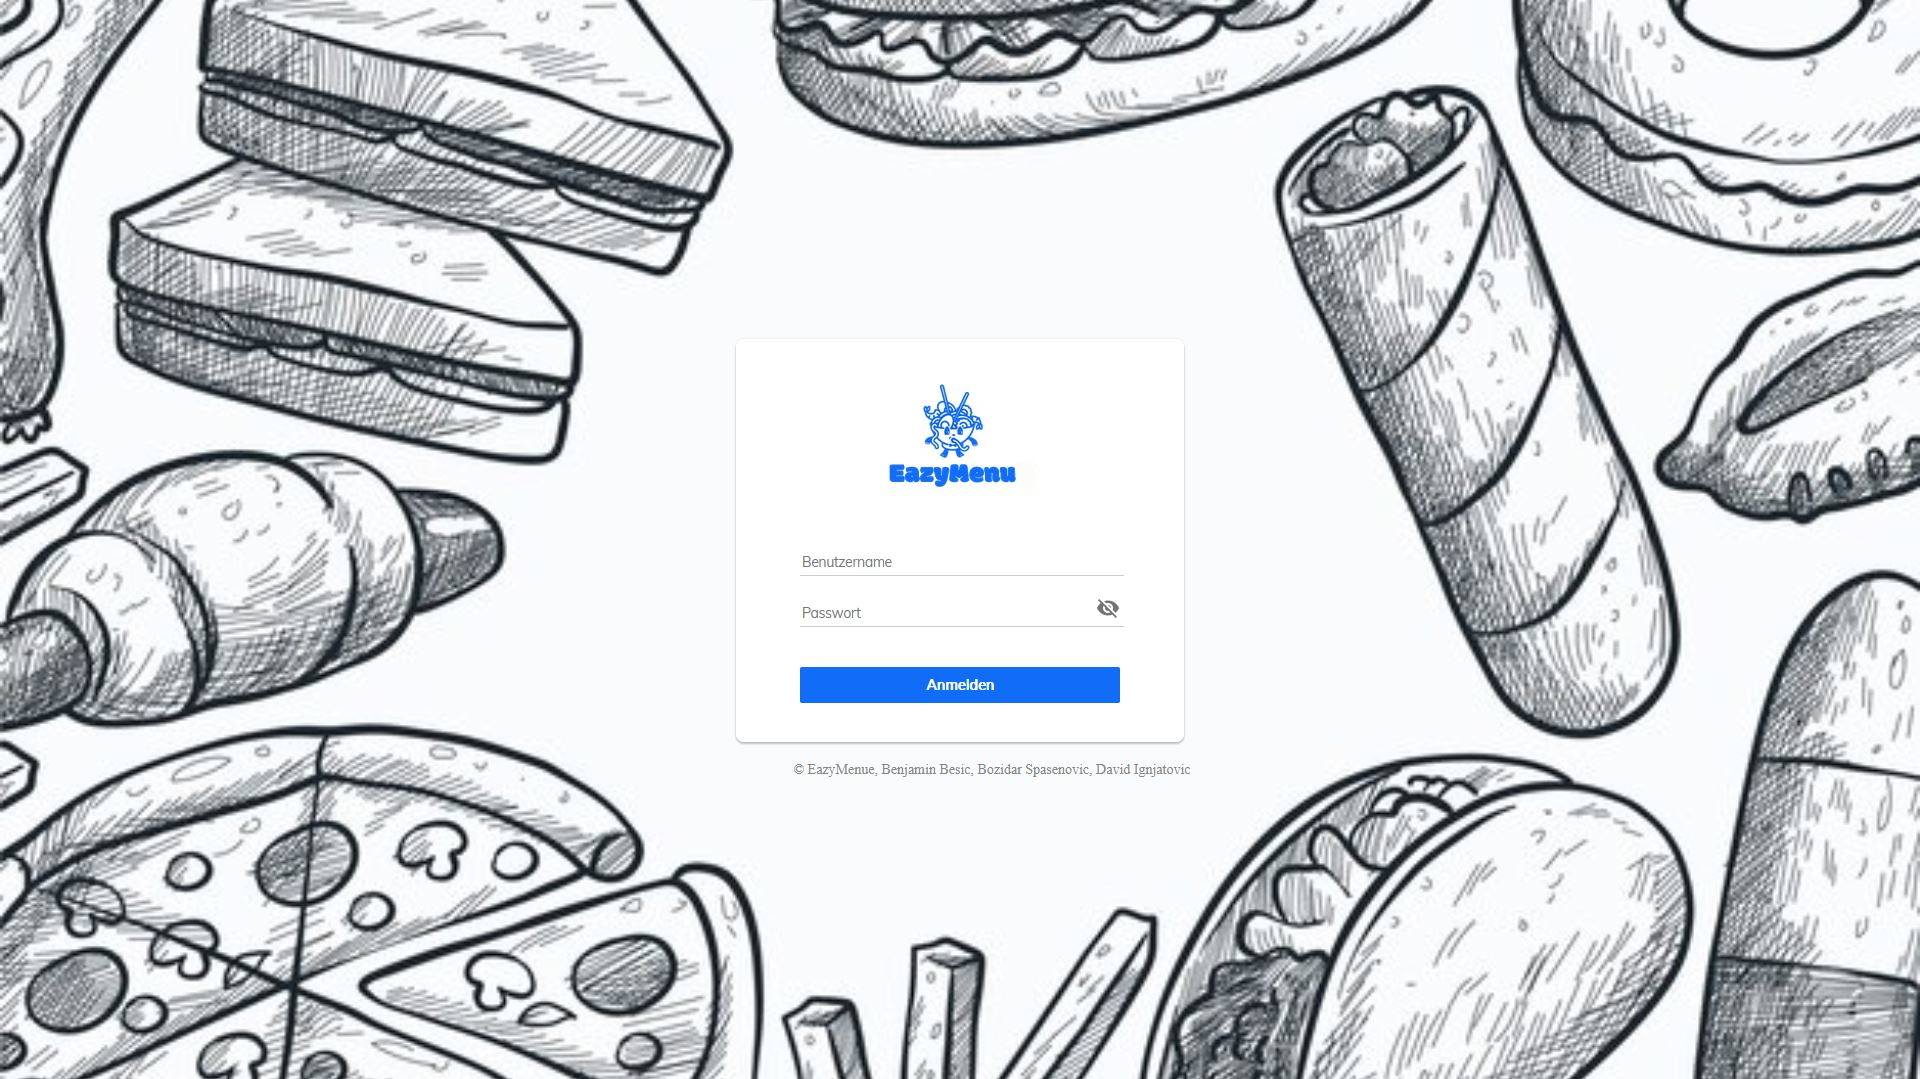
\includegraphics[scale=0.3]{pics/login_screen_vue.JPG}
    \caption{Login Screen}
    \label{fig:impl:LoginVue}
\end{figure}


\pagebreak

\subsection {Mitarbeiter-Ansicht}

\subsubsection {Home}
\label{sec:MitHome}
Das Erste, was ein Mitarbeiter zu sehen bekommt, ist die Home Ansicht. In dieser Ansicht ist eine Kalender und die Menüauswahl enthalten. \\*
Der Benutzer kann im Kalender das gewünschte Bestelldatum anklicken, dadurch wird automatisch die Menüauswahl aktualisiert. Man kann sich in die Zukunft, sowohl auch 
in die Vergangenheit klicken, um sich Auskunft über die vergangenen/kommenden Menüs zu beschaffen. Die Ansicht ist nur auf die Bestelltage beschränkt, an denen Menüs angeboten werden.\\*
Nach der erfolgreichen Datumswahl hat man unten drei Menüs zur Auswahl, sowohl wie die dazugehörige Vor- und Nachspeise. Das dem Benutzer empfohlene Menü (Analyse aus seinem Bestellverlauf) wird grün hinterlegt.
Neben den Bestellköpfen befindet sich ein Fragezeichen-Knopf, wenn man über diesen geht werden einem die Kategorien des Menüs angezeigt.
\\* Wenn die Bedingungen für eine Bestellung erfüllt sind,
kann man auf einen der drei Bestellknöpfe drücken, um zur Bestellansicht weitergeleitet zu werden. Sind diese Bedingungen nicht erfüllt, sind die Knöpfe ausgeschaltet. \\*
Weiters werden unter den Menüs noch relevante Informationen angezeigt. Durch das Klicken des Fragezeichen-Knopfs wird ein Bild der 14 Allergene geöffnet.

\begin{figure}[htp]
    \centering
    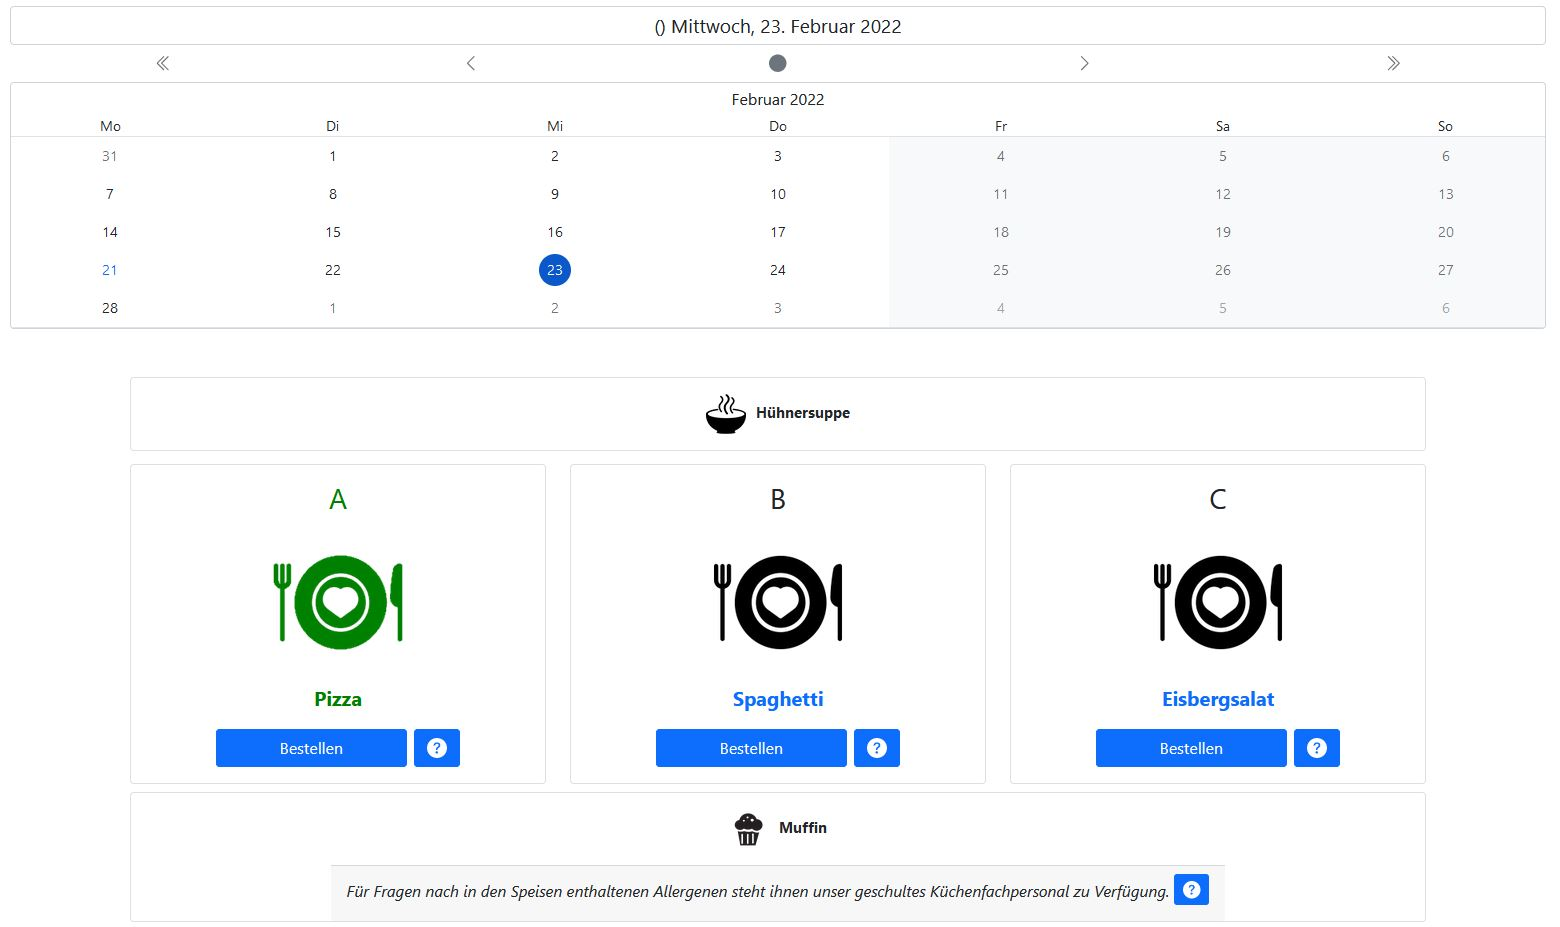
\includegraphics[scale=0.35]{pics/mitarbeiter-home.JPG}
    \caption{Home Ansicht eines Mitarbeiters}
    \label{fig:impl:HomeMitarbeiter}
\end{figure}

\begin{figure}[htp]
    \centering
    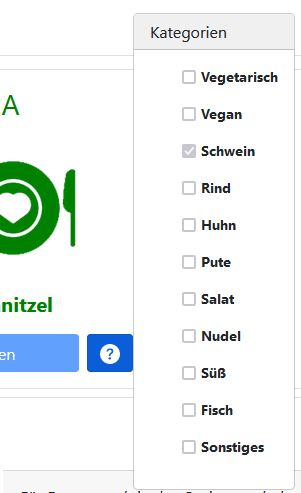
\includegraphics[scale=0.5]{pics/kategorien_mitarbeiter.JPG}
    \caption{Kategorieanzeige eines Menüs}
    \label{fig:impl:CategoriesForMenue}
\end{figure}

\pagebreak

\subsubsection {Bestellansicht}

In der Bestellansicht werden die nötigen Daten für die Bestellung ausgefüllt. Die ersten drei Felder sind automatisch ausgefüllt, aufgrund der vorherigen Auswahl. \\*
Die Tabelle auf der rechten Seite enthält alle Bestellzeiträume, die es gibt. Man kann nur eine gleichzeitig auswählen. Außerdem stehen die freien Plätze dabei, die aus der Datenbank geladen werden.\\*
Die Anzahl der Menüs kann durchs Klicken des Plus- und Minusknopfs angepasst werden.  \\*
Darunter steht voreingestellt der Benutzer, doch dies kann verändert werden, um das Menü für einen anderen Mitarbeiter bestellen zu können. \\*
Abschließend kann man noch einen Kommentar an die Kantine mitgeben, falls es etwaige Extrawünsche geben sollte. \\*
Die Bestellung kann durch den Abschließen-Knopf durchgeführt werden und Abbrechen kann man jederzeit mit dem Abbrechen-Knopf.
Die Bestellung ist erst ausführbar, sobald alle Felder außer des Kommentars ausgefüllt wurden.
\begin{figure}[htp]
    \centering
    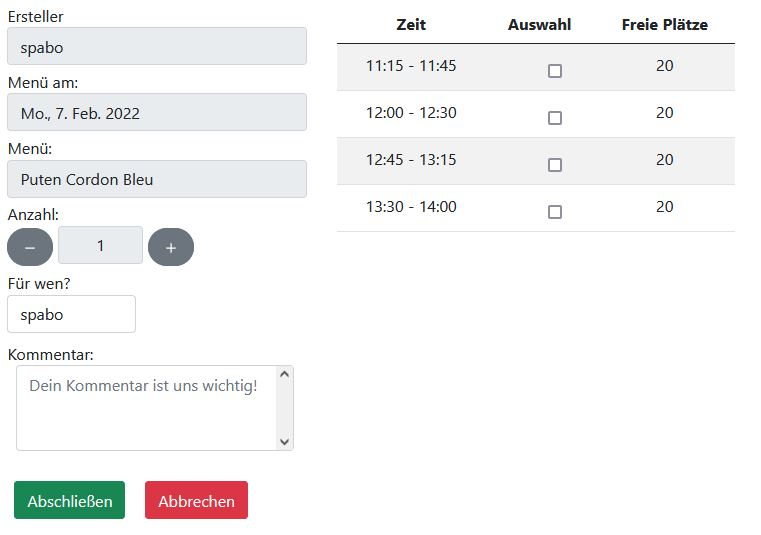
\includegraphics[scale=0.7]{pics/mitarbeiter-bestellen.JPG}
    \caption{Bestellansicht}
    \label{fig:impl:BestellenMitarbeiter}
\end{figure}
\pagebreak

\subsubsection {Bestellübersicht}

Die Bestellübersicht dient dem Benutzer dazu seine Bestellhistorie nachzuvollziehen. Zu jeder Bestellung ist der Name des bestellten Menüs, das Menüdatum, der Bestellzeitpunkt und die Essenszeit zugeordnet. \\*
Der Benutzer hat die Möglichkeit, oben in der Suchleiste, die Bestellungen nach Name oder Menüdatum zu filtern. Das Filtern erfolgt direkt nach der Eingabe. \\*
Man kann jede Bestellung anklicken und falls eine Bestellung die Stornierbedingungen erfüllt kann diese mit dem unten gelegen Storno-Button storniert werden.
Nach einer erfolgreichen Stornierung verschwindet die Bestellung aus dem Verlauf, doch in der Datenbank wird nur das Stornierdatum gesetzt und somit wird die Bestellung ungültig gemacht. 


\begin{figure}[htp]
    \centering
    \includegraphics[scale=0.3]{pics/mitarbeiter-bestellen-übersicht.JPG}
    \caption{Bestellungsübersicht}
    \label{fig:impl:BestellenMitarbeiterUebersicht}
\end{figure}
\pagebreak

\subsubsection {Statistiken}

Der Benutzer kann in dieser Ansicht mehr Informationen über seine vergangenen Bestellungen bekommen.
Durch das Wechseln des Tabs oben links wird entweder eine Statistik über die Kategorien oder über die Wochentage angezeigt. \\*
Die Informationen der Statistiken beziehen sich auf alle Bestellungen, die der Nutzer bereits getätigt hat.

\begin{figure}[htp]
    \centering
    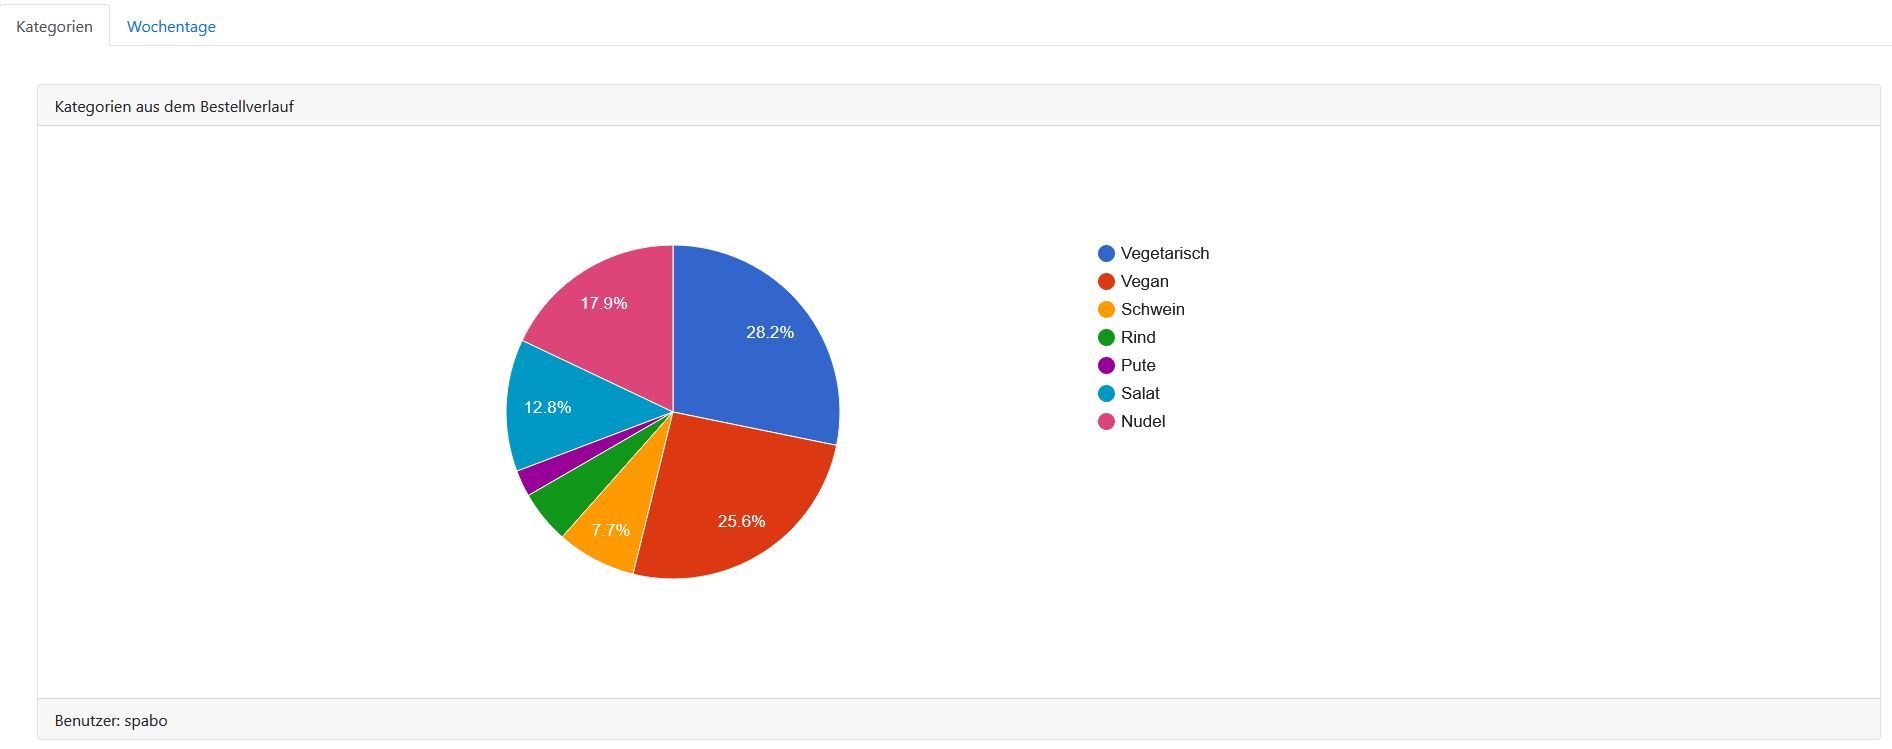
\includegraphics[scale=0.3]{pics/statistiken_kategorien.JPG}
    \caption{Kategorie Statistiken}
    \label{fig:impl:StatsCategories}
\end{figure}

\begin{figure}[htp]
    \centering
    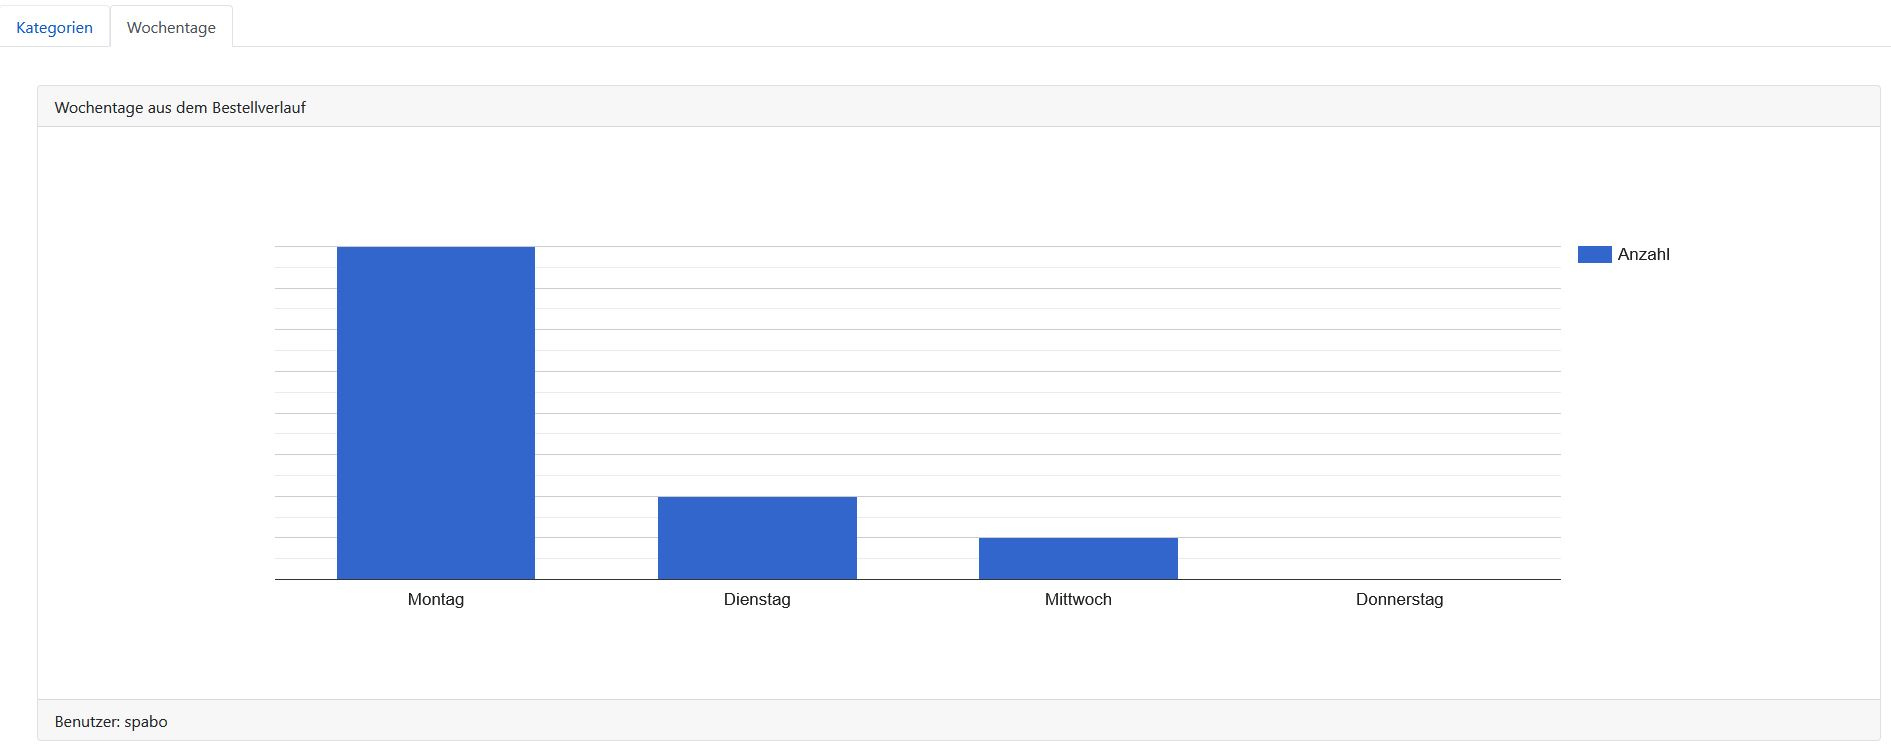
\includegraphics[scale=0.3]{pics/statistiken_wochentage.JPG}
    \caption{Wochentage Statistiken}
    \label{fig:impl:WeekDaysCategories}
\end{figure}

\pagebreak

\subsection {Kantinen-Ansicht}
\subsubsection {Home}

Die Startseite der Kantinenmitarbeiter ähnelt der Ansicht der Mitarbeiter. \hyperref[sec:MitHome]{Siehe hier}. \\*
Die Unterschiede sind, dass die Kantine Textfelder für jedes Menü und dessen Vor- und Nachspeise hat.
Ebenfalls erscheint beim Kategorien-Knopf eine Liste von Kategorien zum Anhaken, um dem Menü die entsprechenden Kategorien zuzuordnen. \\*
Die Textfelder und Kategorien können bearbeitet werden, um ein vorhandenes Menü zu aktualisieren oder um ein neues zu erstellen.
Die Erstellung bzw. die Änderung kann durch den Speichern-Knopf durchgeführt werden. Je nach Fall werden neue Menüs an das Backend geschickt oder ein
vorhandenes wird aktualisiert.

\begin{figure}[htp]
    \centering
    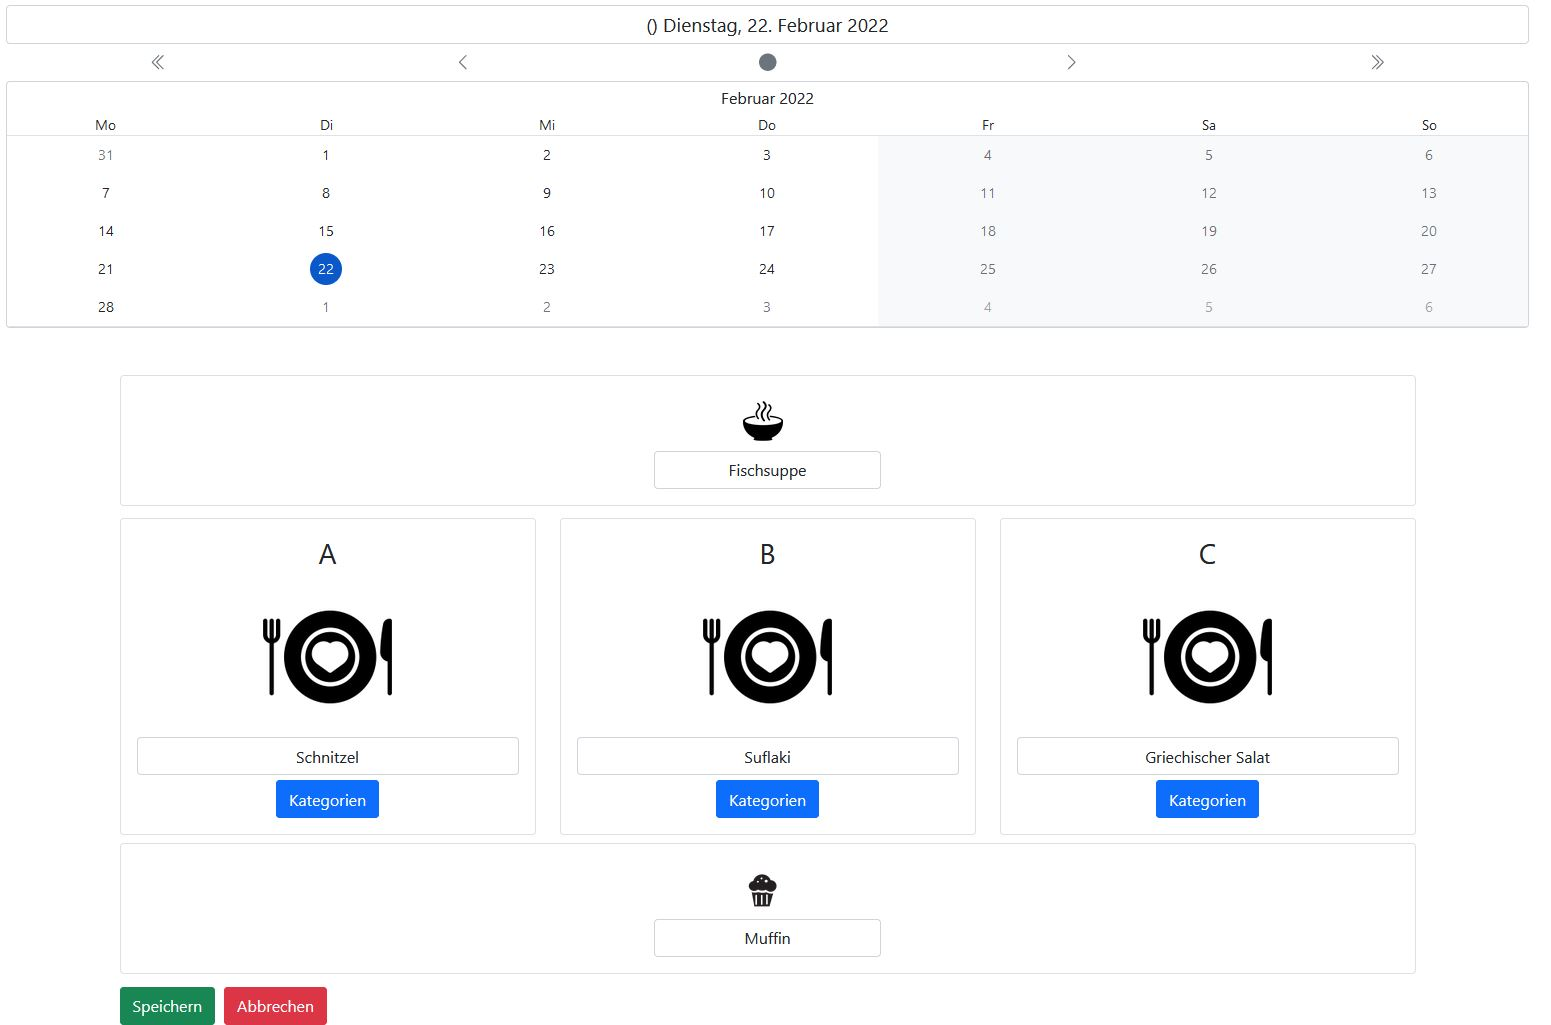
\includegraphics[scale=0.35]{pics/kantine_home.JPG}
    \caption{Kantine Homeansicht}
    \label{fig:impl:CantineHome}
\end{figure}

\begin{figure}[htp]
    \centering
    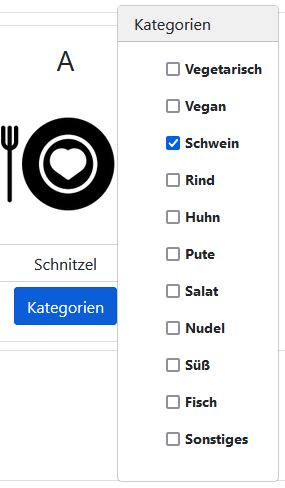
\includegraphics[scale=0.4]{pics/kategorien_kantine.JPG}
    \caption{Kategorieauswahl}
    \label{fig:impl:CategoryChooseCantine}
\end{figure}
\pagebreak

\subsubsection {Drucken}

Die Druckansicht dient den Kantinenmitarbeitern dazu, um die Bestellungen des jeweiligen Tages auch durchführen zu können.
Der Tag kann durch eine Datumsauswahl bestimmt werden.
Die Ansicht zeigt alle nötigen Informationen, damit die Kantine einen Überblick über die Bestellungen hat und dementsprechend das Essen vorbereiten kann.
Es sind die Essenszeiten sowie Anzahl der jeweiligen Menücodes summiert für einen schnellen Überblick. \\*
Durch das Drücken des Drucken-Knopfs hat die Kantine die Möglichkeit ein pdf-Dokument aus der kompletten Ansicht, die unter dem Knopf zu sehen ist, zu drucken.
Dies dient dazu, dass sie einen Ausdruck auf Papier haben, der für die Kantine praktischer ist.

\begin{figure}[htp]
    \centering
    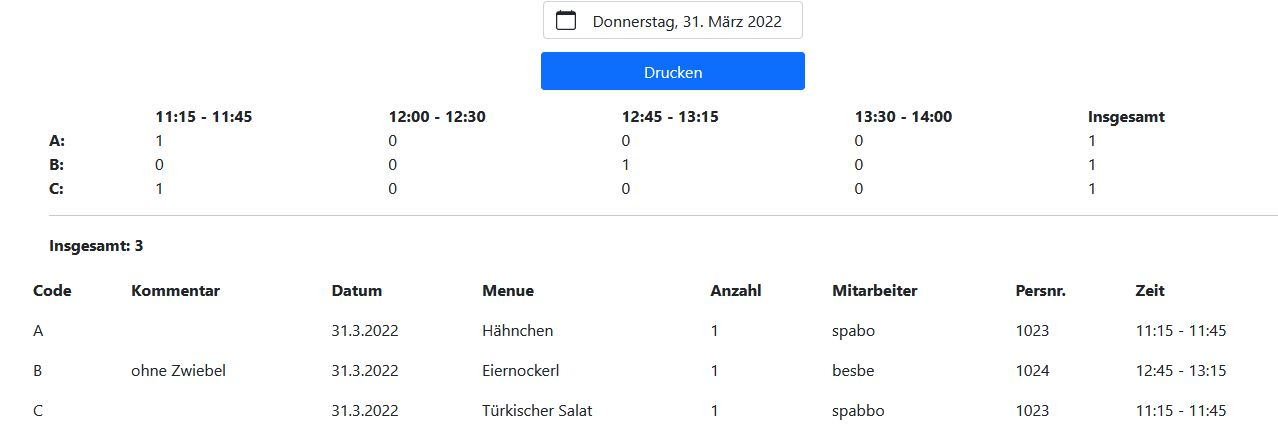
\includegraphics[scale=0.45]{pics/kantine_drucken.JPG}
    \caption{Druckansicht der Kantine}
    \label{fig:impl:CantinePrint}
\end{figure}

\begin{figure}[htp]
    \centering
    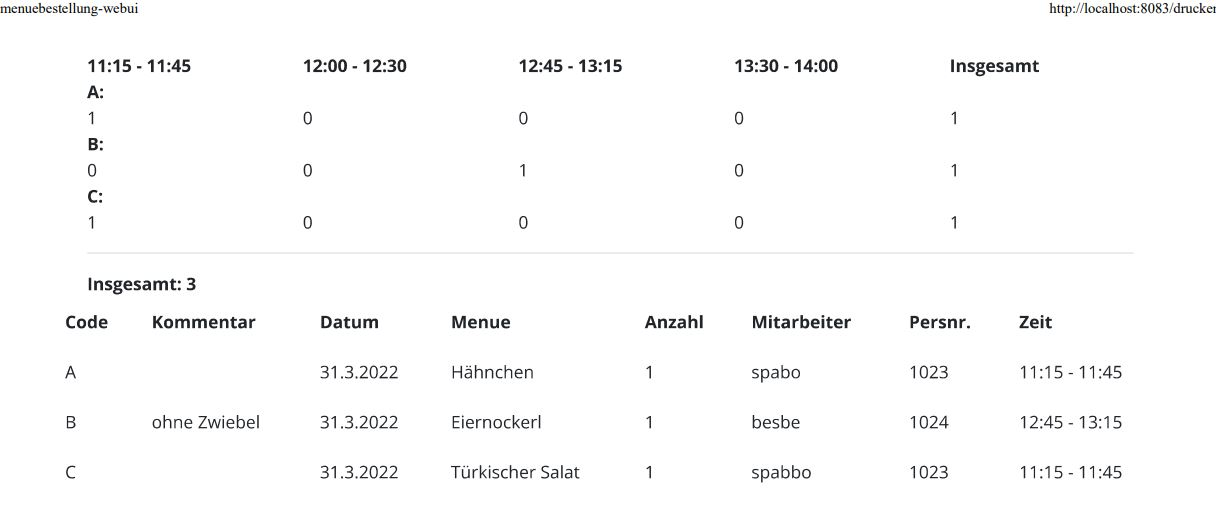
\includegraphics[scale=0.45]{pics/pdf_ansicht.JPG}
    \caption{PDF der Ansicht}
    \label{fig:impl:CantinePrintPDF}
\end{figure}
\pagebreak

\section{Android-App}
Die Android App ist in verschiedene Packages unterteilt: 

\begin{itemize}
    \item api
    \item composable 
    \item dataClasses
\end{itemize}

Im api Package sind gibt es ein ApiObject, welcher alle URL's beinhaltet. Dies erleichtert die Konfiguration der Android Anwendung im Bezug auf das Kommunizieren mit dem Backend.
Noch dazu gibt es die ApiService Klasse, die alle Requests erledigt. 


ApiObject:
\begin{lstlisting}
    object ApiObject {
    @JvmField
    var initMenuesUrl = "http://10.0.2.2:8080/menue/menues/"

    @JvmField
    var bestellungUrl = "http://10.0.2.2:8080/menue/bestellung/"

    @JvmField
    var oeffnungszeiten = "http://10.0.2.2:8080/menue/oeffnungszeiten"

    @JvmField
    var keycloak = "http://10.0.2.2:8082/auth/realms/menuRealm/protocol/openid-connect/token"
}
\end{lstlisting}



Im composable Package sind jene Klassen mit einer View. Diese werden jeweils mit @Composable annotiert. Diese benutzen sich dann
entweder gegenseitig oder die Methoden der ApiService Klasse.
\\*
Im dataClasses Package sind die gebrauchten Entitäten und DTO's (Data Transfer Object).
Hier werden den Menüs, Bestellungen, Öffnungszeiten und dem Acces Token die einzelnen Felder zugewiesen.
\\*

Die MainActivity Klasse ist die Hauptklasse über die die ganze Oberfläche der Android Applikation aufgerufen wird. 
Sie zeigt auch noch die Bottom Navigation Bar, welche zur Navigierung zwischen Übersicht, Bestellansicht und Verlauf verwendet wird.







\pagebreak


\section{Login}
\begin{figure}[htp]
    \centering
    \author{Bozidar Spasenovic}
    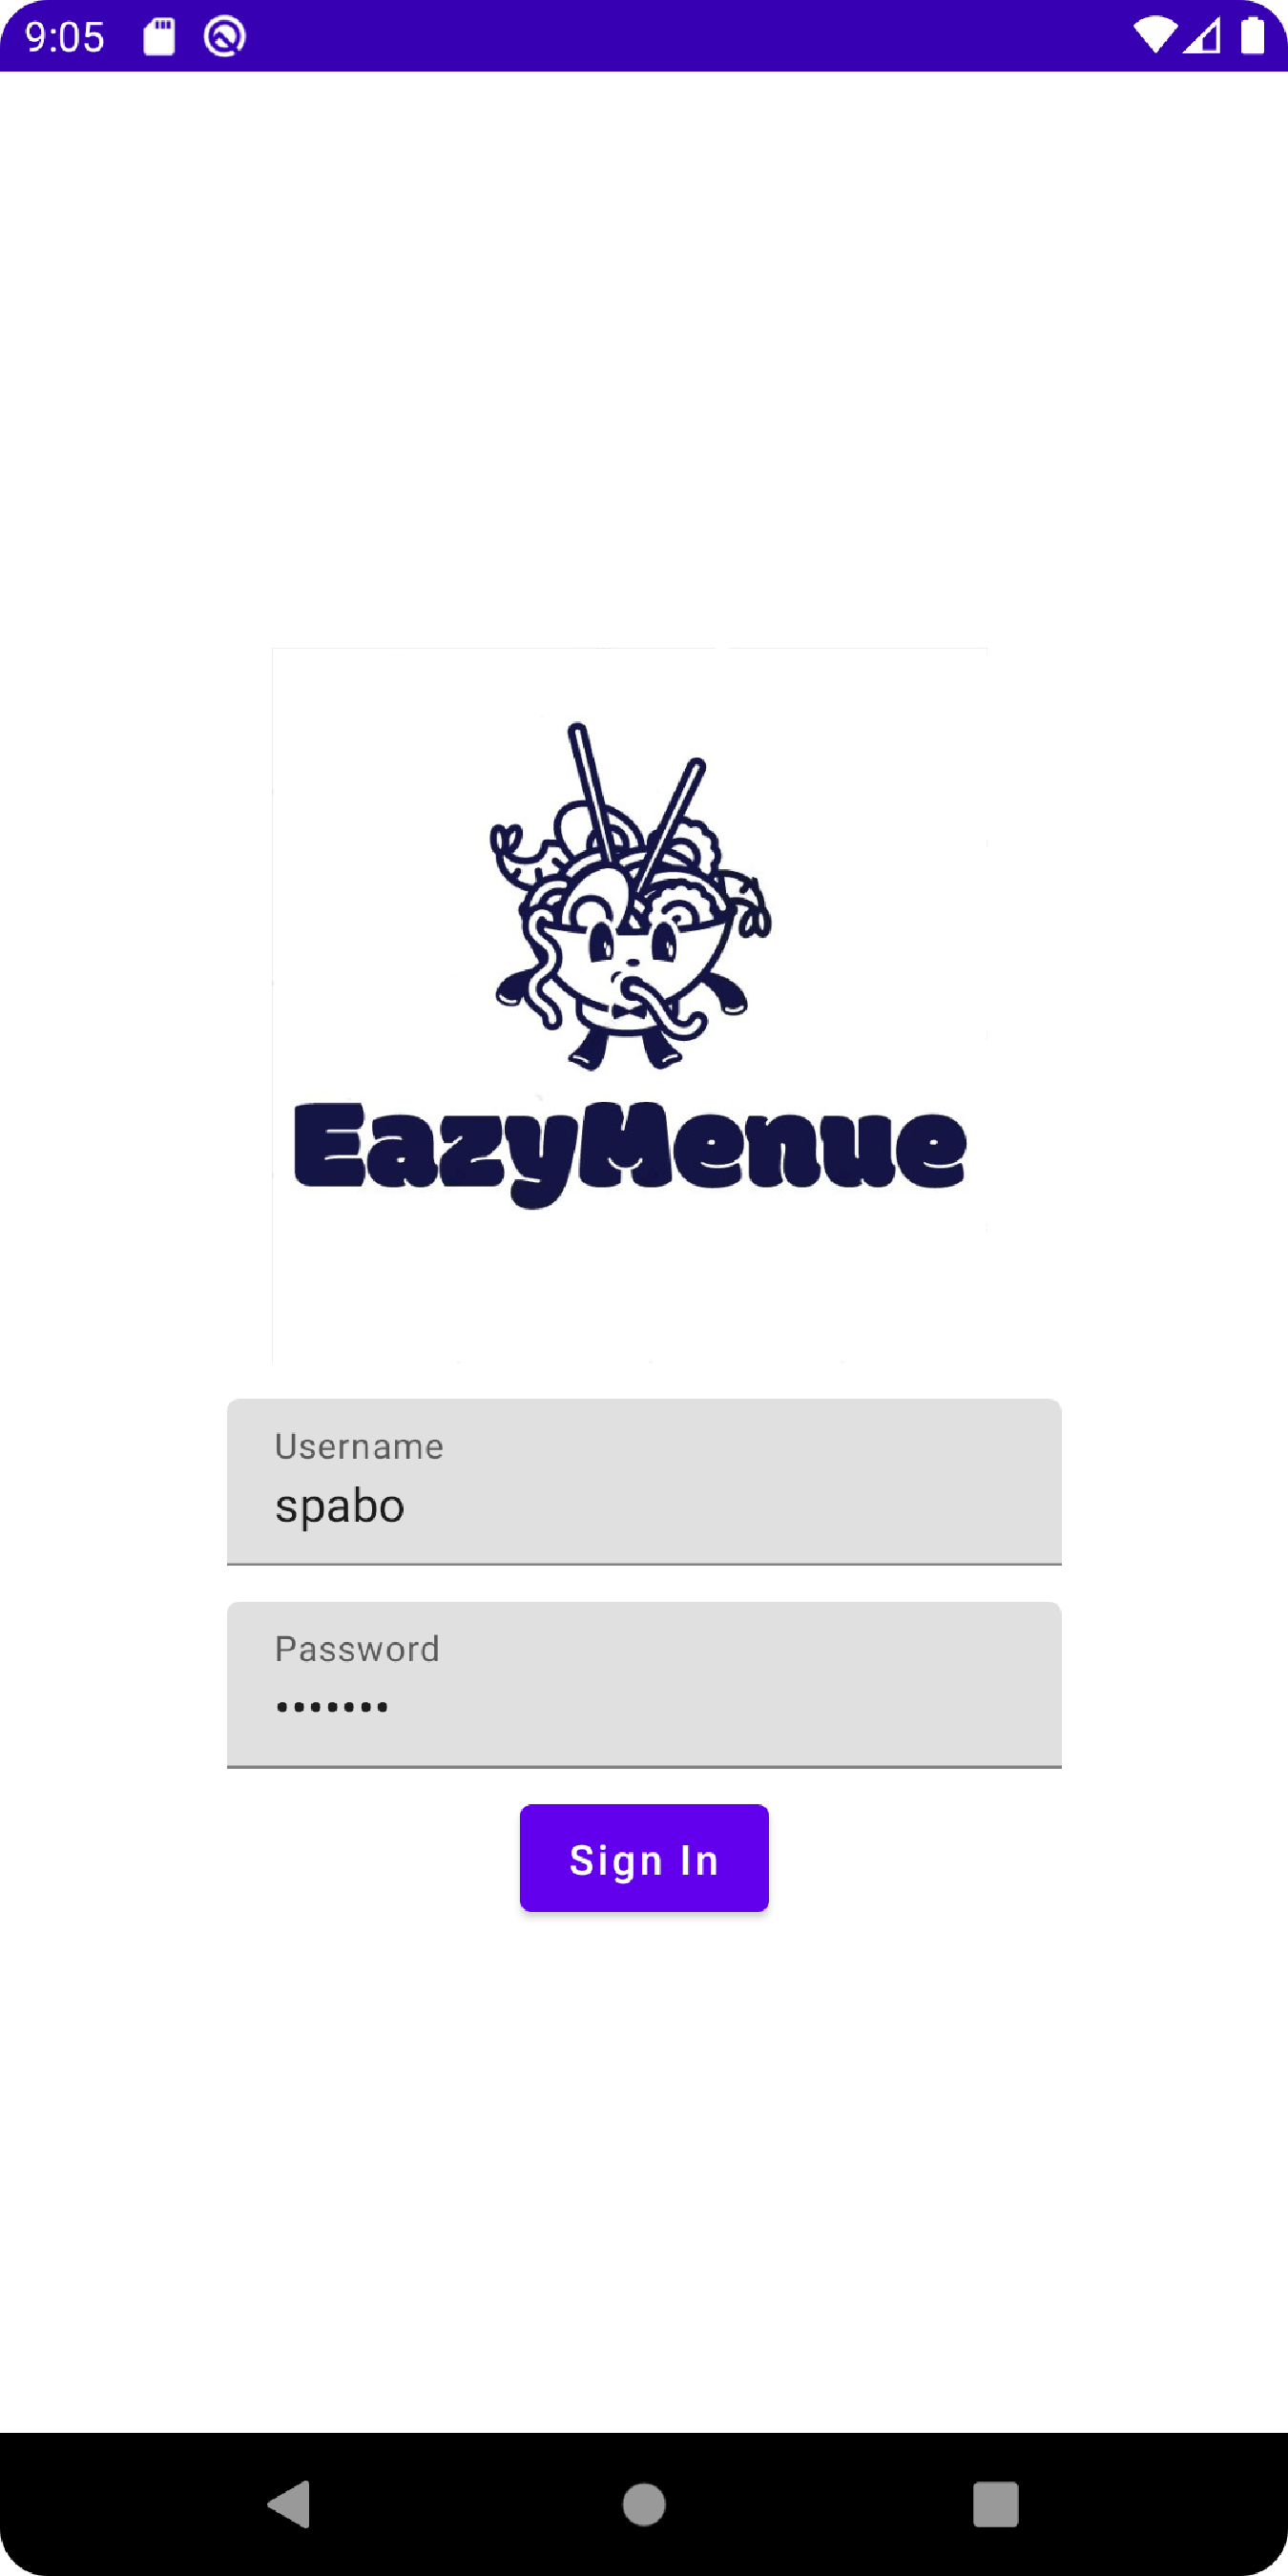
\includegraphics[scale=0.1]{pics/LoginScreenAnndroid.png}
    \caption{Loginscreen Android}
    \label{fig:impl:LoginScreenAnndroid}
\end{figure}

\subsection{Authentification}
Die Authentifizierung erfolgt mit der Methode checkAccessToken, welche nichts anderes macht wie einen Request an den Keycloak zu schicken.
Im Request wird nach einem Access-Token gefragt.
Liefert der Response einen Token, so besteht der User.

\begin{lstlisting}

    Button(onClick = {
        if (!name.isEmpty() && !password.isEmpty() && checkAccessToken()) {

            InitMenues()
            InitBestellungen(name)
            Toast.makeText(
                context,
                "Logged in successfully",
                Toast.LENGTH_SHORT
            ).show()
            isLoggedIn.value = true
            navController.navigate("uebersicht")

        }
    }) {
        Text(text = "Sign In")
    }

\end{lstlisting}




\subsubsection{checkAccessToken()}

Man schickt einen Request an http://10.0.2.2:8082/auth/realms/menuRealm/protocol/openid-connect/token mit einem passendem body.
Im body stehen die Felder die für den Request nötig sind wie zum Beispiel:
\begin{itemize}
    \item die Client ID
    \item der Grant Type 
    \item der Client Secret
    \item der Scope
    \item das Passwort
    \item der Username
\end{itemize}

Als Client wird ein OkHttpClient verwendet. Dieser erstellt einen neuen Aufruf mit dem erstelltem Request. 
Wird im Response ein Token zurückgegeben, so wird er gespeichert. In diesem Schritt werden gleichzeitig mehrere Threads verwendet und deswegen
einen countDownLatch eingebaut. Er ist eine Hilfe für das Warten zwischen einzelnen Threads.
Er wartet also vor der Rückgabe der Methode darauf, dass der Token gespeichert wird. 


\begin{lstlisting}
    client.newCall(request).enqueue(object : Callback {
        override fun onResponse(call: Call, response: Response) {
            response.use {
                if (response.isSuccessful) {
                    accessToken.value = response.body!!.string()
                }
                else{
                    throw IOException("Unexpected code $response")
                }
            }
            countDownLatch.countDown()
        }
        override fun onFailure(call: Call, e: IOException) {
            e.printStackTrace()
            countDownLatch.countDown()

        }
    })
    countDownLatch.await()
    return accessToken.value != ""
\end{lstlisting}


\pagebreak
\section{Übersicht}
\begin{figure}[htp]
    \centering
    \author{Bozidar Spasenovic}
    \includegraphics[scale=0.1]{pics/ÜbersichtViewAndroid.png}
    \caption{Übersicht Android}
    \label{fig:impl:ÜbersichtViewAndroid}
\end{figure}

In der Übersicht kann man mit einem Datepicker ein Datum auswählen, was dazu führt das die jeweiligen Menüs an dem Tag 
als Cards angezeigt werden. Noch dazu wird die jeweilige Vorspeise und Nachspeise angezeigt.

\subsection{Datepicker}
Der Datepicker in Kotlin wird als DatePickerDialog verwendet. Im Dialog wird das ausgewählte Datum in eine temporäre Variable gespeichert
und der Methode getMenuesForDate(date: String) übergeben. Anschließend wird der Wert in der Übersicht angezeigt und man wird wieder zurücknavigiert.

\begin{lstlisting}
    val datePickerDialog = DatePickerDialog(
        context,
        { _: DatePicker, year: Int, month: Int, dayOfMonth: Int ->
            var temp = month.inc()
            if (dayOfMonth >= 1 && dayOfMonth <= 9) {

                if (temp.toString().length == 1) {
                    date.value = "$year-0${temp}-0$dayOfMonth"
                } else {
                    date.value = "$year-${temp}-0$dayOfMonth"
                }
            } else {
                if (temp.toString().length == 1) {
                    date.value = "$year-0${temp}-$dayOfMonth"
                } else {
                    date.value = "$year-${temp}-$dayOfMonth"
                }
            }
            getMenuesForDate(date.value)
            uebersichtDate.value = date.value
            navController.navigate("uebersicht")
        }, year, month, day
    )
\end{lstlisting}


\subsubsection{getMenuesForDate}
Die Methode beinhaltet den Filteralgorhytmus von Menüs für einen Tag. Es wird erstmals überprüft ob das jetzige Datum voor dem Datum des Menüs ist
und ob die jetzige Zeit, falls man am selben Tag bestellt, vor neun Uhr ist. Sind die beiden Bedingungen erfüllt so wird es dem Mitarbeiter ermöglicht ein Menü auszuwählen.

\begin{lstlisting}
    if (date <= LocalDateTime.now().toString().take(10) && LocalDateTime.now().hour >= 9) {
        menueIsInThePast.value = true
    } else {
        menueIsInThePast.value = false
    }
    menuesFilteredByDate = menuesFilteredByDate - menuesFilteredByDate
    menues.sortedBy { menue -> menue.date }.sortedBy { menue -> menue.code }.forEach { menu ->
        if (menu.date == date) {
            menuesFilteredByDate = menuesFilteredByDate.plusElement(menu)
        }
    }
\end{lstlisting}

Dazu wird die Methode getOeffnungszeiten() aufgerufen die die notwendigen Zeiten mit freien Sitzplätzen aus dem Backend holt und anzeigt.


\begin{lstlisting}
    client.newCall(request).enqueue(object : Callback {
        override fun onFailure(call: Call, e: IOException) {
            e.printStackTrace()
        }

        override fun onResponse(call: Call, response: Response) {
            response.use {
                if (!response.isSuccessful) throw IOException("Unexpected code $response")

                val gson = GsonBuilder().create()

                val collectionType: Type =
                    object : TypeToken<Collection<Oeffnungszeiten?>?>() {}.type
                oeffnungszeiten = gson.fromJson(response.body!!.string(), collectionType)
            }
        }
    })
\end{lstlisting}

\subsection{Card}
\cite{Card}
\author{Bozidar Spasenovic}

Eine Card wird verwendet um mehrere Items schön beisammen zu halten. Man kann die Card konfigurieren indem man die Erhöhung und den Schatten erhöht.
Außerdem kann man Formen definieren wie zum Beispiel:

\begin{itemize}
    \item Rectangle Shape
    \item Circle Shape
    \item Rounded Corner Shape
    \item Cut Corner Shape
\end{itemize}

Wie bei fast allen anderen Items, ist es auch hier möglich die Darstellung zu ändern.

\begin{itemize}
   \item modifier
   \item shape
   \item backgroundColor
   \item contentColor
   \item border
   \item elevation
   \item content
\end{itemize}

Dargestellt wird es mit einer einfachen Funktion.


\begin{lstlisting}
    Card {
        Text(
            text = "Card"
        )
    }
\end{lstlisting}

Um die einzelnen Modifizierungen einzubauen, gibt man der Funktion die jeweiligen Parameter mit.

\begin{lstlisting}
    Card(
        modifier: Modifier = Modifier,
        shape: Shape = RectangleShape(5.dp),
        backgroundColor: Color = Color.Transparent,
        contentColor: Color = Color.Red,
        elevation: Dp = 10.dp
    ) {
        Text(
            text = "Card"
        )
    }
\end{lstlisting}





\subsection{Log out}
Der Mitarbeiter hat eine Möglichkeit sich auch aus der App auszuloggen. Das erfolgt durch den Sign out Button.
\begin{figure}[htp]
    \centering
    \author{Bozidar Spasenovic}
    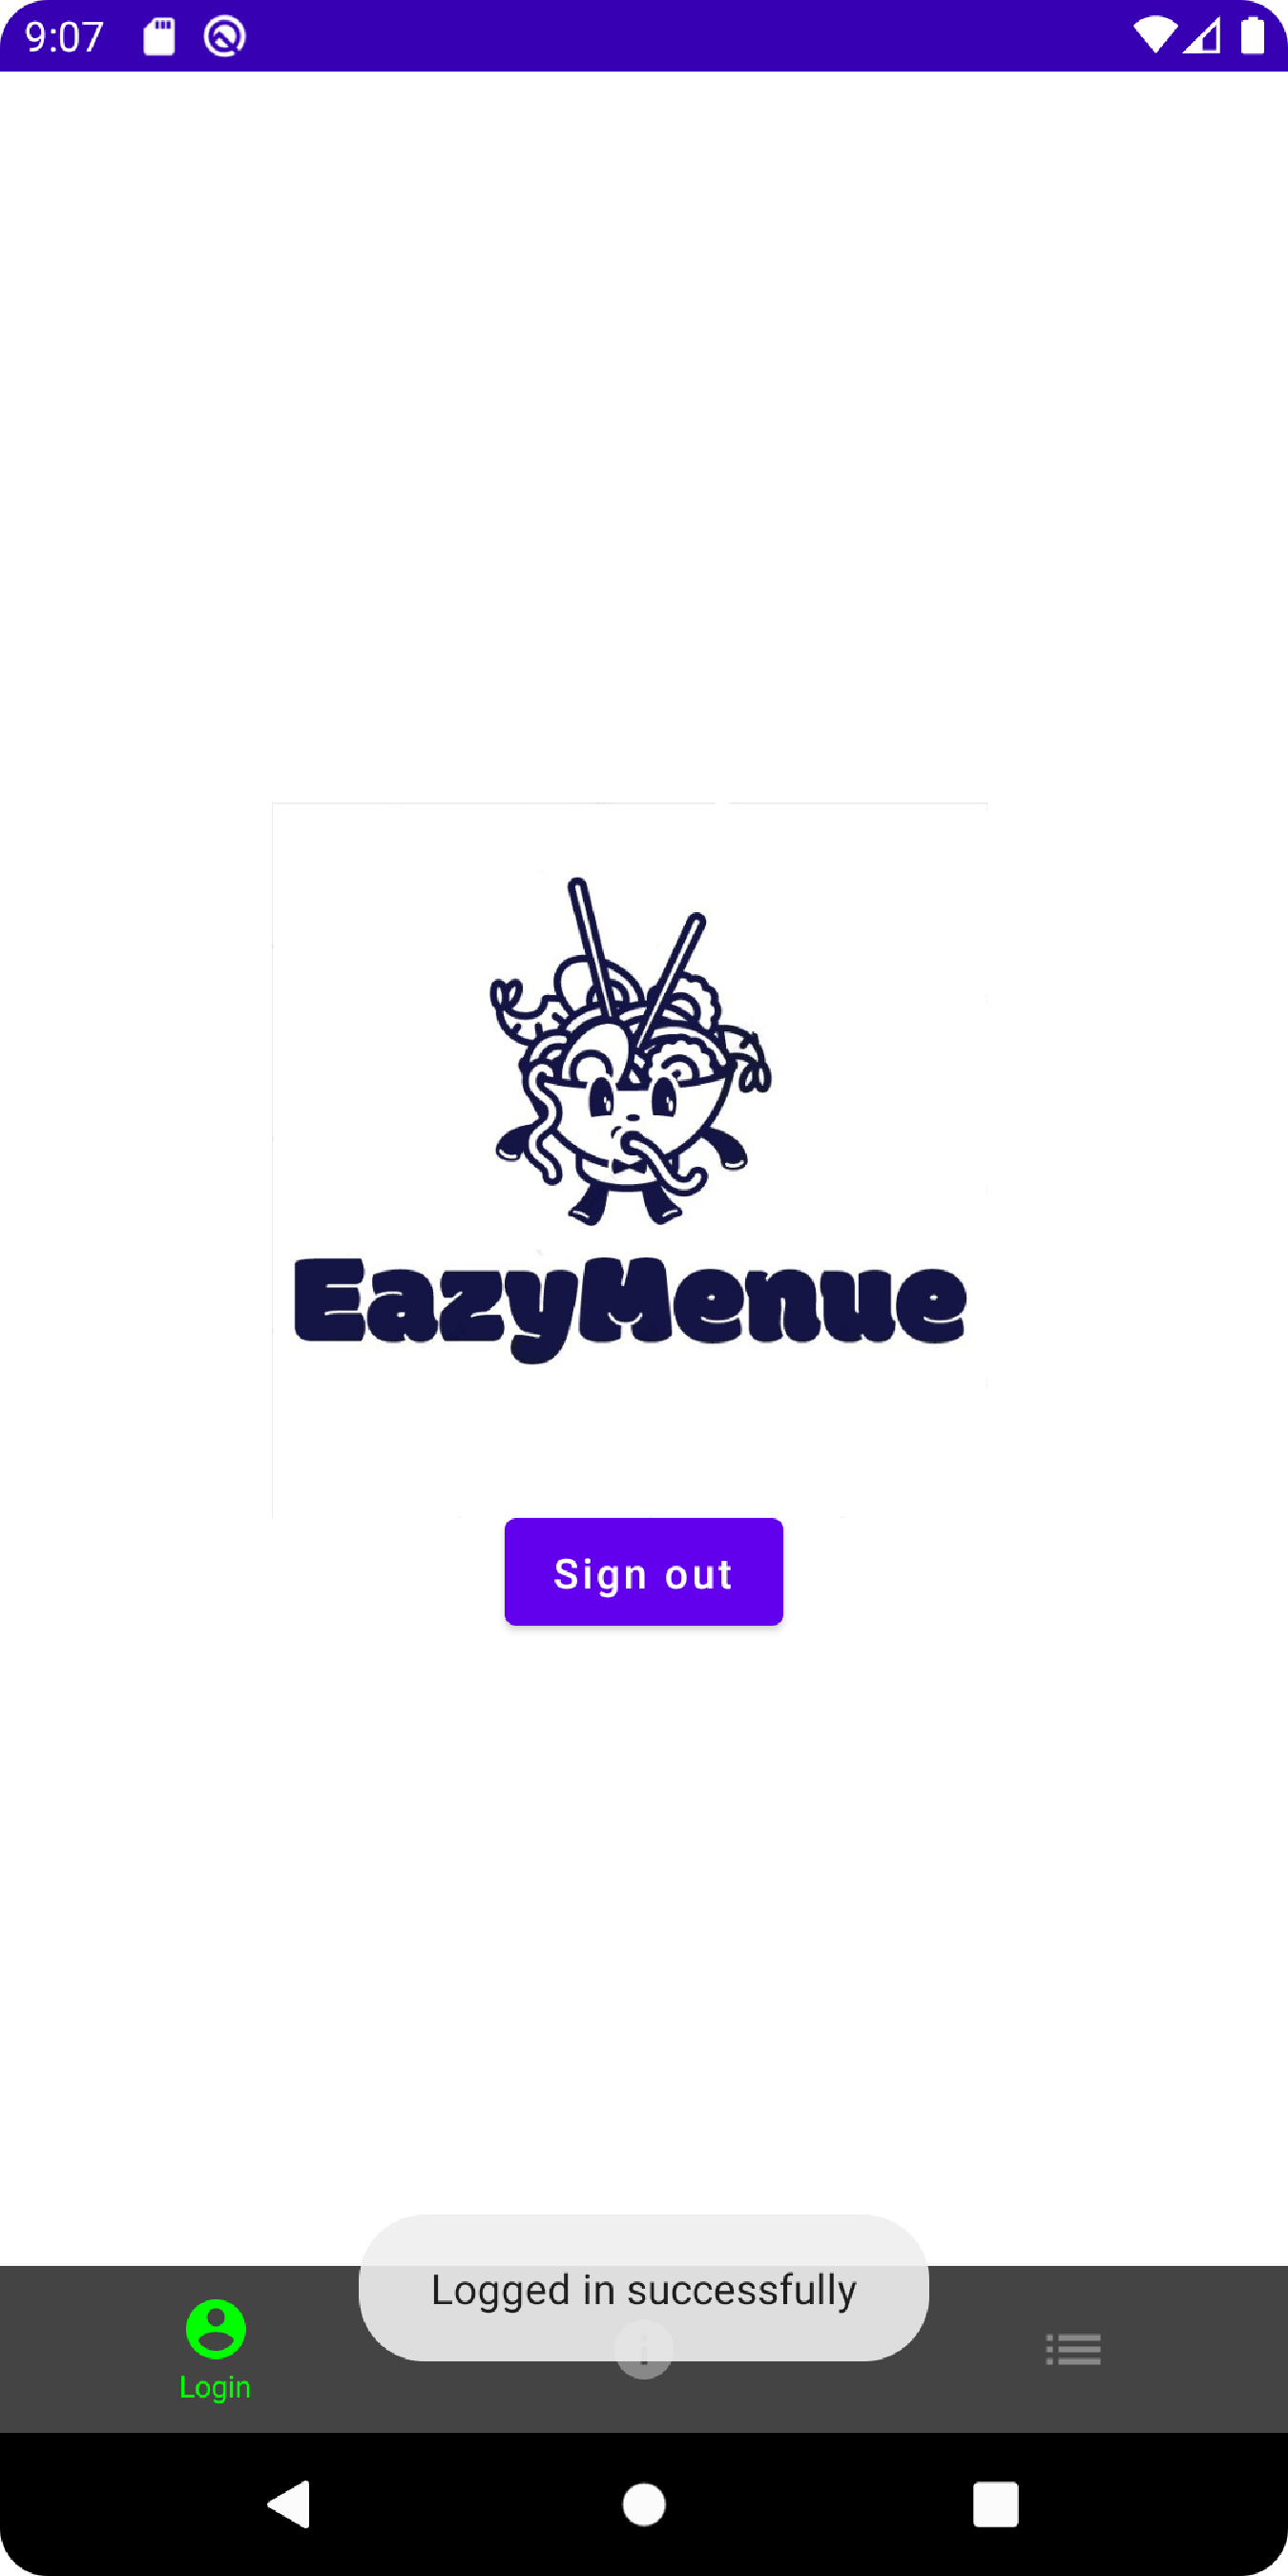
\includegraphics[scale=0.09]{pics/SignOutScreenAnndroid.png}
    \caption{Signout Android}
    \label{fig:impl:SignOutScreenAndroid}
\end{figure}

Nach dem Einloggen wird die Methode InitBestellungen() aufgerufen. Ihre Aufgabe ist es den derzeitigen Bestellungsverlauf des Mitarbeiters zu initialisieren.
Den kann man dann auch in der Verlaufsansicht sehen. Noch dazu wird die Methode InitMenues() aufgerufen und somit alle erstellten Menüs geholt.


\begin{lstlisting}
    client.newCall(request).enqueue(object : Callback {
        override fun onFailure(call: Call, e: IOException) {
            e.printStackTrace()
        }

        override fun onResponse(call: Call, response: Response) {
            response.use {
                if (!response.isSuccessful) throw IOException("Unexpected code $response")

                val gson = GsonBuilder().create()

                val collectionType: Type =
                    object : TypeToken<Collection<Menue?>?>() {}.type


                menues = gson.fromJson(response.body!!.string(), collectionType)
            }
        }
    })
\end{lstlisting}


Der Response wird so benutzt, dass man als erstes mit dem GsonBuilder ein Gson-Objekt erstellt
 was das Umwandeln von JSON-Objekten zu Kotlin Objekten ermöglicht. 
Dieses Objekt wird verwendet um ein JSON-Objekt in ein Kotlin-Objekt umzuwandeln. 
Damit man Gson verwendetn kann, benötigt man die Abhängigkeit com.google.code.gson:gson:2.8.9.
Mit dem collectionType wird definiert in was für ein Typ das JSON-Objekt umgewandelt werden soll.
Abschliesend wird vom Responsebody eine Collection von allen mitgegebenen Bestellungen erstellt und gespeichert.


\pagebreak

\section{Verlauf}

Der Verlauf ist eine einfache Liste (LazyColumn) von den ganzen Bestellungen des Users.
Es wird der Menüname, das Bestelldatum und das Datum des Menüs angezeigt.
Ist die Bestellung stornierbar, so wird eine Mülltonne als Icon angezeigt. 
Durch das Draufklicken auf die Mülltonne, wird die Bestellung storniert.

\begin{figure}[htp]
    \centering
    \author{Bozidar Spasenovic}
    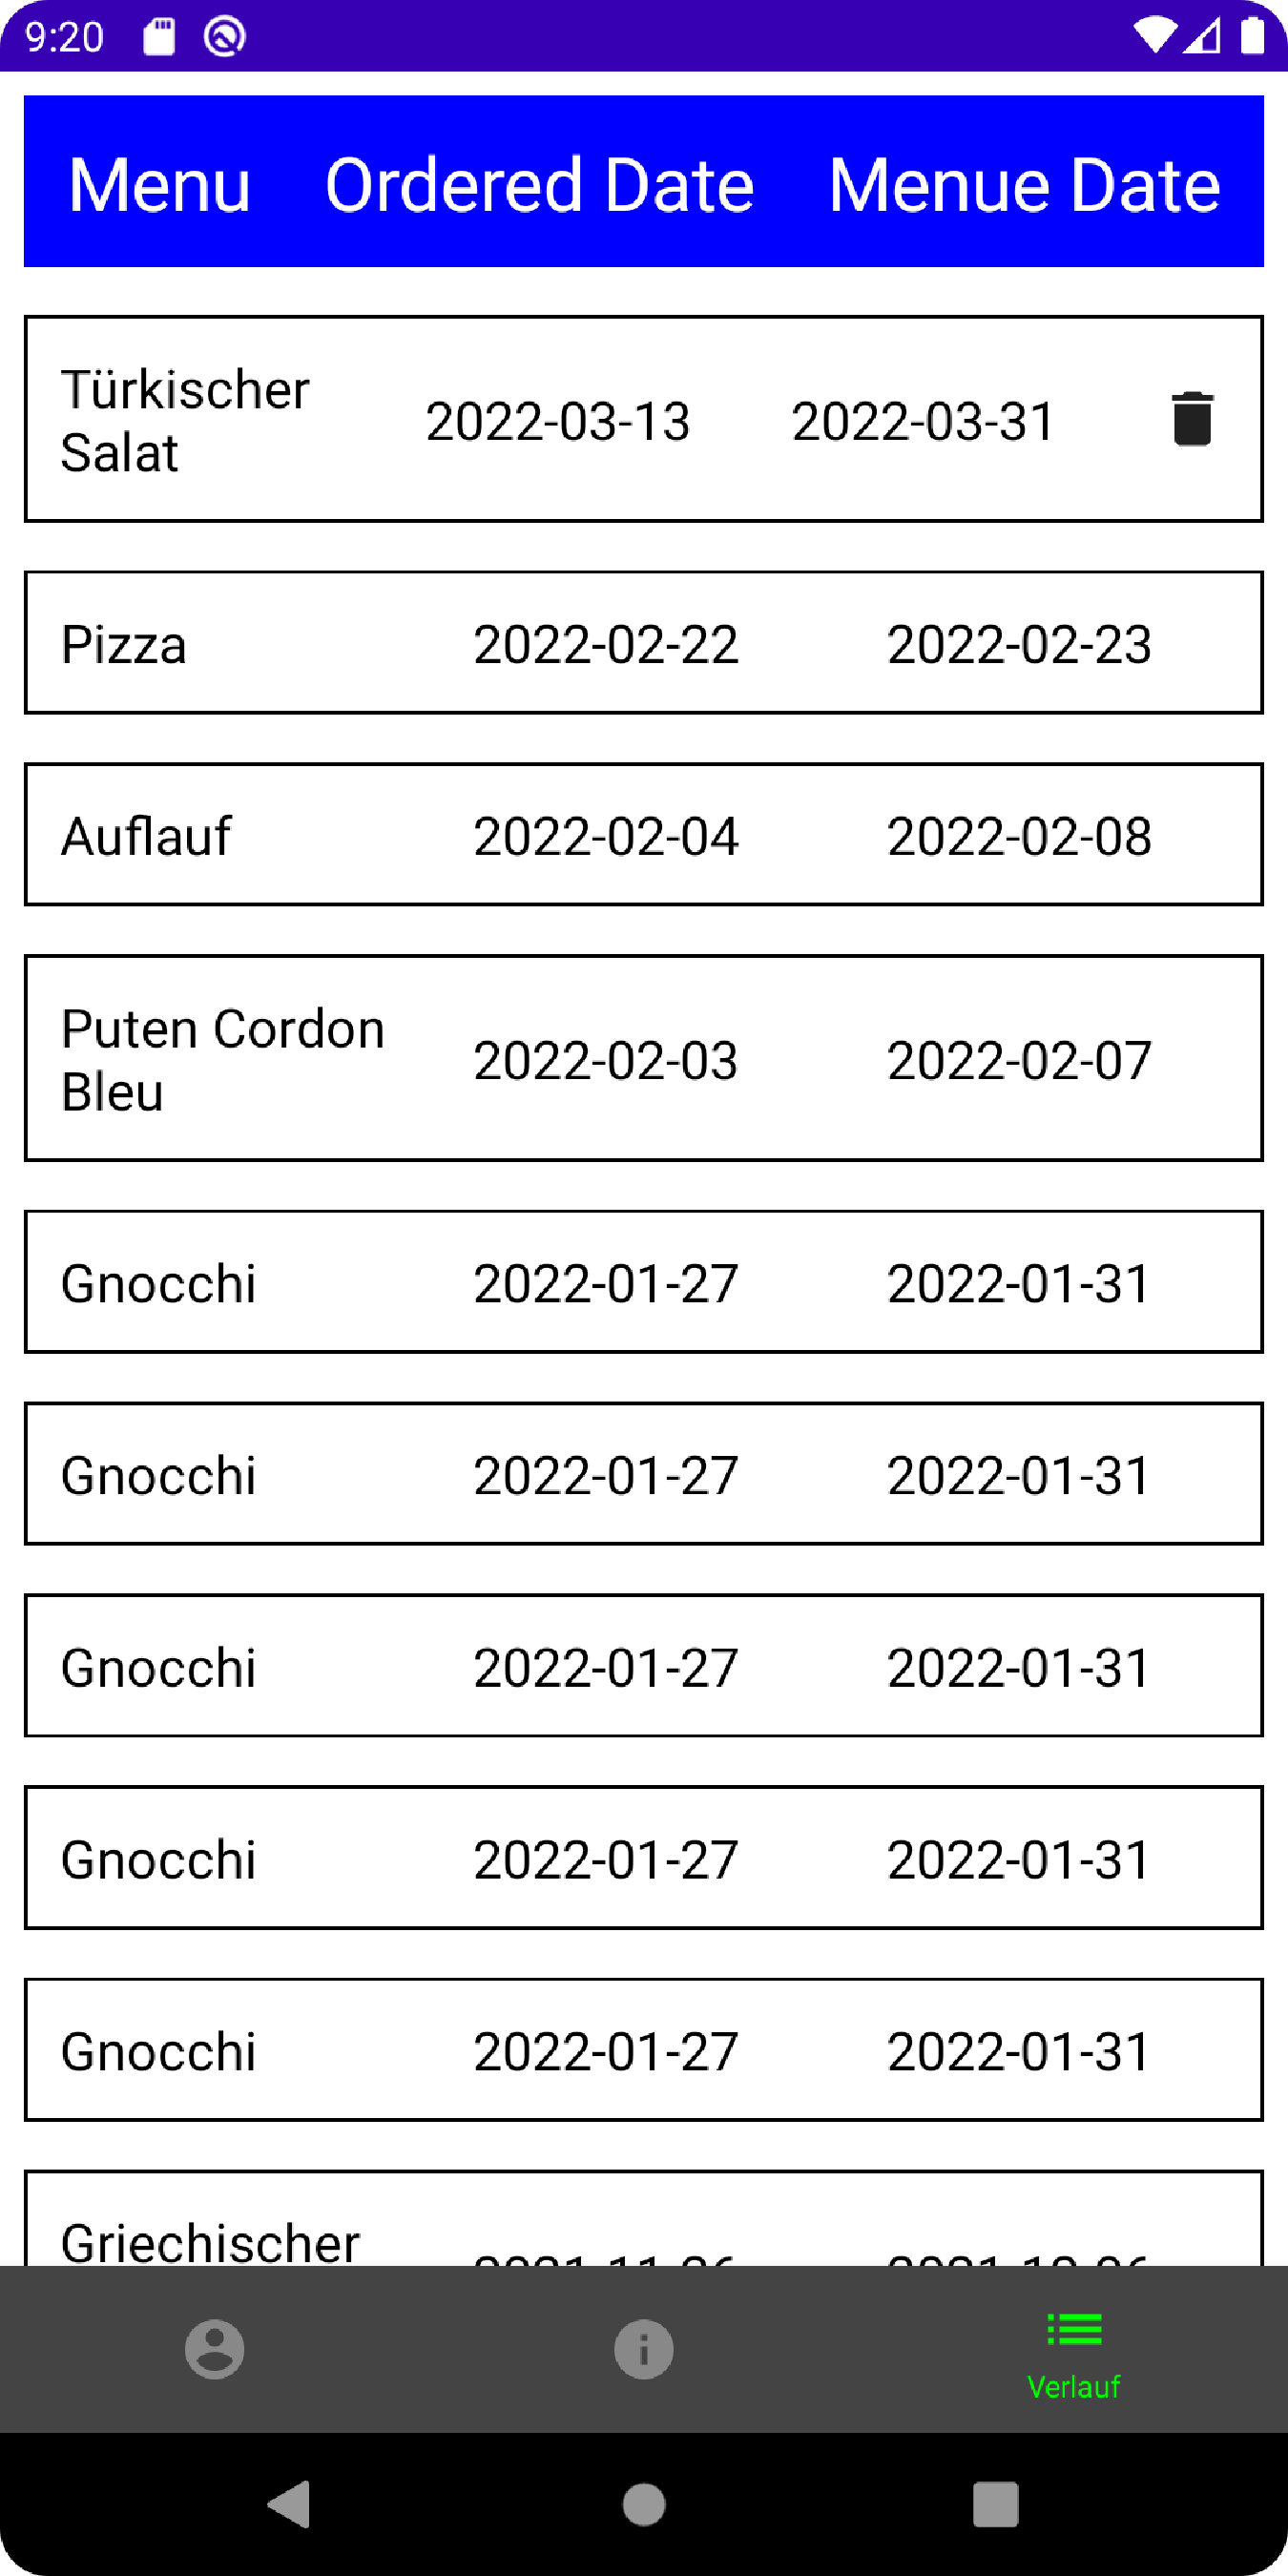
\includegraphics[scale=0.09]{pics/VerlaufAndroid.png}
    \caption{VerlaufAndroid Android}
    \label{fig:impl:VerlaufAndroid}
\end{figure}


Es wird ein PUT auf die URL http://10.0.2.2:8080/menue/bestellung?id=\$menuId was im backend das Löschen zur jeweiligen Menü Id ausübt.
Falls ein erfolgreicher Response zurückkommt, so wird die InitBestellungen()-Methode zum neu Laden des Verlaufes aufgerufen.

\begin{lstlisting}
    client.newCall(request).enqueue(object : Callback {
        override fun onFailure(call: Call, e: IOException) {
            e.printStackTrace()
        }

        override fun onResponse(call: Call, response: Response) {
            response.use {
                if (!response.isSuccessful){
                    throw IOException("Unexpected code $response")
                }

                InitBestellungen(currUser.value)
            }
        }
    })
\end{lstlisting}


\pagebreak


\section{Bestellansicht}

In der Bestellansicht werden die Felder Menü, Von und das Datum automatisch in ein Readonly Text Field gespeichert.
Man kann dann die Anzahl angeben, für wen man es bestellen möchte und auch zwischen vier Zeiten aussuchen. 

\begin{figure}[htp]
    \centering
    \author{Bozidar Spasenovic}
    \includegraphics[scale=0.09]{pics/BestellübersichtAndroid.png}
    \caption{Bestellansicht Android}
    \label{fig:impl:BestellübersichtAndroid}
\end{figure}

\subsection{postBestellung()}
Nach dem Abschließen wird die postBestellung()-Methode aufgerufen. Sie erstellt einen Requestbody mit den eingegebenen Werten
und schickt es mittels POST an die "http://10.0.2.2:8080/menue/bestellung/" URL. Dieser Endpoint führt dann die Anfrage durch und schickt einen Response zurück.
Wichtig dabei ist es den richtigen Media-Type zu definieren. 

Die Anfrage und Antwort:
\begin{lstlisting}
    client.newCall(requestDto).enqueue(object : Callback {
        override fun onFailure(call: Call, e: IOException) {
            e.printStackTrace()
        }

        override fun onResponse(call: Call, response: Response) {
            response.use {
                if (!response.isSuccessful) throw IOException("Unexpected code $response")

                response.headers.get("orderedBy")?.let { it1 -> InitBestellungen(it1) }
            }
        }
    })
\end{lstlisting}


\subsubsection{Interface Callback}
\cite{Callback}
Da Java keine \textit{Pointer} Konzepte verwendet, gibt es die Callbackfunktion nicht wie in C oder C++.
Da hingegen gibt es das sogenannte Callback Interface.
Jede Schnittstelle hat einen Speicherort. Diese wird dann, anstatt der Funktion selbst, übergeben und verwendet.
\\*

\subsubsection{onResponse}








\begin{spacing}{1}
\chapter{Zusammenfassung}
\end{spacing}
\section{Zusammenfassung}
\author{Bozidar Spasenovic}
Die vorliegende Diplomarbeit beschäftigt sich mit einer Kantinenwebapp und einem zusätzlichen Android Client, die zur Essensbestellung
verwendet werden. Ziel dieser Diplomarbeit ist es allen Mitarbeitern der Oberösterreichischen Versicherung ein Benutzerfreundliches Bestellsystem
bereitzustellen und somit auf keine veraltete Technologie beschränkt zu sein. 

Das Ergebnis ist eine benutzerfreundliche Webapp mit zwei Arten von Usern. Die User bekommen durch ihr Bestellverlauf vorgeschlagene
Menüs angezeigt. Der User kann dadurch auch gleichzeitig sehen, welche Arten von Gerichten er bevorzugt.

\section{Ausblick}
Die weiteren Schritte für das Projekt ist die Freigabe für mehrere Firmen mit einer Kantine. Um das zu schaffen benötigt man einen Server
über den man einen Docker-Container mit dem Backend laufen lässt um dannach die Webapp im Browser aufrufen zu können. Noch ein
weiterer Schritt wär es die Webapp auf mehrere Sprachen zu erweitern um auch auf Internationalerebene eine Verwendung zu finden.

\newpage
\pagenumbering{Roman}
\setcounter{page}{\value{RPages}}
\newacronym{guid}{GUID}{Globally Unique Identifier}
\newacronym{jit}{JIT}{Just In Time Compiler}
\newacronym{nfc}{NFC}{Near Field Communication}
\newacronym{rfid}{RFID}{Radio Frequency Identification}

% Usage:
% \gls{label} lowercase in text
% \Gls{label} Uppercase in text
% \newacronym{label}{abbrev}{full}
% \newglossaryentry{label}{settings}



%\setlength{\glsdescwidth}{0.8\linewidth}
\glsnogroupskiptrue
\printglossary[title=Glossar,toctitle=Glossar] %,style=long]
\spacing{1}{
%\bibliographystyle{IEEEtran}
\bibliographystyle{ieeetrande}
\bibliography{bib}
}
\listoffigures
\listoftables
%\listoflistings
\appendix
\addchap{Anhang}
\section{Protokolle}
\begin{table}
    
    \begin{tabular}{|p{3cm}|p{10cm}|  }
        \hline
        Datum & 25-10-2021\\
        \hline
        Anwesende & Benjamin Besic, Bozidar Spasenovic, David Ignjatovic\\
        \hline
        Zwischenstand&  Das Programm ist lauffähig und erfüllt alle usecases. \\
        \hline
        Bis zum nächsten mal &  Schriftliche Diplomarbeit\\
        \hline
        
    \end{tabular}
    \caption{Protokoll 25-10-2021}
    \label{tab:my_label}
\end{table}
\begin{table}
    \begin{tabular}{ |p{3cm}|p{10cm}|   }
        \hline
        Datum & 12-11-2021\\
        \hline
        Anwesende & Benjamin Besic, Bozidar Spasenovic, David Ignjatovic\\
        \hline
        Zwischenstand& Diagramme wurden gezeigt mit dummy werten.\\
        \hline
        Bis zum nächsten mal &  Food Recommender, Android, Schriftlicher Teil \\
        \hline
    \end{tabular}
    \caption{Protokoll 12-11-2021}
    \label{tab:my_label}
\end{table}
\begin{table}
    \begin{tabular}{ |p{3cm}|p{10cm}|  }
        \hline
        Datum & 26-11-2021\\
        \hline
        Anwesende & Benjamin Besic, Bozidar Spasenovic, David Ignjatovic\\

        \hline
        Zwischenstand&  erste Version Android, Recommender, schriftlicher Teil
    
    \\
        \hline
        Bis zum nächsten mal &  

       Android: restlichen Fragmente,logik
        

    frontend mit backend verbinden

    grafiken mit neuem backend

    statistiken

    versuchen den schriftlichen Teil für einen ersten Überblick fertigstellen


    
    \\
        \hline
    \end{tabular}
    \caption{Protokoll 26-11-2021}
    \label{tab:my_label}
\end{table}
\begin{table}
    \begin{tabular}{ |p{3cm}|p{10cm}|  }
        \hline
        Datum & 10-12-2021\\
        \hline
        Anwesende & Benjamin Besic, Bozidar Spasenovic, David Ignjatovic\\

        \hline
        Zwischenstand&  Jetpack compose

        Es wurde das neue Projekt gezeigt, welches von XML auf Jetpack compose umgeschrieben.
        Die App ist zurzeit mit statischen werten befüllt.
        Problem ist das Jetpack compose relativ neu ist, und wenig informationsquellen online zur verfügung stehen.
        1.2. Backend
        
        Backend ist im groben und ganzen fertig. Logic für die Statistiken wird noch erledigt.
        1.3. Recommender
        
        Frontend wurde fertiggestellt für den Recommender.
        \\
        \hline
        Bis zum nächsten mal &  



        Statistik (Backend/Frontend) wird fertiggestellt

        Android App wird erweitert
    
    
    
    \\
        \hline
    \end{tabular}
    \caption{Protokoll 10-12-2021}
    \label{tab:my_label}
\end{table}
\begin{table}
    \begin{tabular}{ |p{3cm}|p{10cm}|   }
        \hline
        Datum & 06-01-2022\\
        \hline
        Anwesende & Benjamin Besic, Bozidar Spasenovic, David Ignjatovic\\

        \hline
        Zwischenstand& Es wurde das neue Projekt gezeigt, welches von XML auf Jetpack compose umgeschrieben.
        Die App ist zurzeit mit statischen werten befüllt.
        Problem ist das Jetpack compose relativ neu ist, und wenig informationsquellen online zur verfügung stehen.
        
        Backend ist im groben und ganzen fertig. Logic für die Statistiken wird noch erledigt.
        
        Frontend wurde fertiggestellt für den Recommender.\\
        \hline
        Bis zum nächsten mal &  





        Android app muss noch fertig gemacht werden. (Spasenovic)

        KeyCloak mit JetPackCompose
    
        Statistiken anzeigen
    
        Recommender und Statistiken evt. erweitern (Ignjatovic und Besic)
    
    


    
    \\
        \hline
    \end{tabular}
    \caption{Protokoll 06-01-2022}
    \label{tab:my_label}
\end{table}
\begin{table}
    \begin{tabular}{ |p{3cm}|p{10cm}|  }
        \hline
        Datum & 28-01-2022\\
        \hline
        Anwesende & Benjamin Besic, Bozidar Spasenovic, David Ignjatovic\\

        \hline
        Zwischenstand& 

        KeyCloak funktioniert jetzt
    
        Bestellungen werden angezeigt
    
   Probleme
    
        Beim Bestellen kommt ein fehler (unsupported mediatype).
    
        Login button muss 2 mal gedrückt werden.
    
            möglicher Fehler: api läuft asynchron
    
        hartkodierte urls vermeiden
    
    \\
        \hline
        Bis zum nächsten mal &  

        Schriftlich weiterschreiben / Beisc, Ignjatovic (evt. Spasenovic)
    
            verwendete Technologien
    
            implementierung
    
        Android Projekt verschönern (Spasenovic)
    
        Automatisierte Test
    \\
        \hline
    \end{tabular}
    \caption{Protokoll  28-01-2022}
    \label{tab:my_label}
\end{table}
\begin{table}
    \begin{tabular}{ |p{3cm}|p{10cm}|  }
        \hline
        Datum & 04-02-2022\\
        \hline
        Anwesende & Benjamin Besic, Bozidar Spasenovic, David Ignjatovic\\

        \hline
        Zwischenstand& 

        Was funktioniert:

    Login noch nicht ganz fertig - KeyCloak fehlt

    Logik hinter der App funktioniert

    Was geht leider noch nicht

    Post funktioniert nicht ganz

    Statistiken in der Android App gehen nicht




    
    \\
        \hline
        Bis zum nächsten mal & 





        Kotlin Login verbessern / Spasenovic

        Backend Bug fixen / Ignjatovic
    
        schriftlicher Teil (Implementierung) / evt (alle)
    
    


    
    
    
    \\
        \hline
    \end{tabular}
    \caption{Protokoll 04-02-2022}
    \label{tab:my_label}
\end{table}
\begin{table}
    \begin{tabular}{ |p{3cm}|p{10cm}|  }
        \hline
        Datum & 23-02-2022\\
        \hline
        Anwesende & Benjamin Besic, Bozidar Spasenovic, David Ignjatovic\\

        \hline
        Zwischenstand& Was geht nicht

        Probleme mit dem formbody in postBestellung
    
            403 MediaType not supported
    
    Was fehlt noch
    
        Bestellung
    
        eventuelle verschönerungen
    
     Was wurde gemacht
    
        Login gefixt mit CountDownLatch()
    
        Verlauf
    
    \\
        \hline
        Bis zum nächsten mal &  

        Schriftlicher Teil / alle
    
            Implementierung / Verwendete Technologien
    
        Bestellung fixen / Spasenovic
    
            Android
    
        Unit Test / Ignjatovic
    
            Backend
    
    \\
        \hline
    \end{tabular}
    \caption{Protokoll 23-02-2022}
    \label{tab:my_label}
\end{table}




\begin{table}
    \begin{tabular}{ |p{3cm}|p{10cm}|   }
        \hline
        Datum & 17-03-2022\\
        \hline
        Anwesende & Benjamin Besic, Bozidar Spasenovic, David Ignjatovic\\

        \hline
        Zwischenstand& 



        bestellung funktioniert jetzt

        fehler war falscher name des Atributes

        personalnummer und orderFor war null



    \\
        \hline
        Bis zum nächsten mal &  Android

        bessere package namen verwenden
    
        Ip Addressen nicht hardcoden
    
     Schriftlich
     Planung
    
        liegt verloren
    
        sagt wenig aus
    
        Datenmodel Diagramme
    
        Datenmodel Diagramme zur Implementierung verschieben.
    
        Eventuell Planung zur Implementierung.
    
        Mockups erweitern mit Text.
    
        UseCases zur Implementierung
    
     Backend
    
        Swagger wäre nicht schlecht und dann im schriftlichen Teil einbauen
    
        Im schriftlichen Teil
    
            Weniger Code bei attribute
    
    \\
        \hline
    \end{tabular}
    \caption{Protokoll 17-03-2022}
    \label{tab:my_label}
\end{table}
\begin{table}
    \begin{tabular}{ |p{3cm}|p{10cm}|   }
        \hline
        Datum & 25-03-2022\\
        \hline
        Anwesende & Benjamin Besic, Bozidar Spasenovic, David Ignjatovic\\

        \hline
        Zwischenstand& 

        Request in eigen File geschrieben
    
        Component im schriftlichen Teil beschrieben
    
    \\
        \hline
        Bis zum nächsten mal & 

        abstract
    
        zusammenfassung
    
        hinten ausführliche zusammenfassung könnte mehrere Seiten haben
    
     \\
        \hline
    \end{tabular}
    \caption{Protokoll 25-03-2022}
    \label{tab:my_label}
\end{table}
\begin{table}
    \begin{tabular}{ |p{3cm}|p{10cm}|   }
        \hline
        Datum & 01-04-2022\\
        \hline
        Anwesende & Benjamin Besic, Bozidar Spasenovic, David Ignjatovic\\

        \hline
        Zwischenstand& 

        Github Actions/Packages geschrieben
    
        Implementierung geschrieben
    
    \\
        \hline
        Bis zum nächsten mal &  
    
    \\
        \hline
    \end{tabular}
    \caption{Protokoll 01-04-2022}
    \label{tab:my_label}
\end{table}
\end{document}

